\chapter{Design Patterns for Pattern Layering}\label{cha:patterns}

This chapter contains a catalog of design patterns related to material layering. The pattern catalog presents the core of this work and incorporates all previous results and analysis. It combines the results of the previous research and presents them in practical patterns. The patterns are categorized and structured in a hierarchical way. This is supposed to simplify the process of finding design patterns related to the actual problem. The patterns start from high level decisions of how and if to use pattern layering and get more and more specific towards the end. Figure \ref{image:designPatternsOverview} shows the relationship and categorization of the design patterns. A list of all patterns can also be found in appendix \ref{app:listDesignPatterns}. 

The pattern catalog starts with the most fundamental questions:
Is a pattern layering system the best solution for the particular asset, project and pipeline? Pattern \emph{\patPatternLayering} (section \ref{\patPatternLayering}) and \emph{\patPatternLayeringHybrid} (section \ref{\patPatternLayeringHybrid}) illustrate the advantages and disadvantages of this workflow. Alternatives to pattern layering are proposed in category \emph{\patCatAlternatives}. Some of the most important alternatives are further elaborated in patterns \emph{\patAlternativeBaked} (section \ref{\patAlternativeBaked}) and \emph{\patAlternativeDifferentMatierals} (section \ref{\patAlternativeDifferentMatierals}). The second big question is how to incorporate pattern layering in a specific project. Resources and expectations differ tremendously between projects. The requirements in a pattern layering system for a \emph{AAA} game are completely different from those of a small indie team.  The patterns \emph{\patImplementationBUildtIn} (section \ref{\patImplementationBUildtIn}) and \emph{\patImplementationCustomShader} (section \ref{\patImplementationCustomShader}) discuss the best way how to utilize pattern layering in a specific project. This is closely connected to how the shaders are supposed to be organized. The patterns \emph{\patWorkflowUberShader} (section \ref{\patWorkflowUberShader}), \emph{\patWorkflowIndividualShader} (section \ref{\patWorkflowIndividualShader}) and \emph{\patWorkflowContentDrivenShader} (section \ref{\patWorkflowContentDrivenShader}) present options on how to organize and structure them. The material layering model discussed in chapter \ref{cha:partsOfLayeredShader} provides the foundation for splitting pattern layering into its sub-components. The first module is discussed in category \emph{\patCatMaterialContainer}. A fundamental decision is how granular the individual base materials are represented. Patterns \emph{\patGranularityBase} (section \ref{\patGranularityBase}) and \emph{\patGranularityVariation} (section \ref{\patGranularityVariation}) discuss the approaches of either using a bigger number of generic base materials or a smaller amount of more complex ones. This can be connected to the patterns \emph{\patComplexityFulMaterial} (section \ref{\patComplexityFulMaterial}) and \emph{\patComplexitMaterialModulation} (section \ref{\patComplexitMaterialModulation}) and the decision of how complex individual base materials should be. Finally, patterns \emph{\patCreationInputDefined} (section \ref{\patCreationInputDefined}) and \emph{\patCreationProcedural} (section \ref{\patCreationProcedural}) discuss different ways of defining the surface properties of a material container. After deciding on how to create and structure those base materials, the question  of how to blend and mask them arises. The category \emph{\patCatMaskingContainer} is focused on how to create the blending masks. The decision to either use texture based (see \emph{\patMaskingCreationInpt} in section \ref{\patMaskingCreationInpt}) or procedural inputs (see \emph{\patMaskingCreationProcedural} in section \ref{\patMaskingCreationProcedural}) influences the workflow dramatically. Patterns \emph{\patBlendingFull} (section \ref{\patBlendingFull}) and \emph{\patBlendingPartially} (section \ref{\patBlendingPartially}) present different approaches to  how to handle the blending of different material containers and how to balance realism, usability and performance within the blending?

% Patterns  \emph{\patMaskingInputsParameters} (section \ref{\patMaskingInputsParameters}), \emph{\patMaskingInputsObject} (section \ref{\patMaskingInputsObject}), \emph{\patMaskingInputsMesh} (section \ref{\patMaskingInputsMesh}) and \emph{\patMaskingInputsScene} (section \ref{\patMaskingInputsScene}) discuss different input types and their individual use cases for masking.

Finally, the category \emph{\patCatExternalInputs} discusses different shader inputs further. External refers to data that is not embedded within the shader. This data can be used to drive computation in the material container or masking container. Parameters are one fundamental input type. Patterns \emph{\parParametersTextures} (section \ref{\parParametersTextures}), \emph{\parParametersVariables} (section \ref{\parParametersVariables}) and \emph{\parParametersScripted} (section \ref{\parParametersVariables}) demonstrate how these parameters can be used. Properties differ depending on input type. Patterns  \emph{\patMeshDataUVs} (section \ref{\patMeshDataUVs}) and \emph{\patMeshVertexColor} (section \ref{\patMeshVertexColor}) demonstrate how mesh data can be used to achieve different results. Patterns  \emph{\patObjectDataVectors} (section \ref{\patObjectDataVectors}) and \emph{\patMeshVertexColor} (section \ref{\patMeshVertexColor}) discuss object related input data. 

\begin{figure}
	\centering
	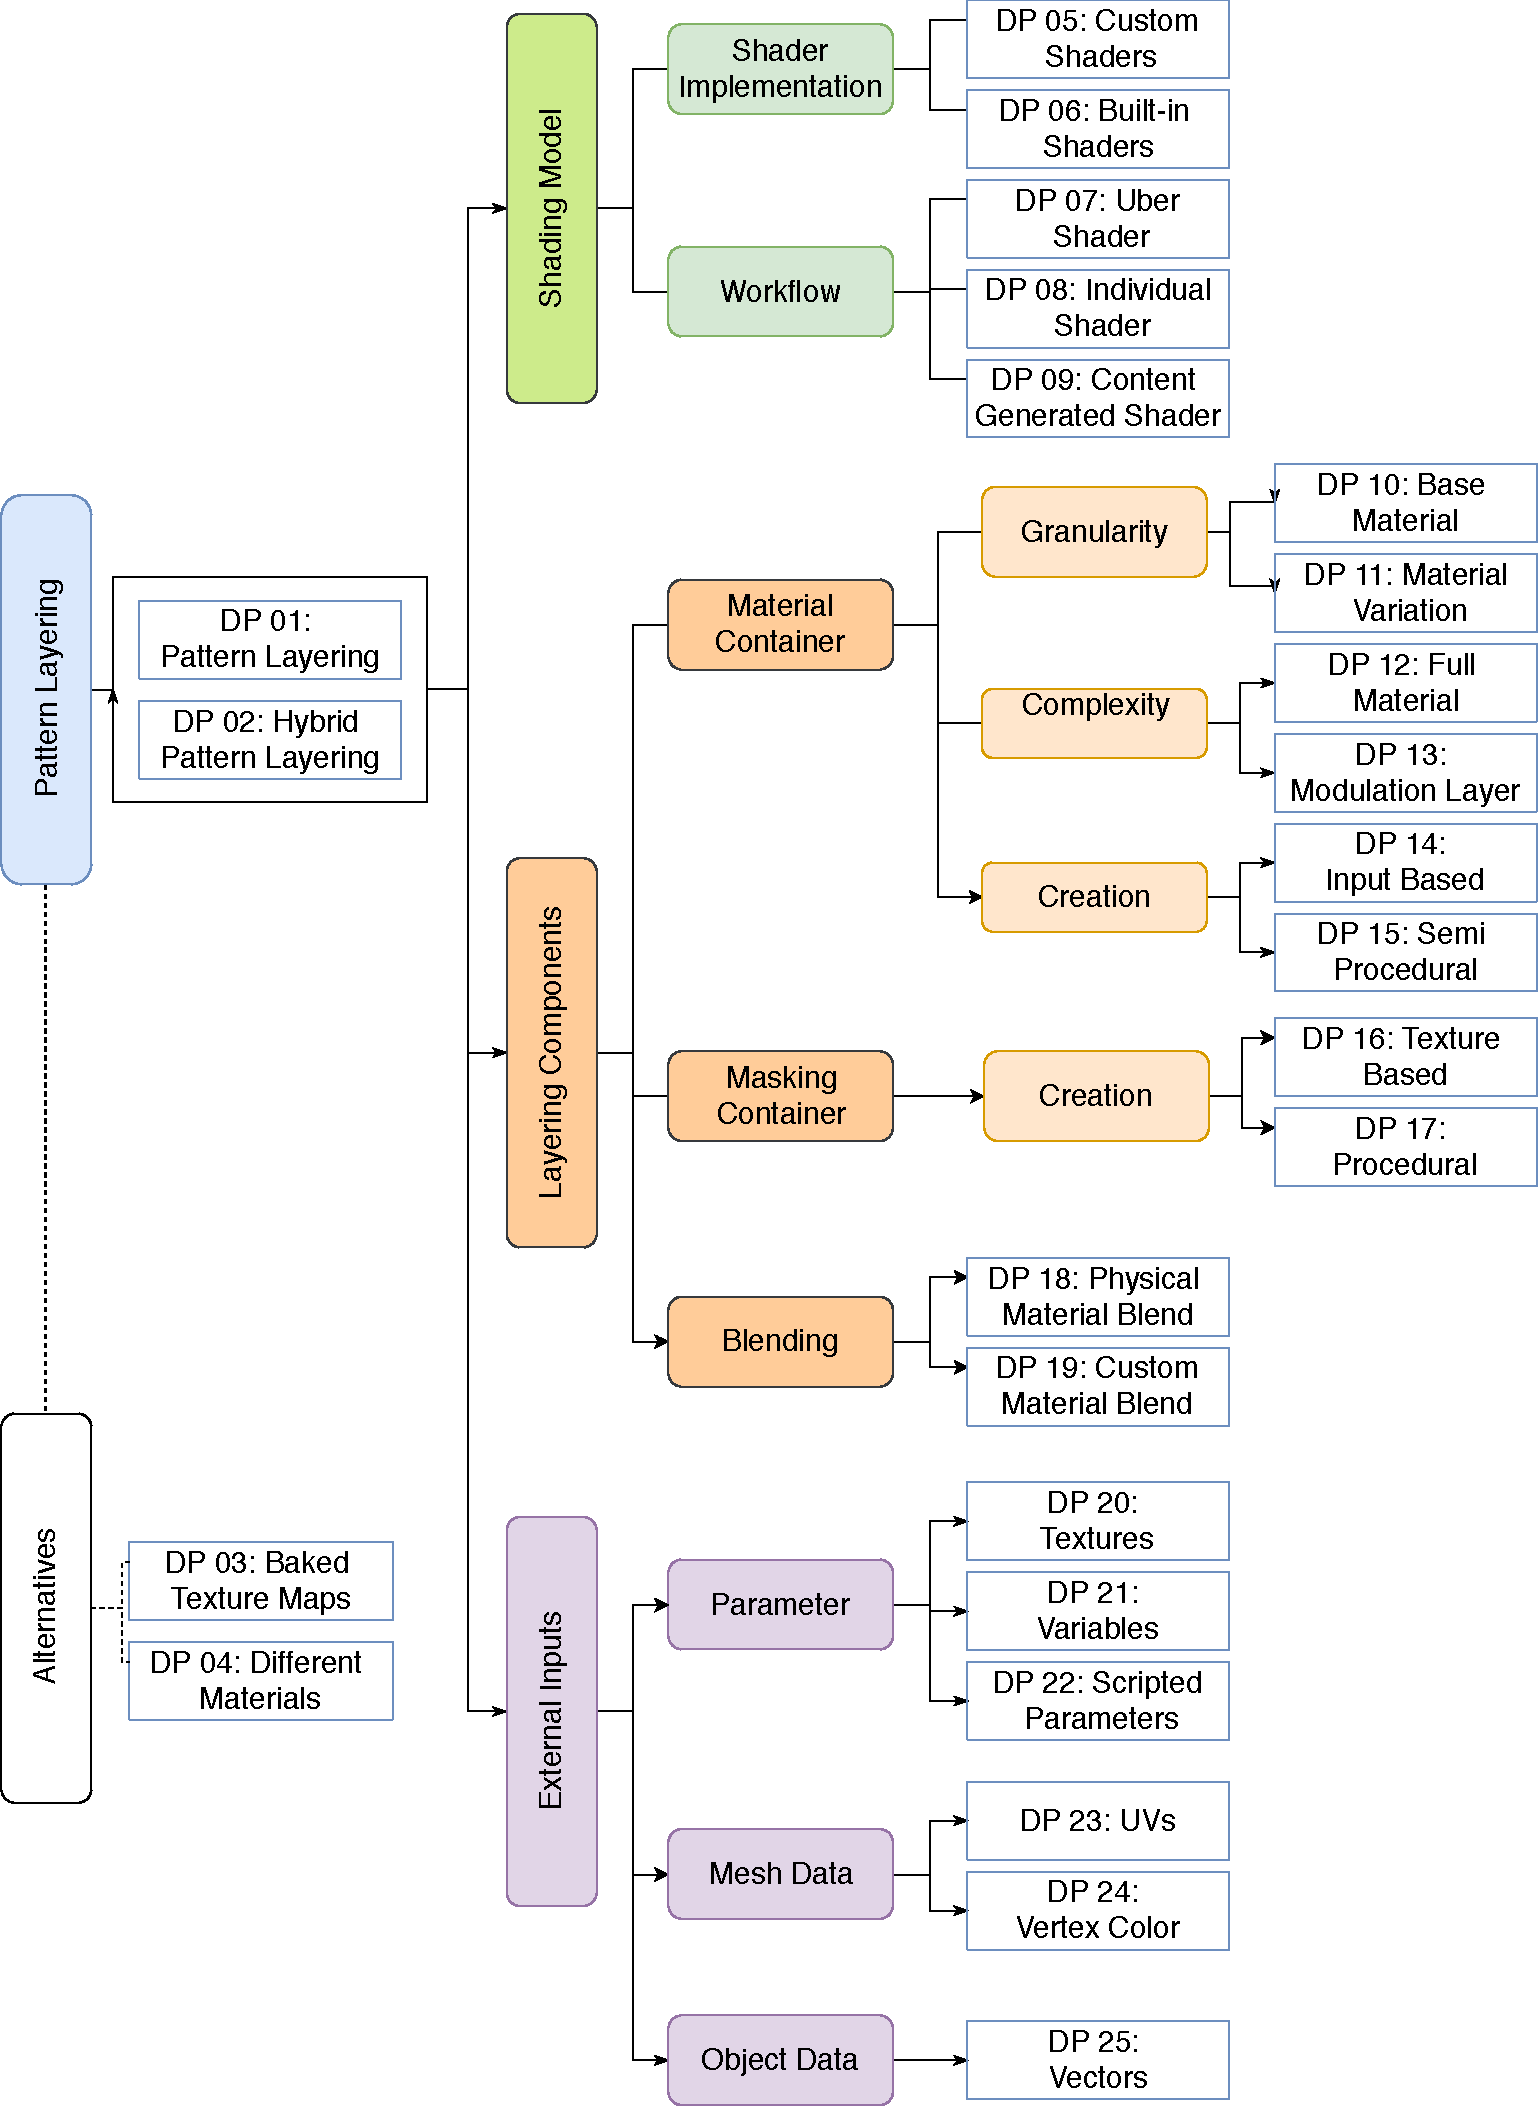
\includegraphics[width=0.7\linewidth]{images/07cha_01_PatternDesign.pdf}
	\caption{The hierarchical structure of the design patterns presented in this work. The primary element is \emph{\patTitle}. The category \emph{\patCatAlternatives} shares the same hierarchical level as it proposes equally valid alternatives. All of the other elements are descendants of \emph{\patTitle} (\emph{\patPatternLayering} and \emph{\patPatternLayeringHybrid}). The categories \emph{\patCatShaderModel}, \emph{\patCatMaterialContainer}, \emph{\patCatMaskingContainer},\emph{\patCatBlendingModule} and  \emph{\patCatExternalInputs} contain more specific and detailed patterns and progress from high level workflow and organization decisions to specific low level features.}
	\label{image:designPatternsOverview}
\end{figure}

\section{Pattern Layering}\label{sec:patternStructure}
This catalog starts off with two different approaches to include pattern layering into your workflow. Patterns \emph{\patPatternLayering} and \emph{\patPatternLayeringHybrid} present two different approaches to do so. The former introduces a pure pattern layering shading. The latter proposes a hybrid method that combines pattern layering with more traditional object specific approaches. 
These patterns in connection with the patterns in category \emph{\patCatAlternatives} will support you in taking the biggest decision connected with this pattern catalog. Does pattern layering make sense for your specific project? The second question that arises is whether pattern layering alone provides the desired result or is a hybrid approach better suited.  

\subsection{\patPatternLayering}\label{\patPatternLayering}
\begin{description}
	\item [\patIntent:]Use different generic and tileable material layers and combine them to recreate the visual appearance of complex surfaces. Built a pipeline based on re-usable components and tools (e.g., material library and parametric masking). %material library und parametric masking
	\item[\patAlsoKnownAs:] \emph{Parametric Layering}, \emph{Material Masking System (MMS)}, \emph{Layered Materials}, \emph{Material Layering}, \emph{Dynamic Material Layering}
	\item [\patMotivation:]	Consider working on a huge scene for a first person shooter. Most areas can be seen from both a further distance as well as from really close up.\,Remember the castle wall example from chapter \ref{chahpter:introduction} that was composed of many different base materials. Working with unique pre-baked texture maps would largely exceed the memory if trying to achieve a consistent high texel density.
	
	The asset and shading pipeline of the company or team you work for transitions more and more into the engine. Different artists use different tools for the texturing. The companies goal is to unify the material pipeline, create a central base material library and use advanced shading instructions (e.g., real-time tessellation, parallax occlusion mapping and vertex shader animation). These advanced shading techniques cannot be reproduced and shared across different applications easily.
	\item[\patApplicability:]\hfill 
	\begin{itemize}\mynobreakpar
		\item All base materials use the same shading model.
		\item The shading system has to account for a huge, complex surface area where different base materials are used. The transition of these base material is smooth, geometry independent and most likely on a per pixel basis.
		\item  The blending uses procedural components that respect any properties defined in the material container. For instance, both base materials are blended according to their height map so that base material \emph{B} appears only in the valleys of base material \emph{A}. 
		\item The masking and blending of the layers uses various information from the scene, such as position, normal direction and so on.
		\item The blending of different base materials is modified dynamically at runtime. Imagine peddles integrated into the material shader that respond to global weathering systems within the game. 
		\item A lot of different material variations of the same object are needed.
		\item The workflow is supposed to be iterative. Individual base materials can change independently and are easy to be replace if desired.
		\item Base materials can be used and re-used across different objects, projects and artists.
		\item The project uses a centralized art directed material library that can be shared across different artist. Changes on the base materials are propagated down to all assets using them. Working with a centralized art directed material library also improves consistency across different assets.    
	\end{itemize}
	\item[\patImplementation:] There are many different ways to implement a pattern layering (see chapter \ref{cha:implementationParametricLayering}). The user experience differs strongly according to which one is used. The different approaches to implement a pattern layering system are to use either built-in shaders (\emph{\patImplementationBUildtIn} in section \ref{\patImplementationBUildtIn}) or  create custom ones (\emph{\patImplementationCustomShader} in section \ref{\patImplementationCustomShader}). Custom shaders can be implemented using HLSL/Cg, shader graph editors or material layering systems.
	\item[\patExamples:] Most of the patterns presented in this catalog were tested within the VR experience \emph{Letzte Worte}. A lot of these patterns arose from questions I had myself throughout the project. The suggestions found in different publications, talks, articles and sample projects helped me take decisions on how to handle an individual problem. All these practical experiences flowed back into these patterns. In \emph{Letzte Worte} I used pattern layering for all environment assets except detail props like electronics, machines, books, lamps etc. \emph{Letzte Worte} uses a wide variety of different patterns presented in this catalog.  
	\item[\patConsequences:]\hfill 
		\begin{description}
			\item[\visual:]\hfill
			\begin{itemize}\mynobreakpar
				\item Pattern layering forces the artist to approach texturing in a technical way. 
				\item It allows the shading of huge interesting surface areas while still achieving lot of surface variety. By using repeating tillable base materials, this method enables a high screen-space texture resolution  while obtaining huge control over the blending. 
				\item The artistic process is limited by the layered material shader. The shader defines a big part of the visual quality. A lot of artistic choices are taken while creating it.
				\item A lot of the artistic process takes place on a shader level. To achieve the best results, a good technical knowledge is needed.
				\item The approach to texturing is more technical than using 3D painting applications. 
				\item Using a base material library supports a good art directability. All artists use the same materials. Changes on the base materials are propagated down to all assets using them. 
			\end{itemize}%
			\item[\performance:]\hfill
			\begin{itemize}\mynobreakpar
				\item Using a layered material shader can have a big impact on performance, especially depending on the complexity of the individual material layers. The real-time rendering engine computes all layers for all pixels simultaneously and blends them afterwards. Even base materials that are not visible for a certain pixel are computed \cite{epic2015LayeredMats}. 
				\item Texture memory can be decreased dramatically compared to traditional alternatives, as for instance \emph{\patAlternativeBaked} (section \ref{\patAlternativeBaked}). This is caused by the fact that texture maps can be used across different materials and the individual texture resolution can be much smaller as it is repeated multiple times over the surface area. 
			\end{itemize}
			\item[\pipeline:]\hfill
			\begin{itemize}\mynobreakpar
				\item It is hardly possible to exchange shading data with other applications. To do so often requires other custom pipeline tools.
				\item Blending individual material parameters of two material layers is not a trivial task. Either the
				pipeline or the artists have to account for the complex process of blending (e.g., roughness, ior accumulation). Please refer to section \ref{sec:blendindIssuesLayering}.				
				\item Using custom shaders may require project specific tools and systems to support an efficient workflow. See pattern \emph{\patImplementationCustomShader} in section \ref{\patImplementationCustomShader}.
				\item Creating a pipeline for material layering is time consuming. The development and testing of shaders and pipeline tools are expensive and time consuming. 
				\item Working on \emph{Letzte Worte}, I realized that using a highly customized shading workflow may cause issues with different features provided by the engine (e.g., hierarchical LODs and lightmaps).
			\end{itemize}
		\end{description}

	\item[\patRelations:] This pattern represents a pure pattern layering based shading workflow. \emph{\patPatternLayeringHybrid} (section \ref{\patPatternLayeringHybrid}) proposes a more flexible approach that includes features of other methods as well. The category \emph{\patCatAlternatives} contains alternative texturing approaches. Categories \emph{\patCatShaderModel} (see section \ref{\patCatShaderModel}), \emph{\patCatMaterialContainer} (see section \ref{\patCatMaterialContainer}), \emph{\patCatMaskingContainer} (see section \ref{\patCatMaskingContainer}),
	\emph{\patCatBlendingModule} (see section \ref{\patCatBlendingModule}),
	 and \emph{\patCatExternalInputs} (see section \ref{\patCatExternalInputs}) contain further information on how to use and implement pattern layering in your project.	
\end{description}	


\begin{figure}
	\centering
	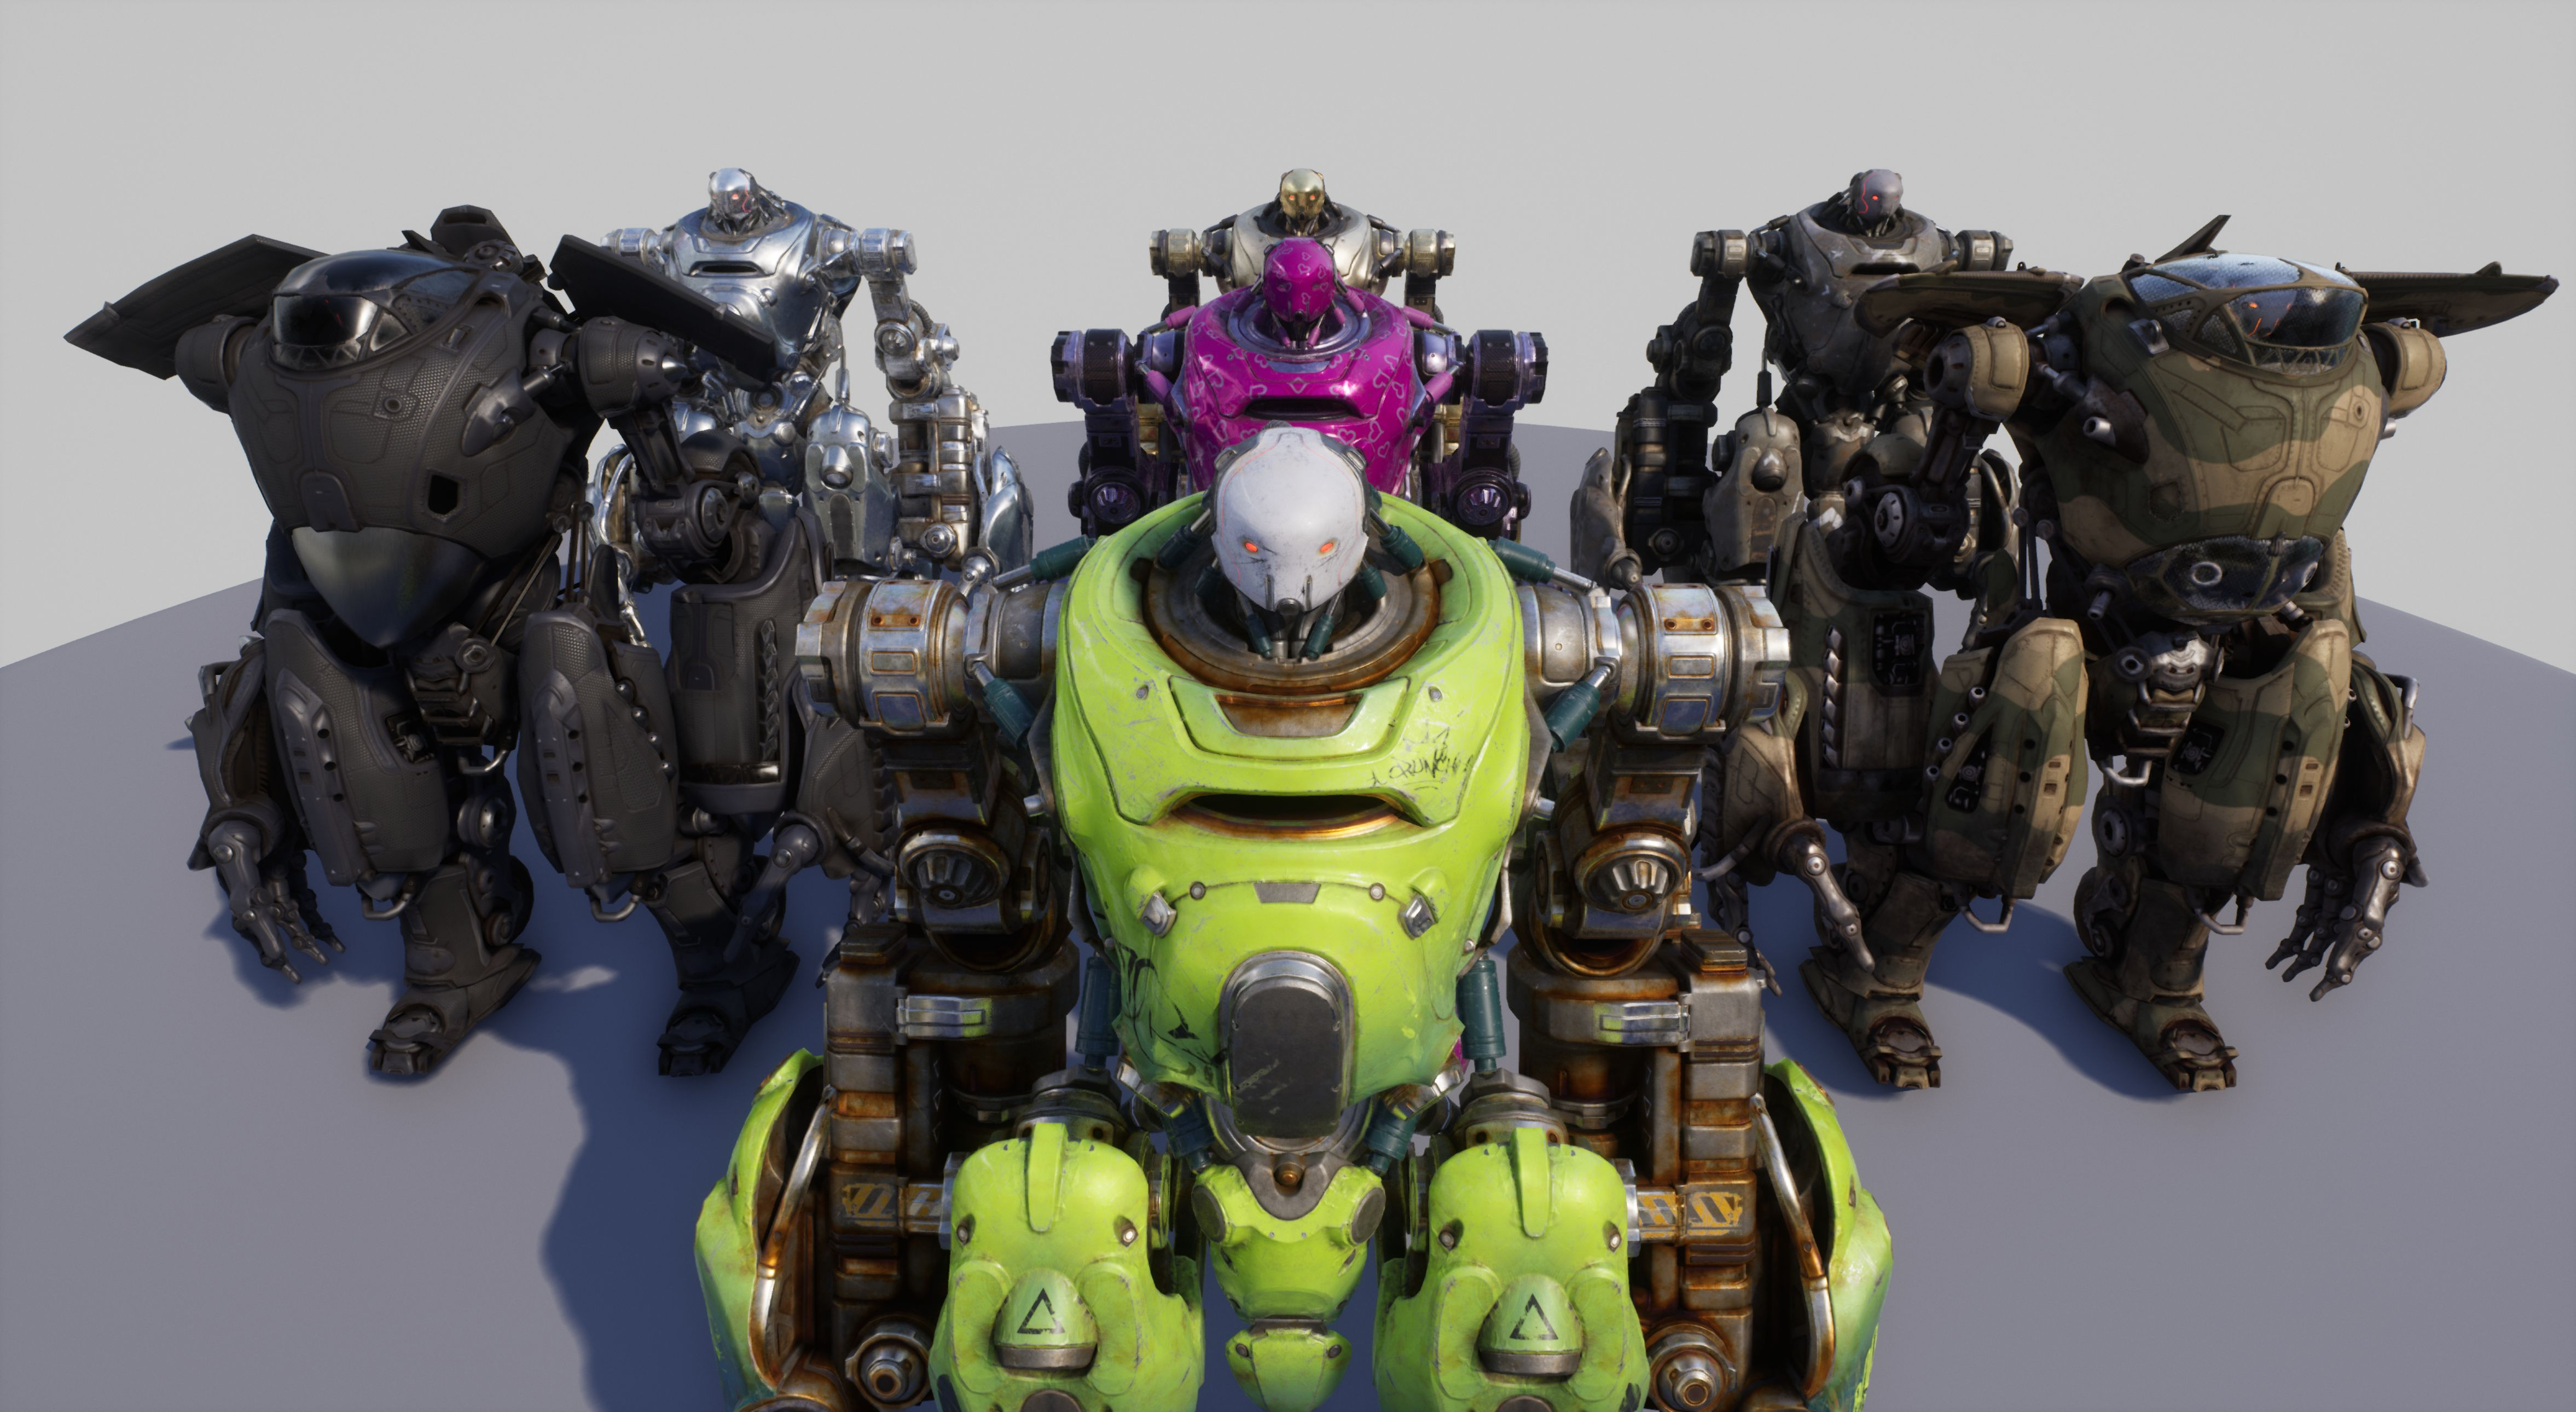
\includegraphics[width=0.9\linewidth]{images/07cha_02_MaterialLayeringVariety.jpg}
	\caption{Different skins of \emph{Chrunch}, a hero character from the \emph{MOBA} \emph{Paragon}. Pattern layering was used to quickly iterate and create variations of different skins during the production. This rendering was made by using the assets from the official \emph{Epic Marketplace} \cite{epic2018chrunch}.}
	\label{fig:materialLayeringVariety}
\end{figure}


\subsection{\patPatternLayeringHybrid}\label{\patPatternLayeringHybrid}
\begin{description}
	\item[\patIntent:]% 
	In order to create small scale details, an object specific single texture for the large scale variety and a more generic pattern layering workflow are to be combined.
	\item[\patMotivation:]% 
	Photogrammetry is a process to capture meshes and textures from real world locations and objects. The data has to be optimized and cleaned for the use in a real-time application. However, it provides high quality with less effort compared to traditional methods. The advantages and disadvantages of using these textures directly are eplained in pattern \emph{\patAlternativeBaked} (section \ref{\patAlternativeBaked}). Matching the scanned data by purely layering base materials is difficult, time consuming and expensive. Even by matching the reference, it will most probably not be practical due to the huge amount of different layers and complex masks for blending them. Therefore, this design pattern combines aspects from both methods, i.e., object specific texture maps from pattern \emph{\patAlternativeBaked} (section \ref{\patAlternativeBaked}) with additional generic, tileable and reusable base materials as explained in pattern \emph{\patPatternLayering} (section \ref{\patPatternLayering}).
	\item[\patApplicability:]\hfill
	\begin{itemize}\mynobreakpar
		\item The object fits all criteria for being shaded by using a pattern layering approach, but additional large scale information (e.g., photoscanned textures) is available. 
		\item The artistic goal is not achieved by combining different generic base materials. Additional object specific large scale variety is needed. 
	\end{itemize}
	\item[\patImplementation:]%
	The hybrid pattern layering shares the same technical implementation as other layered material methods. In the context of the material layering model established in chapter \ref{cha:partsOfLayeredShader}, the additional object specific texture maps can be seen as individual arbitrary material container. On the implementation level, it can be treated like any other material container outputting an material layer object. Finally, different blending modes can be used to add to the final shading output. %TODO implementation unity layered shader
	\item[\patExamples]%
	Figure \ref{fig:layerdLitUnity} shows an example using pattern layering combined with object specific photogrammetry textures  \cite{unity2017photogrammetryLayered}. This example illustrates that combining real world captured object specific textures with pattern layering can be used to achieve realistic results. It further allows reusing and sharing tileable base materials across different assets. As shown in the image, this technique allows to easily create different variations and supports an iterative workflow.   		
	\item[\patConsequences]% 			
	Hybrid pattern layering is identical to \emph{\patPatternLayering} (section \ref{\patPatternLayering}) from a technical perspective. The additional object specific textures do provide some artist friendly possibility for adding large scale variety. These texture maps are not ideal to add small scale details as this would require huge texture resolutions and therefore eliminate the advantages of \emph{\patPatternLayering} over \emph{\patAlternativeBaked}.  
	\item[\patRelations]%
	This pattern combines aspects of \emph{\patPatternLayering} (section \ref{\patPatternLayering}) and more traditional methods like \emph{\patAlternativeBaked} (section \ref{\patAlternativeBaked}).
\end{description}


\begin{figure}
	\centering
	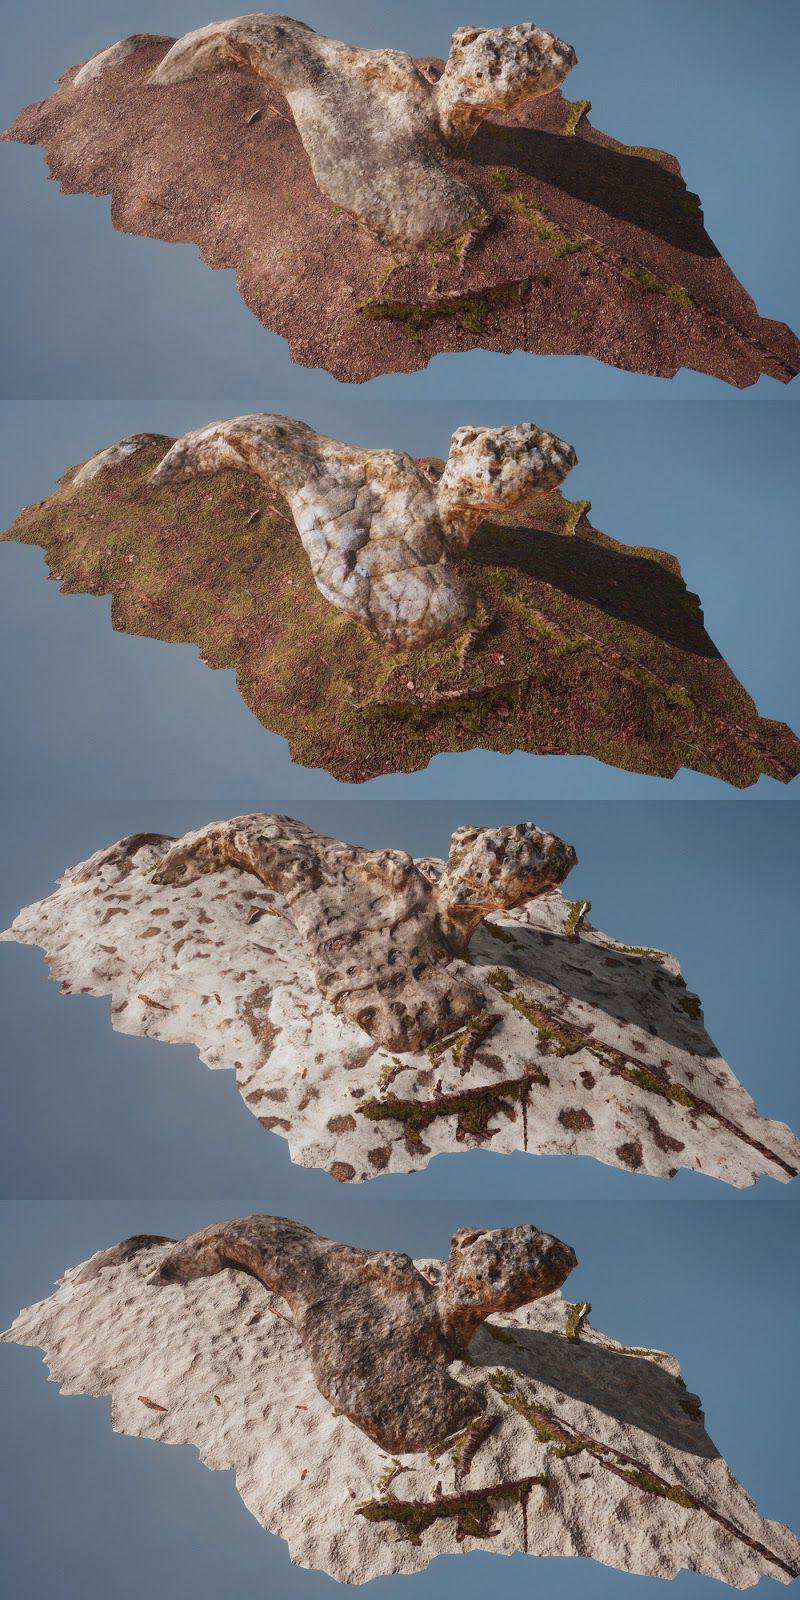
\includegraphics[width=0.65\linewidth]{images/07cha_03_layeredLitUnity.jpg}
	\caption{Combining 3D scanned texture data with smaller, generic and tileable base materials. This approach makes it possible to obtain the large scale texture variety captured from the real world object while ensuring a high texel density using Pattern Layering. Using pattern layering allows to easily and quickly create variations. Image source: \cite[p.\,6]{unity2017photogrammetryLayered}.
	}%END CAPTION
	\label{fig:layerdLitUnity}
\end{figure}


%%%%%%%%%%%%%%%%%%% ALTERNATIVES %%%%%%%%%%%%%%%%%%%%%%%%%%%%%%%%%%%

\section{\patCatAlternatives}\label{\patCatAlternatives}

Before going over to how design and implement a pattern layering system, I want to show alternative approaches to texturing and shading your objects. The Patterns \emph{\patAlternativeBaked} (section \ref{\patAlternativeBaked}) and \emph{\patAlternativeDifferentMatierals} (section \ref{\patAlternativeDifferentMatierals}) % and \emph{\patAlternativeTrim} (section \ref{\patAlternativeTrim})
contain workflows that are not necessarily associated with material layering. Nevertheless, they might be better suited for the particular requirements. Sometimes different approaches can be mixed as well (e.g., \emph{\patPatternLayeringHybrid} in section \ref{\patPatternLayeringHybrid}).

Other material layering approaches that might gain importance in the future are BxDF layering (see section \ref{sec:BxDFLayering}) and illumination lobe based layering (see section \ref{sec:illuminationLobeLayering}). To the best of my knowledge, pattern layering is the only material layering approach actively used for video game productions yet. Technologies like real-time ray tracing are most likely going to take over. They will change many workflows used nowadays; one of them will be the way how we handle material layering. I believe that BxDF layering (see section \ref{sec:BxDFLayering}) and illumination lobe based layering (see section \ref{sec:illuminationLobeLayering}) will replace many use cases for pattern layering. This will be a huge game changer. As discussed in chapter \ref{cha:materialLayering}, both techniques provide huge advantages as regards realism and usability. Another approach to realize material layering could be color layering (see section \ref{sec:ColorLayering}). This could be achieved by rendering multiple versions of the object and save the outputs in additional buffers. The data could be blended together in the post-processing stage. This approach is expensive in computation and memory. Further experimental investigation needs to be done on this subject to see if there are any use cases for this approach. 




%%%%%%%%%%%%%%%%%%%%%%%%%%%%% Alternatives  %%%%%%%%%%%%%%%%%%%%%%%%%%%%%
\subsection{\patAlternativeBaked}\label{\patAlternativeBaked}
\begin{description}
	\item[\patIntent:]%
	Use a pre-baked object specific single textures for the individual material inputs (e.g., base color, normal and roughness) to define the object appearance in the final render. Using object specific textures provides the most control over the final appearance on a per pixel basis. 
	%\item[\patAlsoKnownAs]%
	\item[\patMotivation:]%
	Consider an object with a huge variety of different base materials. The surface appearance is heterogeneous and it is really difficult to identify distinctive base materials. This makes it difficult to recognize recurring patterns in masks and base materials and recreate the surface by combining more generic base materials.
	
	The specific asset plays a major role for either the gameplay or the plot of the game. Therefore, the most artistic control is required. You are working on small detail props for an office desk. These different assets (e.g., pencil, hole puncher, paper clip and post-it note) are composed of many different base materials. The list of base materials might look similar to this: rubber, plastic wood, painted wood, aluminum and paper. These different base materials do have additional variations. So for instance, there is a red and a blue pencil. The amount of base materials for texturing these assets with \emph{\patPatternLayering} (section \ref{\patPatternLayering}) is extremly high. As these assets are fairly small, they do not need a big texture resolution to achieve a high texel density. Additionally, this pattern is not limited by the amount of surface type variety in any way. It does not matter if a single texture represents one or fifty surface types. 
	\item[\patApplicability:]\hfill
	\begin{itemize}\mynobreakpar
		\item A low texture resolutions is enough to achieve a high screen-space texture resolution for the desired object. The necessary texture resolution does not necessarily refer to the dimensions within the 3D scene but to the maximum screen-space the object covers. A huge mountain located in a far distance can be textured by low res textures and still have sufficient screen-space texture resolution. A wall seen from close may exceed the screen size multiple times and therefore need a much higher texel density.
		\item The used base materials are specific to this particular object. The surface appearance cannot or hardly be recreated by combining more generic base materials. 
		\item The surface area of this object is heterogeneous and composed of a huge amount of different surface materials. Splitting it into layers would result in a huge amount of different base materials and masks. 
		\item This object has a special significance for the experience and the maximum amount of artistic control on a per pixel basis is required. 
	\end{itemize}  
	\item[\patImplementation:]%
	Using baked texture maps is probably the most artist friendly shading workflow within 3D real-time applications. This workflow has existed for a long time, the tools and workflow have been highly simplified and optimized. This applies for both usability and performance. Most modern creation tools provide a workflow where you immediately see an output close to the final product. Artists coming from other fields can easily adapt to 3D painting tools, as they are structured similar to \emph{Photoshop}. Especially since PBR has become a well established standard, textures for the individual material inputs can easily be shared and transfered throughout a pipeline. Content creation applications and real-time engines do offer pre-existing shaders that have already been set up. The user does only need to assign the textures to the proper material slot. Modern tools like \emph{Substance Painter} eliminate much of prior shortcomings in texture painting applications. For instance, \emph{Substance Painter} provides the possibility to simply increase the texture resolution even beyond the painting resolution. It enables the artist to paint and work on several textures simultaneously (e.g., base color and roughness). It provides pre-defined export presets to convert textures for the desired render engine, i.e., it adjusts the roughness curve to correspond to the specular algorithm used in the renderer.
	\item[\patExamples:]% 
	\emph{Letzte Worte} uses baked texture maps for all the detail assets. These assets are composed of many different surface types. Using pattern layering would result in an enormous amount of different base materials as well as their variations. These assets are small enough to achieve a high texel density even by using medium texture sizes. By combining a lot of these assets into one texture atlas and using textures compression, texture streaming and channel packing,\footnote{Channel packing refers to the process of combining different textures into one by saving them into different color channels.} the memory usage is still highly efficient. Additional details that require even more detail (e.g., fonts, symbols, labels) use an additional UV set that provides the resolution where it is needed.
	\item[\patConsequences:]\hfill 
		\begin{description}
			\item[\visual:]\hfill
			\begin{itemize}\mynobreakpar
				\item Using pre-baked textures provides the highest artistic control on a per pixel basis. 
				\item It allows the use of an infinite amount of different surface types. There are no limitations on surface variety within the capabilities of the shader.   
				\item Textures can be unique for every material.
				\item It is difficult to achieve a consistent art style across different artists and assets. 
			\end{itemize}
			\item[\performance:]\hfill
			\begin{itemize}\mynobreakpar
				\item This method uses only a low amount of inputs. When packing different assets into texture atlases and using channel packing the amount of draw calls can be reduced. 
				\item The engine provides many optimizations for handling textures like mid mapping, compression and texture streaming. The texture data gets only loaded when it is needed. 
				\item The textures provide a lookup table containing complex surface descriptions. This information can be passed on to the shader without further computation. This keeps the shader complexity low even for complex surfaces. 
				\item A big amount of high texture resolutions can cause a bottleneck on the VRAM which effects performance negatively. 
			\end{itemize}
			\item[\pipeline:]\hfill
			\begin{itemize}\mynobreakpar
				\item Baked textures are well integrated in different 3D applications. 
				\item It is easy to transfer texture data across different applications. As most modern software uses a PBR system, textures can be shared quite easily.   
				\item Textures are often object-specific, and therefore they can not be reused across different meshes. 
				\item Changing the texture data means to re-export and import the maps from the texturing application to the game engine. 
				\item A lot of production effort is put into guaranteeing a consistent quality and look across different assets. 
				\item Creating object variations requires multiple textures.   
			\end{itemize}
		\end{description}
	\item[\patRelations:]% 
	This pattern proposes an alternative to pattern layering, \emph{\patPatternLayering} (section \ref{\patPatternLayering}). A combination of both methods results in a hybrid form further explained in pattern \emph{\patPatternLayeringHybrid} (section \ref{\patPatternLayeringHybrid}).
	
\end{description}


\begin{figure}
	\centering\small 
	\begin{tabular}{@{}cc@{}}
		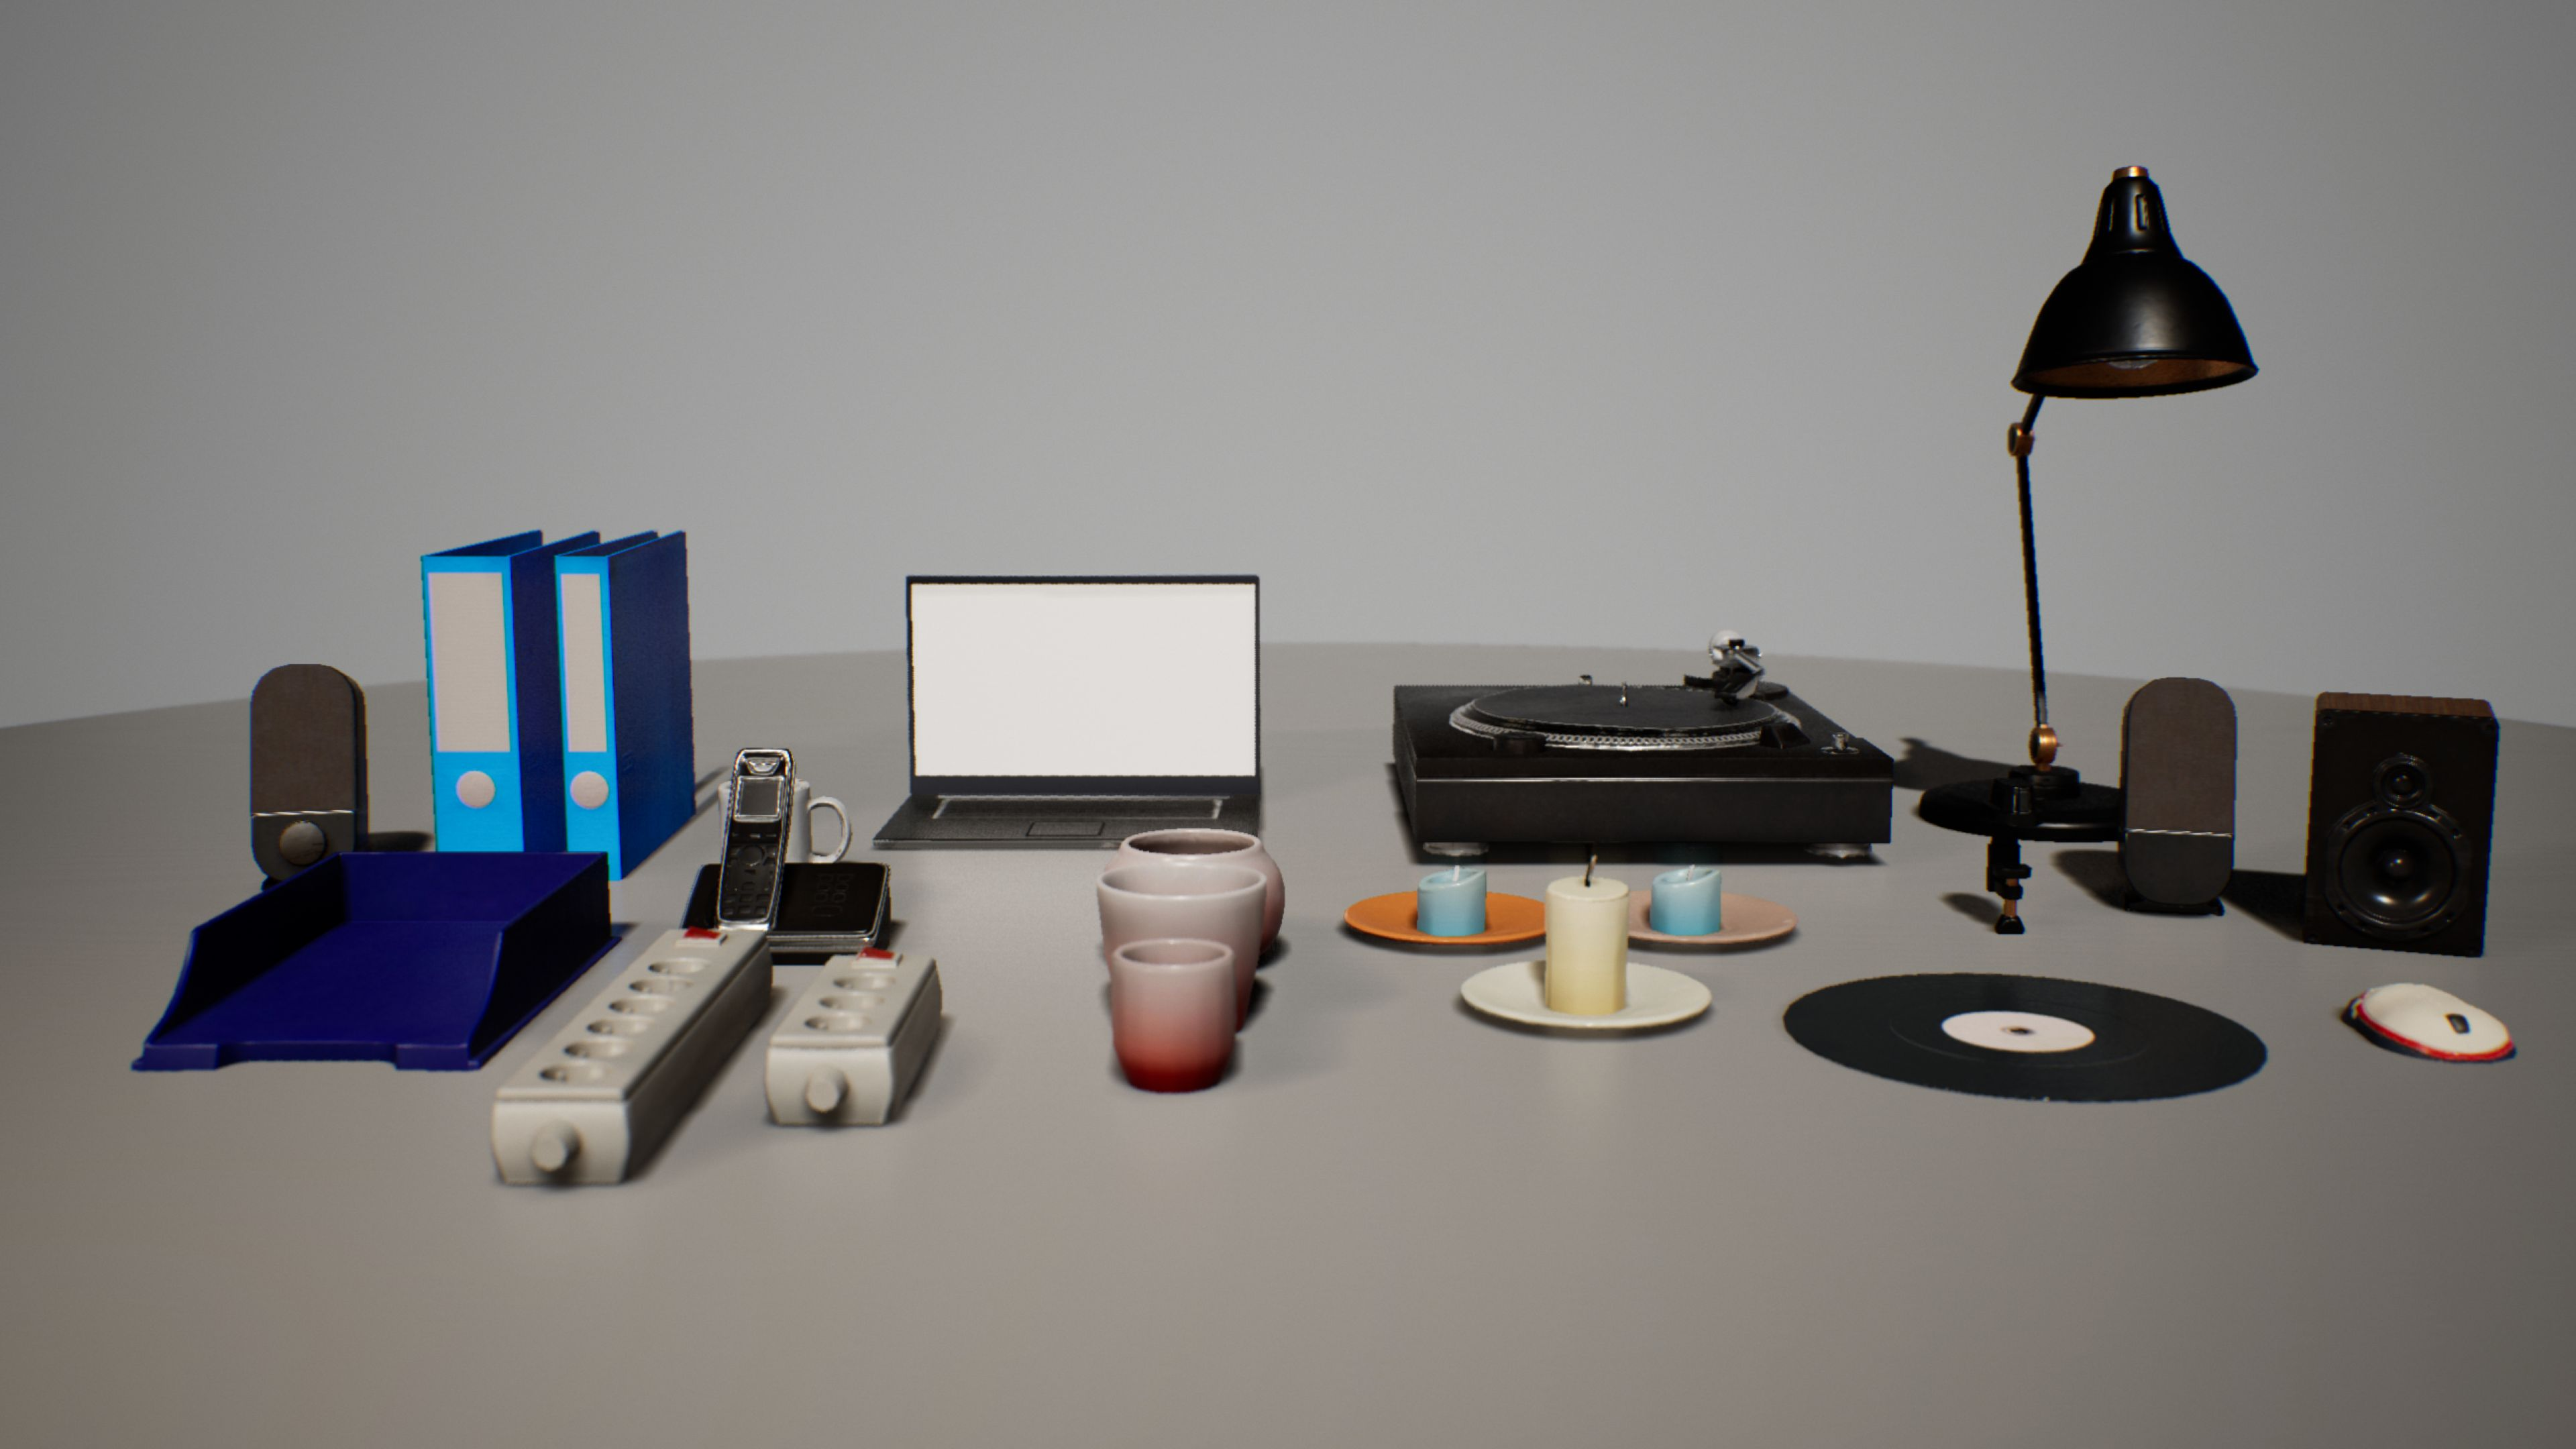
\includegraphics[width=0.575\textwidth]{images/07cha_04_pattern_LeaAssets.jpg} &
		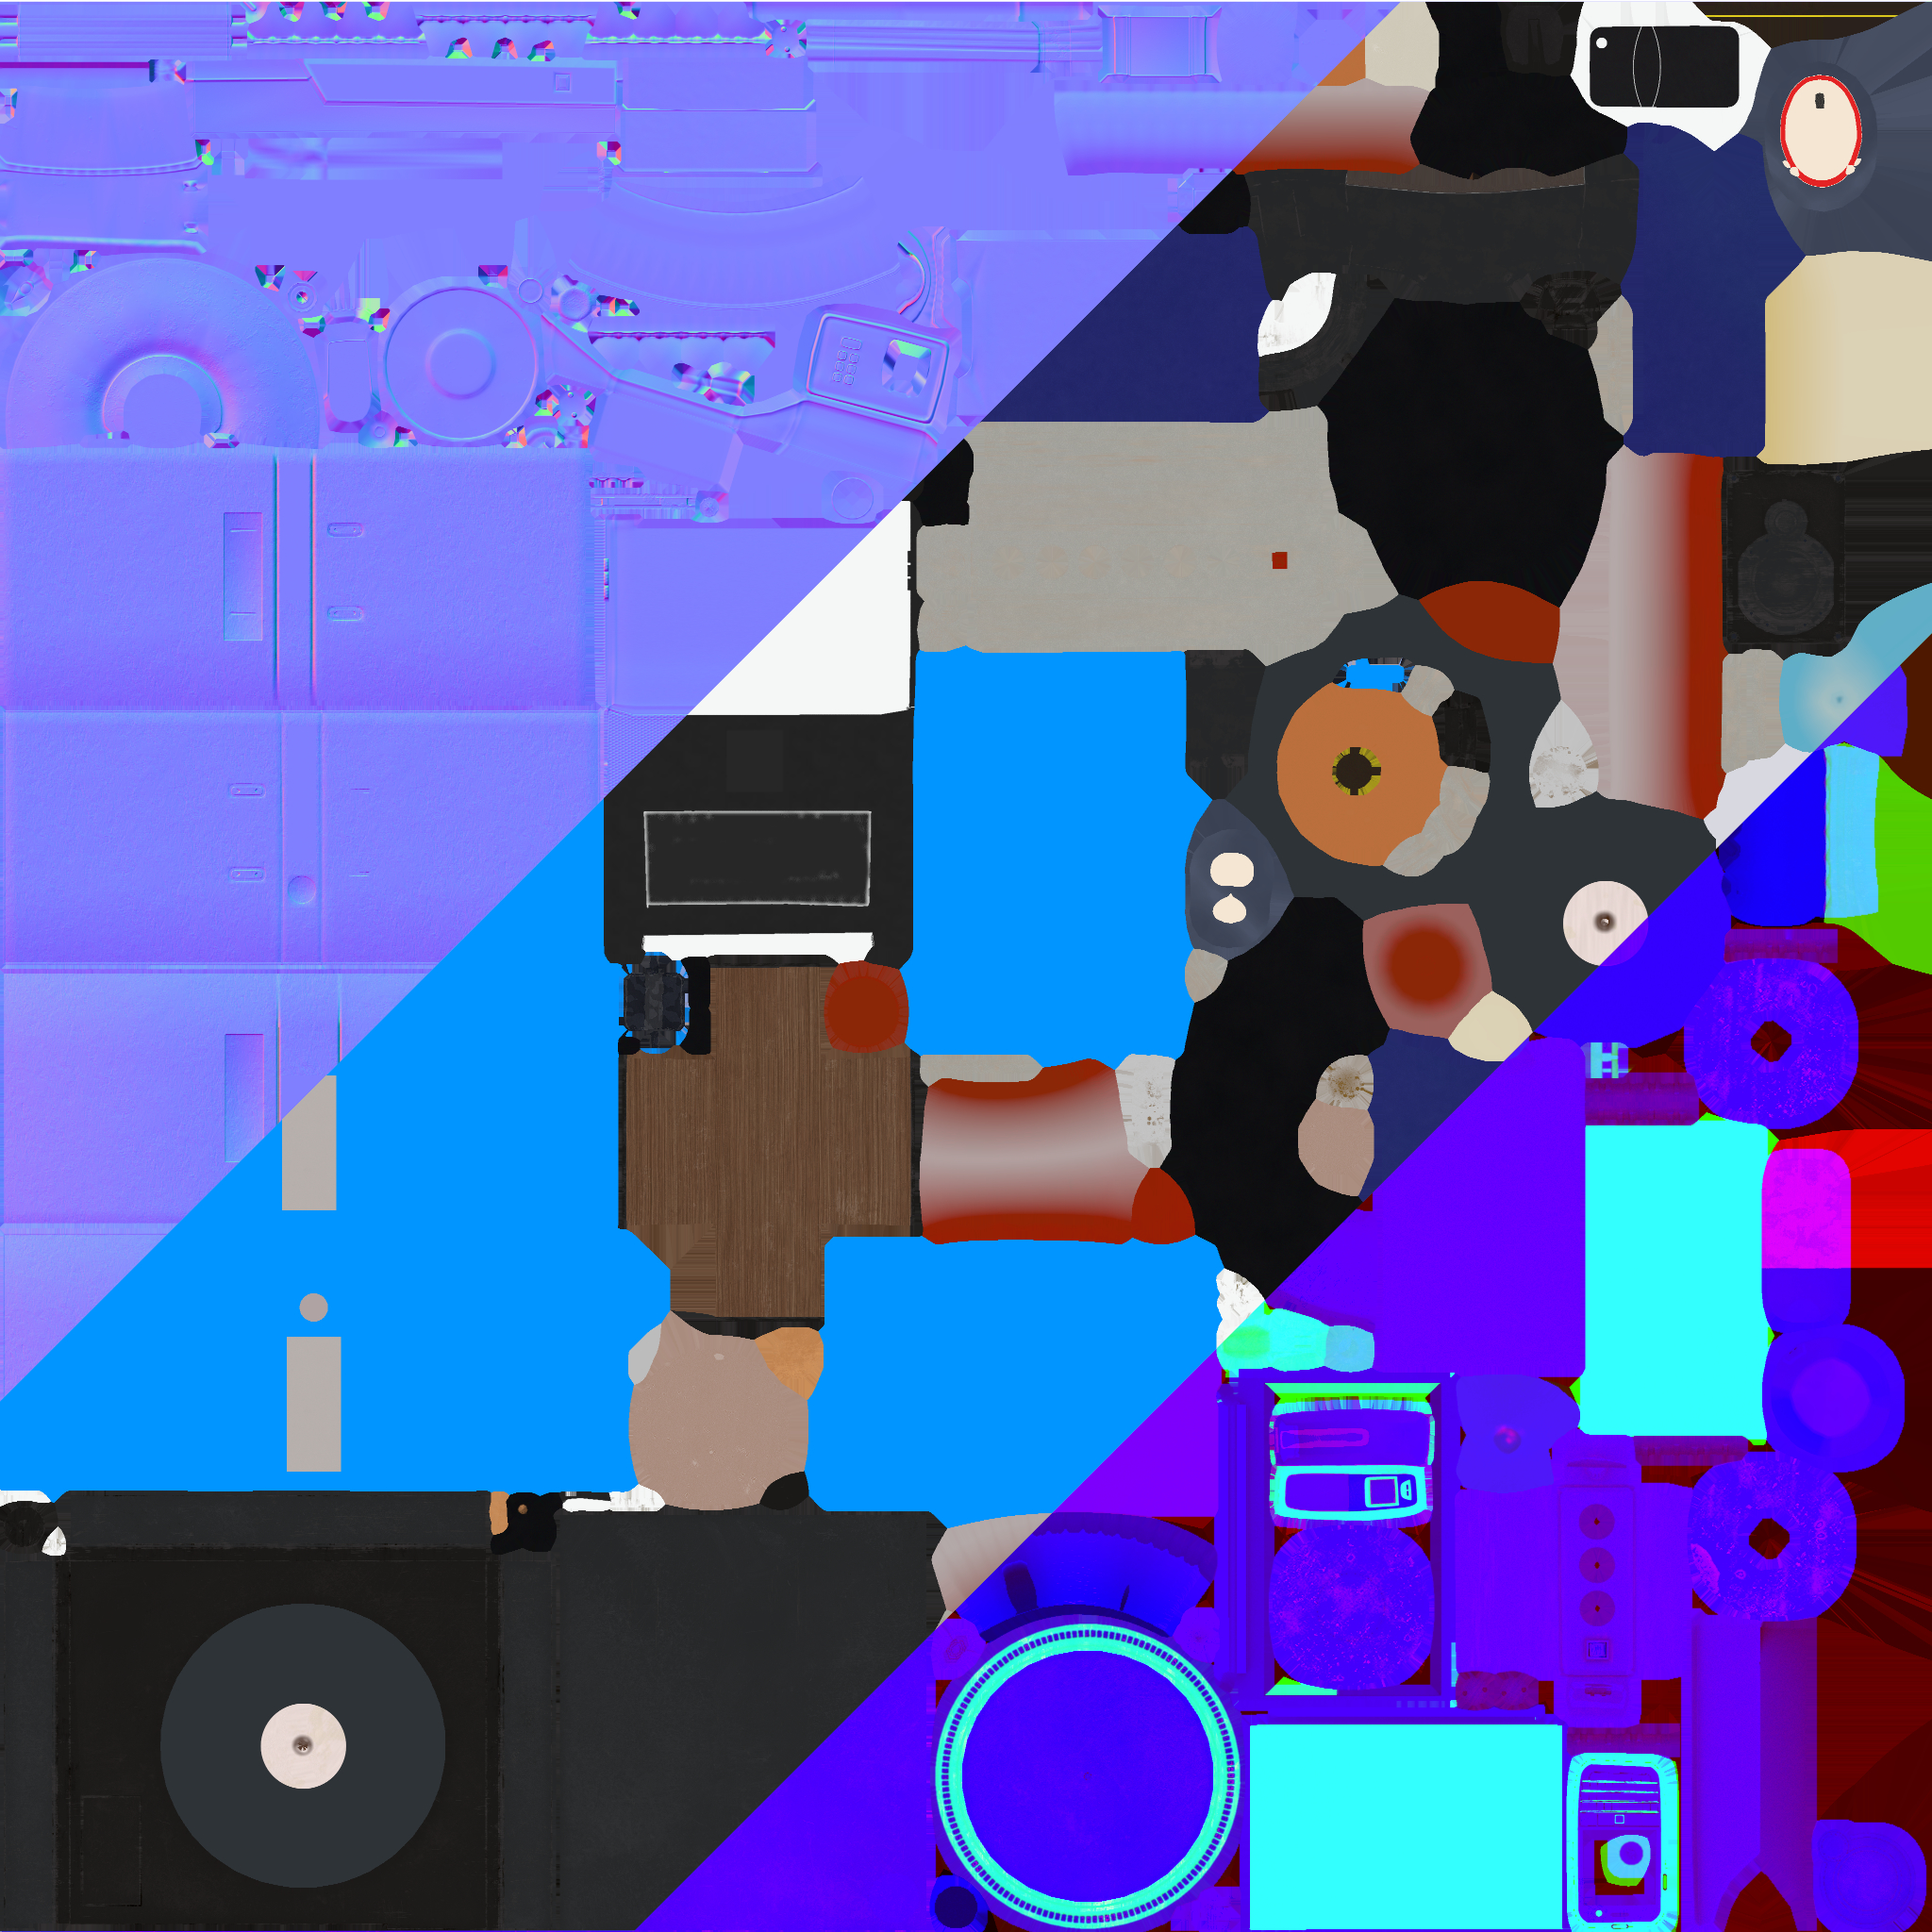
\includegraphics[width=0.375\textwidth]{images/07cha_04_textureAltas.jpg} \\	
		(a) & (b) \\
	\end{tabular}
	\label{fig:leaProps}
	\caption{Different assets using pre baked textures. The assets from figure (a) are from the game \emph{Letzte Worte}. The textures are combined into a texture atlas to minimize draw calls. Figure (b) shows the texture atlases for the following maps: the normal map, base color and a channel packed texture (roughness, metalness and ambient occlusion). }
\end{figure}


\begin{figure}
	\centering\small 
	\begin{tabular}{@{}cc@{}}
		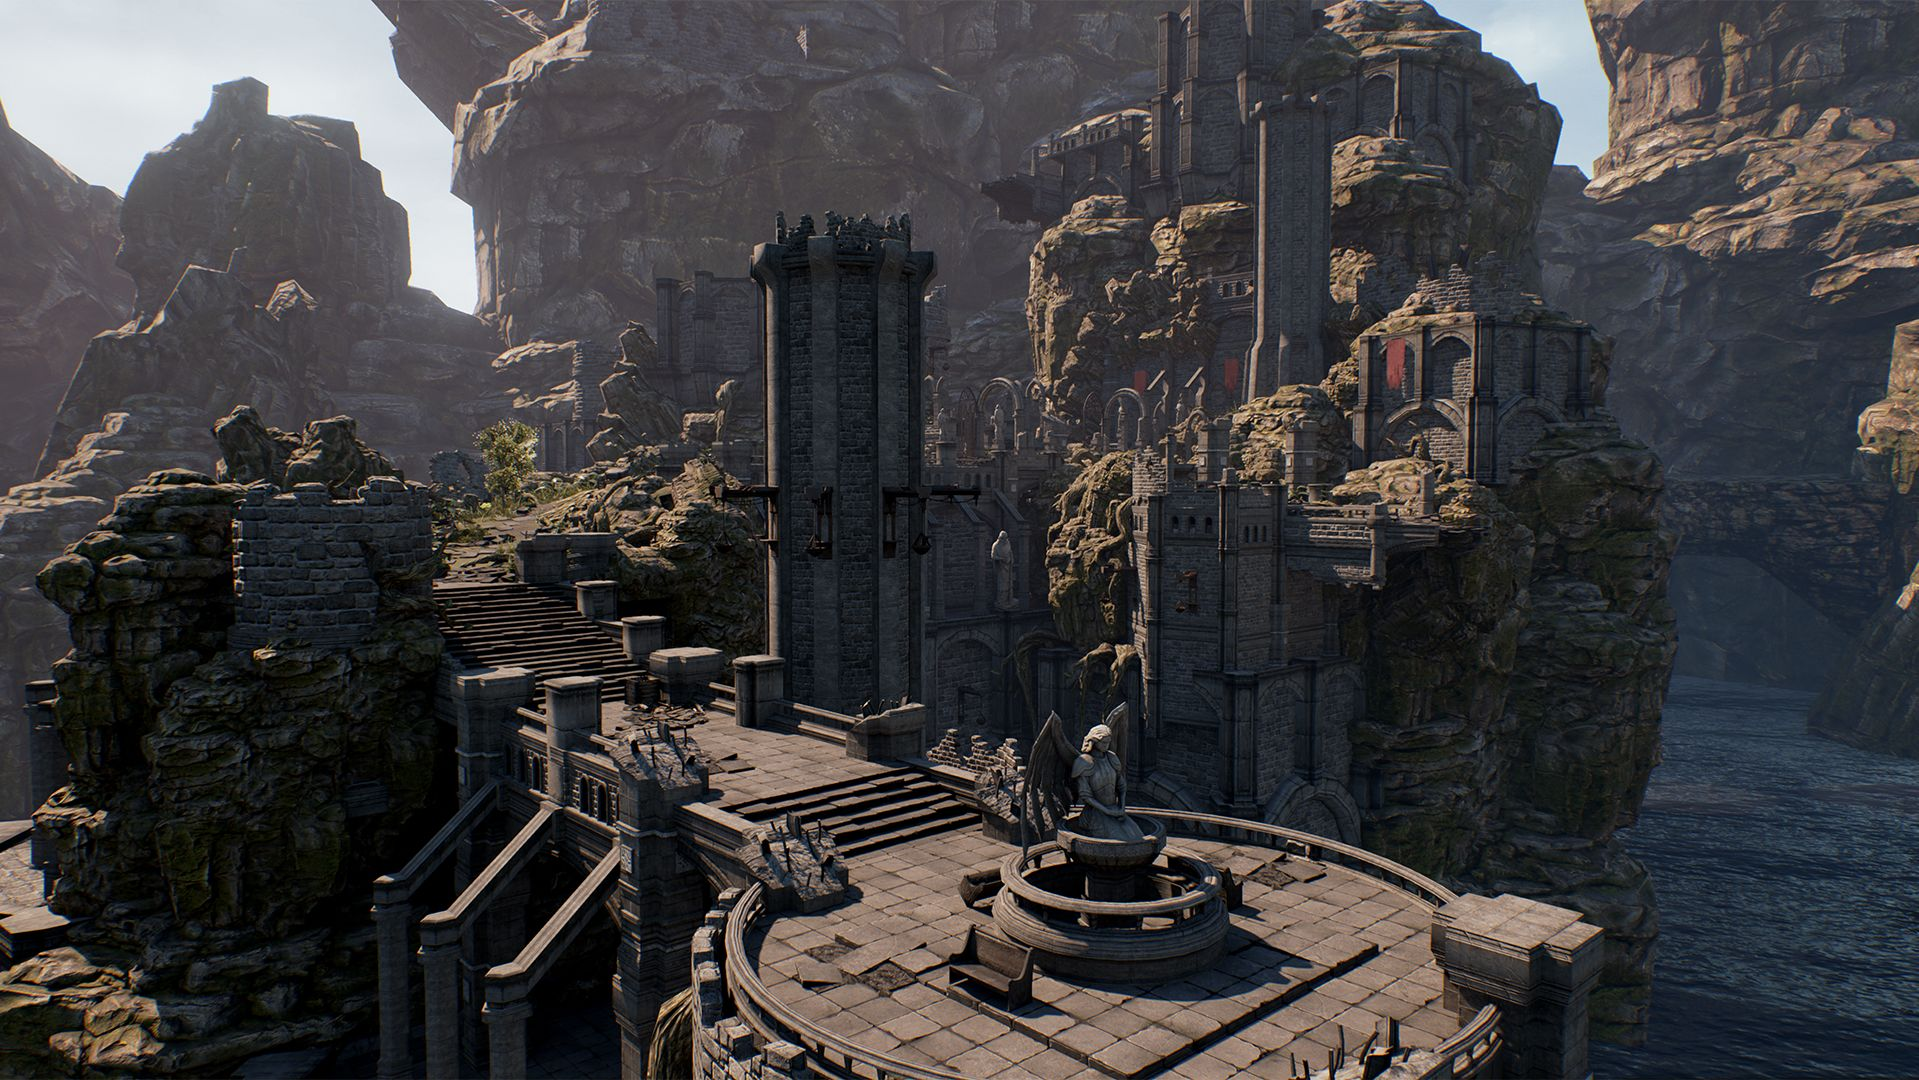
\includegraphics[width=0.475\textwidth]{images/07cha_05_pattern_TrimDivinity_1.jpg} &
		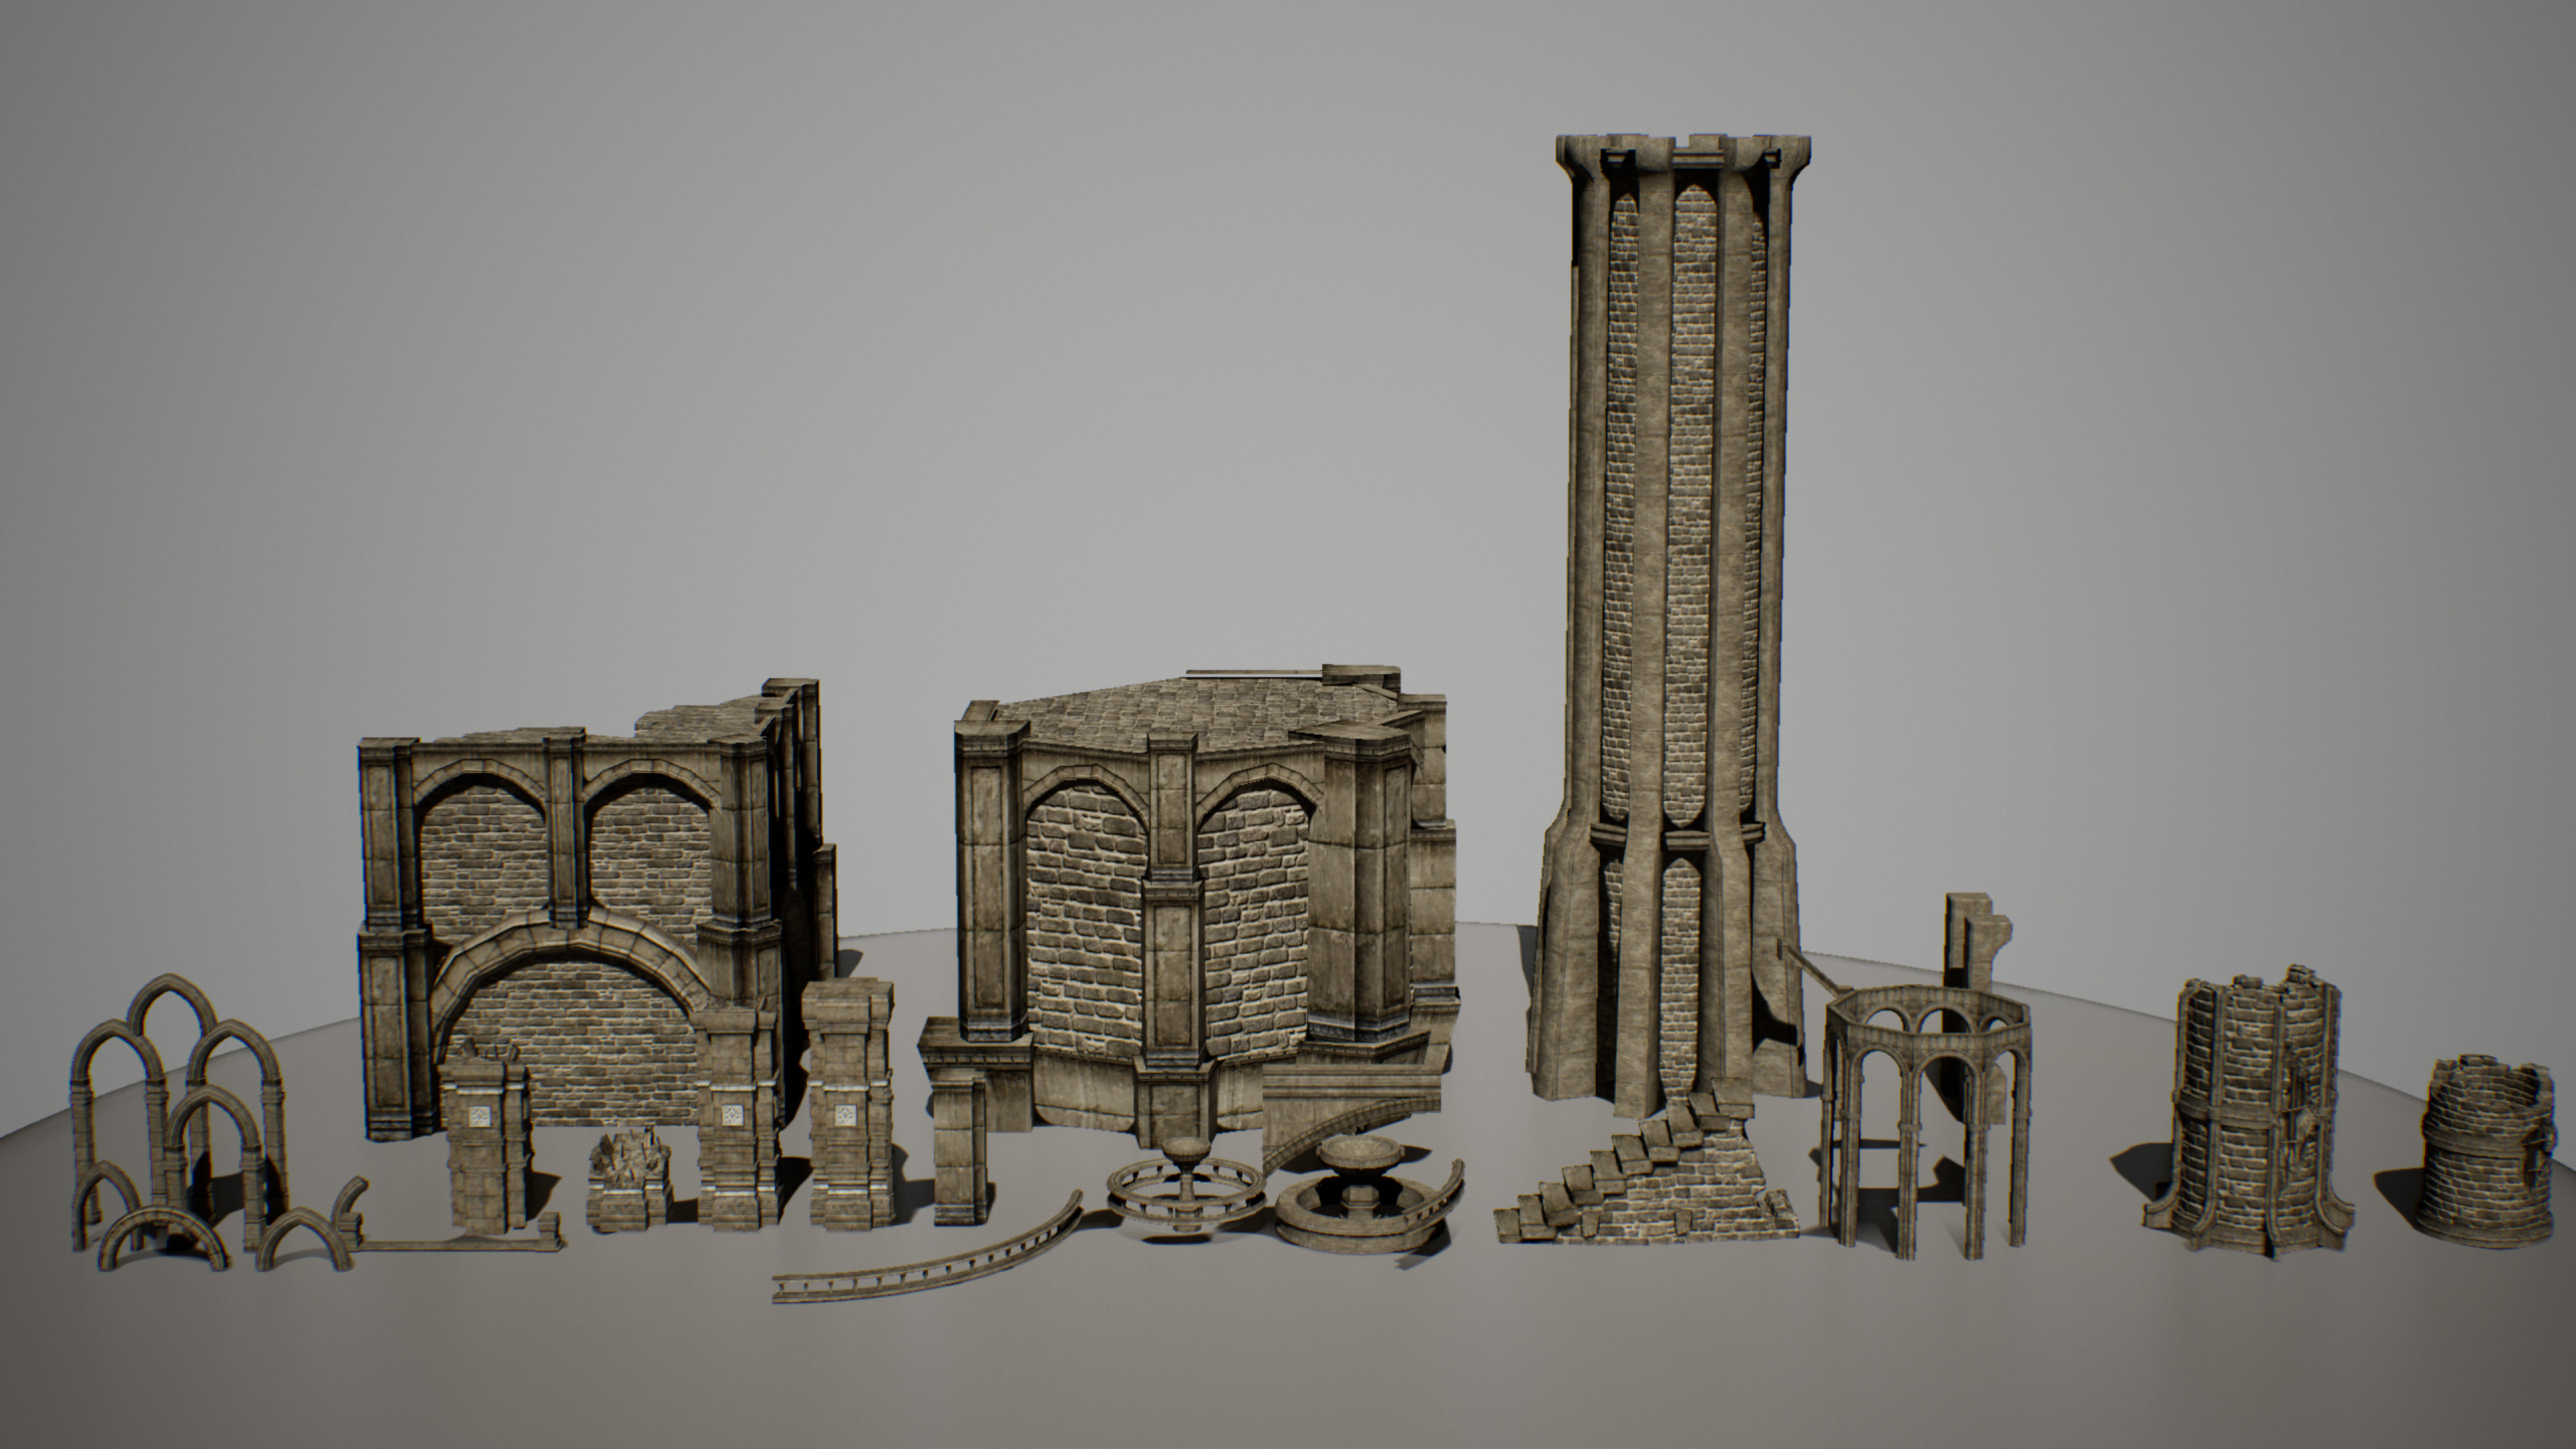
\includegraphics[width=0.475\textwidth]{images/07cha_05_pattern_TrimDivinity_02.jpg} \\	
		(a) & (b) \\
	\end{tabular}
	\caption{ 
		Scene and assets from the \emph{Infinity Blade: Grass Lands
		} map \cite{epic2018infinity}. Figure (a) shows the final scene. Figure (b) shows a selection of used assets. These assets use the same materials, a tileable wall materials and a material using trim sheet textures. The latter is used to texture details like the columns and the railings. Image source: \cite{epic2018infinity}.
	}% End caption
	\label{fig:TrimDivinity}
\end{figure}

\subsection{\patAlternativeDifferentMatierals}\label{\patAlternativeDifferentMatierals}
\begin{description}
	\item[\patIntent:]%
	Assign different materials to distinctive parts of the mesh to split the shading into individual sub-tasks. These isolated materials can be assigned to different shaders and  use different inputs. They are completely independent from one another.   
	%\item[\patAlsoKnownAs] 
	\item[\patMotivation:]%
	Consider a big architectural environment asset like a huge house. The object is composed of different distinctive areas like walls, roofs and windows. By splitting them into individual parts, material specific textures and shaders can be used. While the windows use transparency, the roof might incorporate fuzz shading for some mossy areas. Finally, the wall shader might use pattern layering and utilize vertex colors to provide more control over blending the distinctive base materials within the engine. 
	\item[\patApplicability:]\hfill
	\begin{itemize}\mynobreakpar
		\item The object can easily be divided into isolated areas representing different, distinctive surface types. The individual shader can utilize pattern layering or any other shading approach like pre-baked textures. The important requirement is that the separation between the materials uses a clear cut. It is not possible to create a smooth transition from one material to the other. By utilizing advanced shading techniques (e.g., world space UV coordinate, distance based normal interpolation or transparency), it is possible to make the transition appear smooth. Nevertheless, they are still two distinctive materials. Different materials are assigned on a per face basis; the mesh topology defines where a change in material can take place. 
		\item Different parts of the object are highly different from a shading perspective and more flexibility in changing or modifying individual areas is needed.
		\item Generic, reusable materials can be used to define certain areas of the mesh. The material does not contain object specific data. 
		\item The object is too complex or big to use one single material. 
		\item The mesh uses different shading models for different areas, such as for example opaque, translucent and subsurface scattering.
	\end{itemize}
	\item[\patImplementation:]% 
	Different material IDs can easily be assigned to an object from within the 3D content creation application. The engine can use these IDs to assign engine materials to them. Guides on how to export and import meshes with corresponding material IDs can be found in the documentations\footnote{See \url{https://docs.unrealengine.com/en-us/} for \emph{UE4} and \url{https://docs.unity3d.com/Manual/index.html} for \emph{Unity}.} of both real-time engines.
	\item[\patExamples:]% 
	Splitting objects into different materials is a common technique seen in almost any game. A particular example for utilizing different materials to shade a scene is the \emph{2014 Soul} \cite{soultechdemo2014} demo, see figure \ref{fig:soulscene}. The location \emph{Soul: City} can be downloaded from the \emph{Unreal Marketplace}.\footnote{\emph{Epic} published the map \emph{Soul:City} \cite{epic2018soul} of their \emph{2014 Soul demo} on the Unreal Marketplace (see \url{https://www.unrealengine.com/marketplace/soul-city}).} Figure \ref{fig:multiMatsSoul} shows one of the environment assets. It uses 5 different materials, each to shade a distinctive surface type. These materials are stored in a material library and are reused across all the different city assets. Different city assets are merged together to further minimize draw calls. In this particular example, the material count stays similar as the assets use the same materials. Figure \ref{fig:multiMatsSoul} shows one combined asset from the example files. By reusing the materials and merging the assets, the amount of render jobs sent to the GPU decreases dramatically. Instead of sending every material of every asset independently, all parts sharing the material get batched and sent together.  
	\item[\patConsequences:]\hfill 
		\begin{description}
			\item[\visual:]\hfill
			\begin{itemize}\mynobreakpar
				\item The assignment of different materials can only happen on a geometry basis. Materials cannot be blended. There are some advanced and expensive shading techniques that imitate the appearance of blended materials.
				\item Individual materials can use independent shaders and inputs. 
				\item Materials defined by mesh independent inputs can be used across different objects and batched together for rendering, see figure \ref{fig:multiMatsSoul}. 	
				\item Splitting an object to use different materials may decrease the complexity of the shader.
			\end{itemize}
			\item[\performance:]\hfill
			\begin{itemize}\mynobreakpar
				\item Splitting objects to use several material may increases the number of materials and therefore the number of draw calls. Different materials are sent separately as individual draw calls to the GPU. 
				\item An intelligent use of non mesh specific materials in combination with merged objects decreases draw calls.  
				\item Splitting a problem into sub component might decrease shader complexity tremendously. 
				\item It is generally more efficient to use several materials than using pattern layering, see \emph{\patPatternLayering} in section \ref{\patPatternLayering}. The \emph{UE4} documentation states \cite{epic2015LayeredMats}: ``In short, if you can apply multiple Materials instead of using a Layered Material, then do so. If you must have per-pixel control over where Materials are placed, then use a Layered Material.'' 
			\end{itemize}
			\item[\pipeline:]\hfill
			\begin{itemize}\mynobreakpar
				\item To exchange and replace individual materials within the engine is simple and fast. 
				\item Changing the material assignment within the 3D content creation application is easy and fast. Re-exporting and importing are required though. 
				\item The assignment of different material IDs cannot be done within the engine without custom tools.
				\item Individual materials can be modified independently. Changes are propagated to all meshes using the particular material. 
			\end{itemize}
		\end{description}
	\item[\patRelations:]% 
	Splitting an object into individual materials to use different shaders and split the shading process into sub-tasks is universal to all methods proposed here: \emph{\patPatternLayering} (section \ref{\patPatternLayering}), \emph{\patPatternLayeringHybrid} (section \ref{\patPatternLayeringHybrid}) and \emph{\patAlternativeBaked} (section \ref{\patAlternativeBaked}).
\end{description}


\begin{figure}
	\centering
	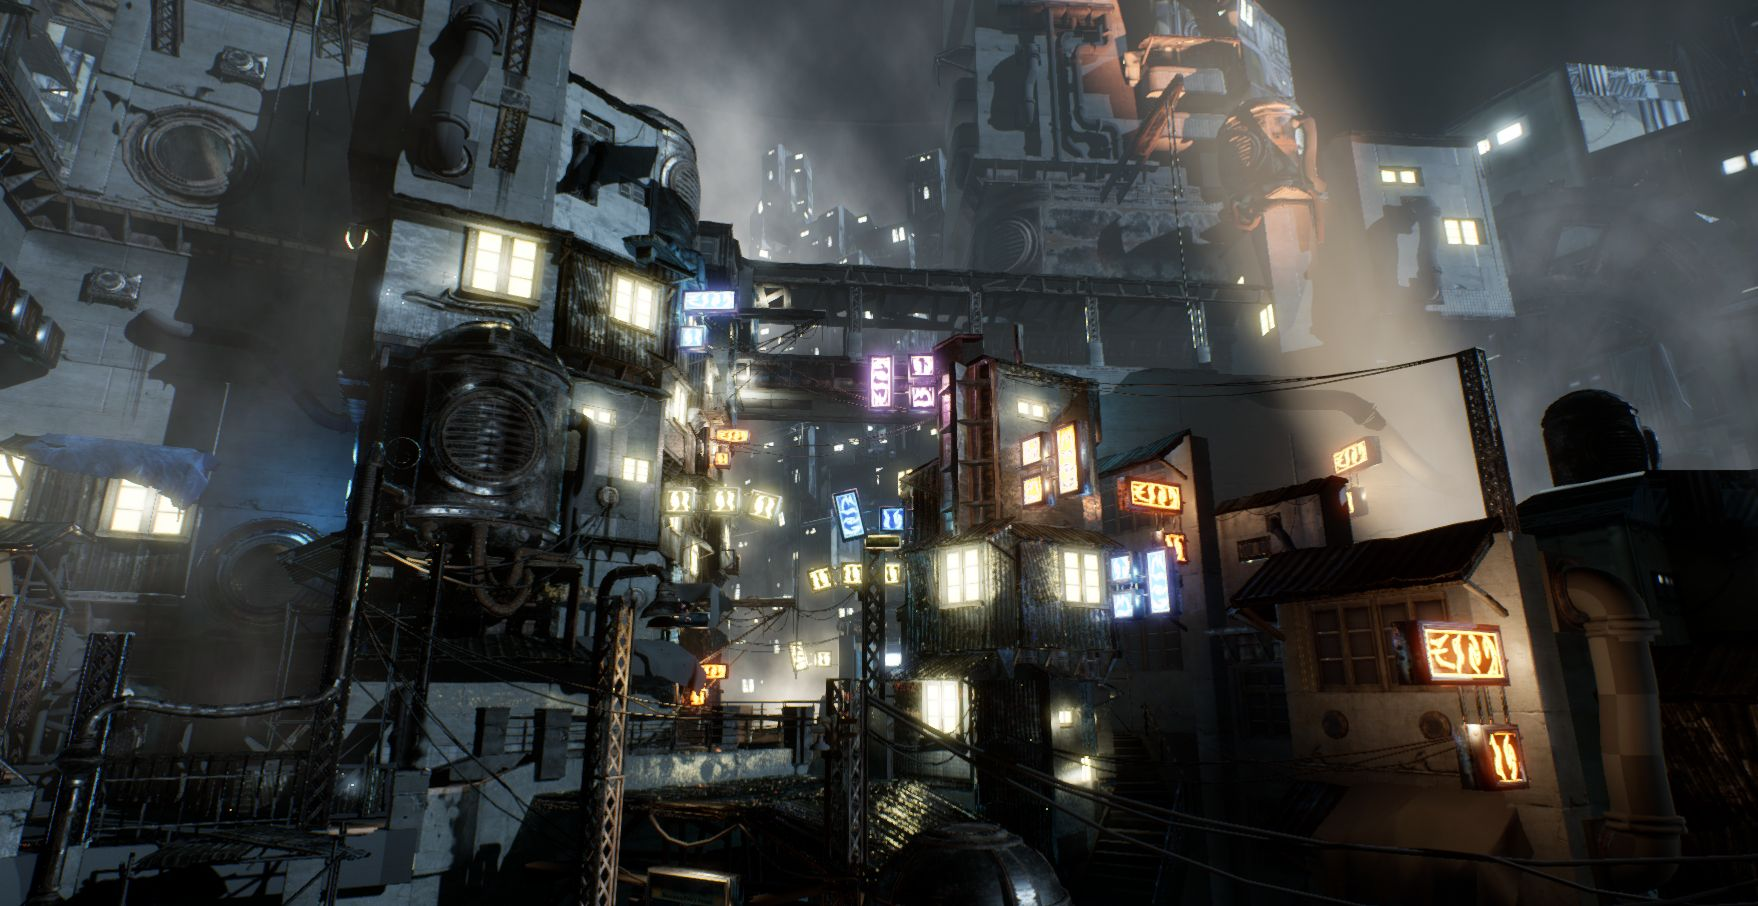
\includegraphics[width=0.95\textwidth]{images/07cha_06_SoulCityUnrealDemo.jpg} 
	\caption{The \emph{Soul: City} map \cite{epic2018soul} using different reusable materials for shading. The scene is highly optimized to run on mobile devices. Image source: \cite{epicimage2018soul}. }
	\label{fig:soulscene}
\end{figure}

\begin{figure}
	\centering\small 
	\begin{tabular}{@{}cc@{}} % mittlerer Abstand = 12mm
		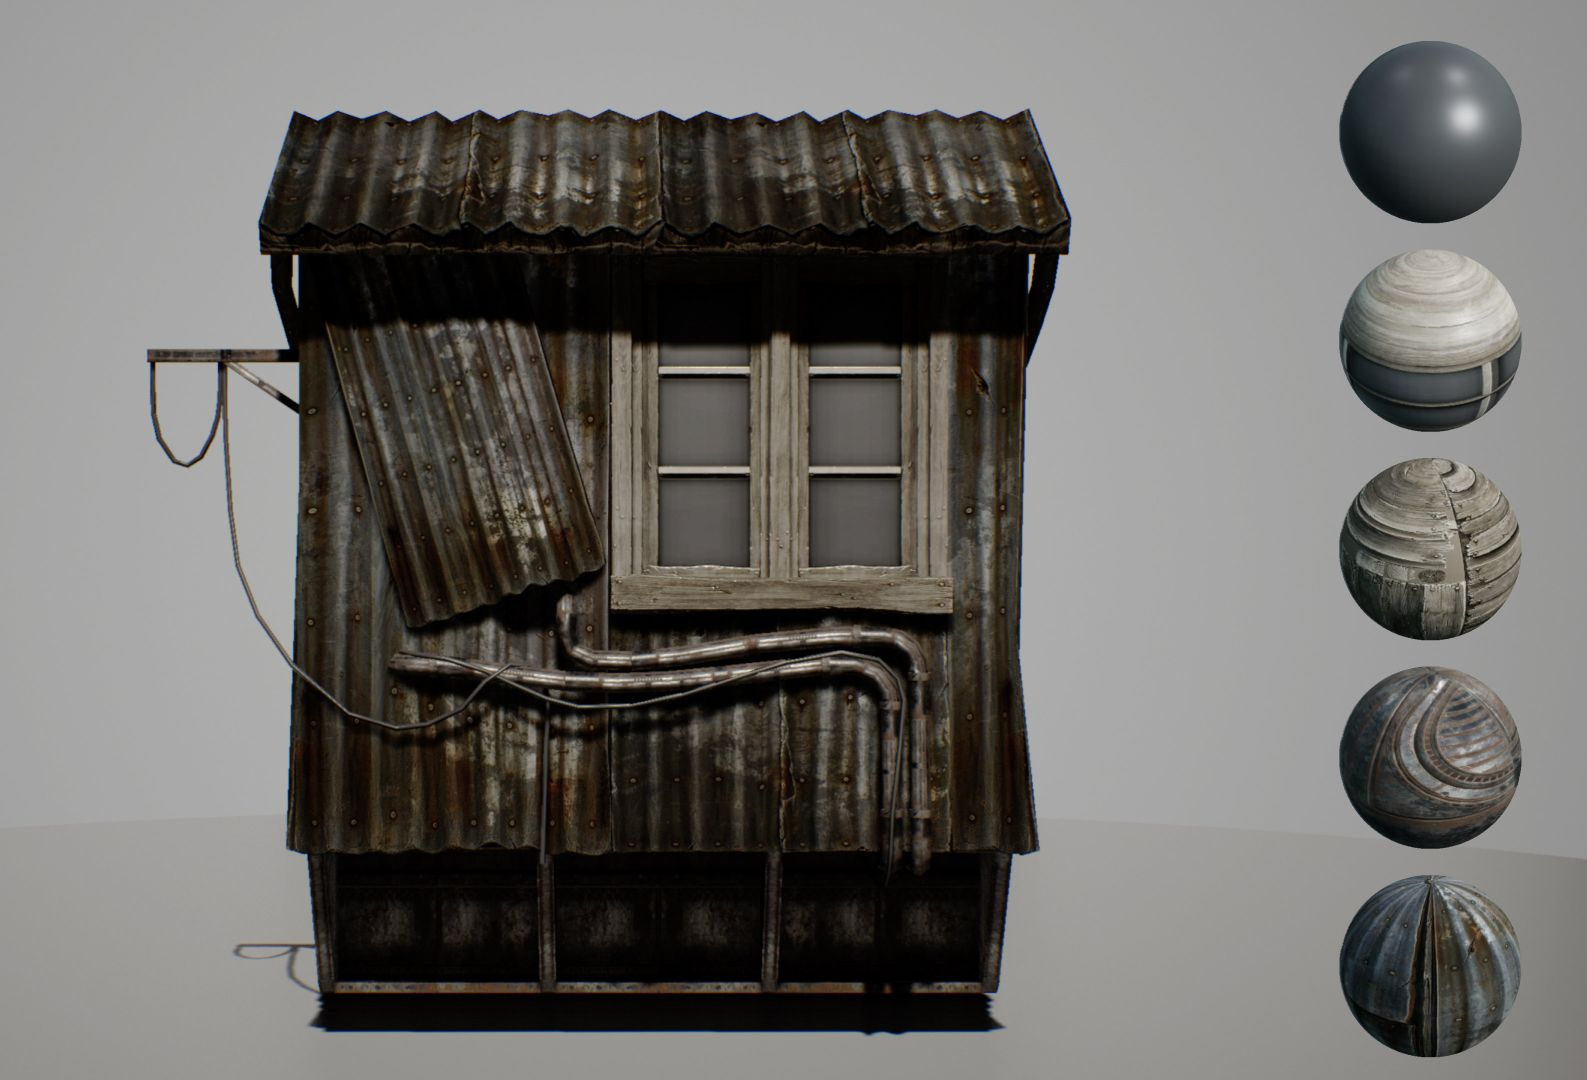
\includegraphics[width=.475\textwidth]{07cha_07_pattern_mutliMat_01.jpg} &
		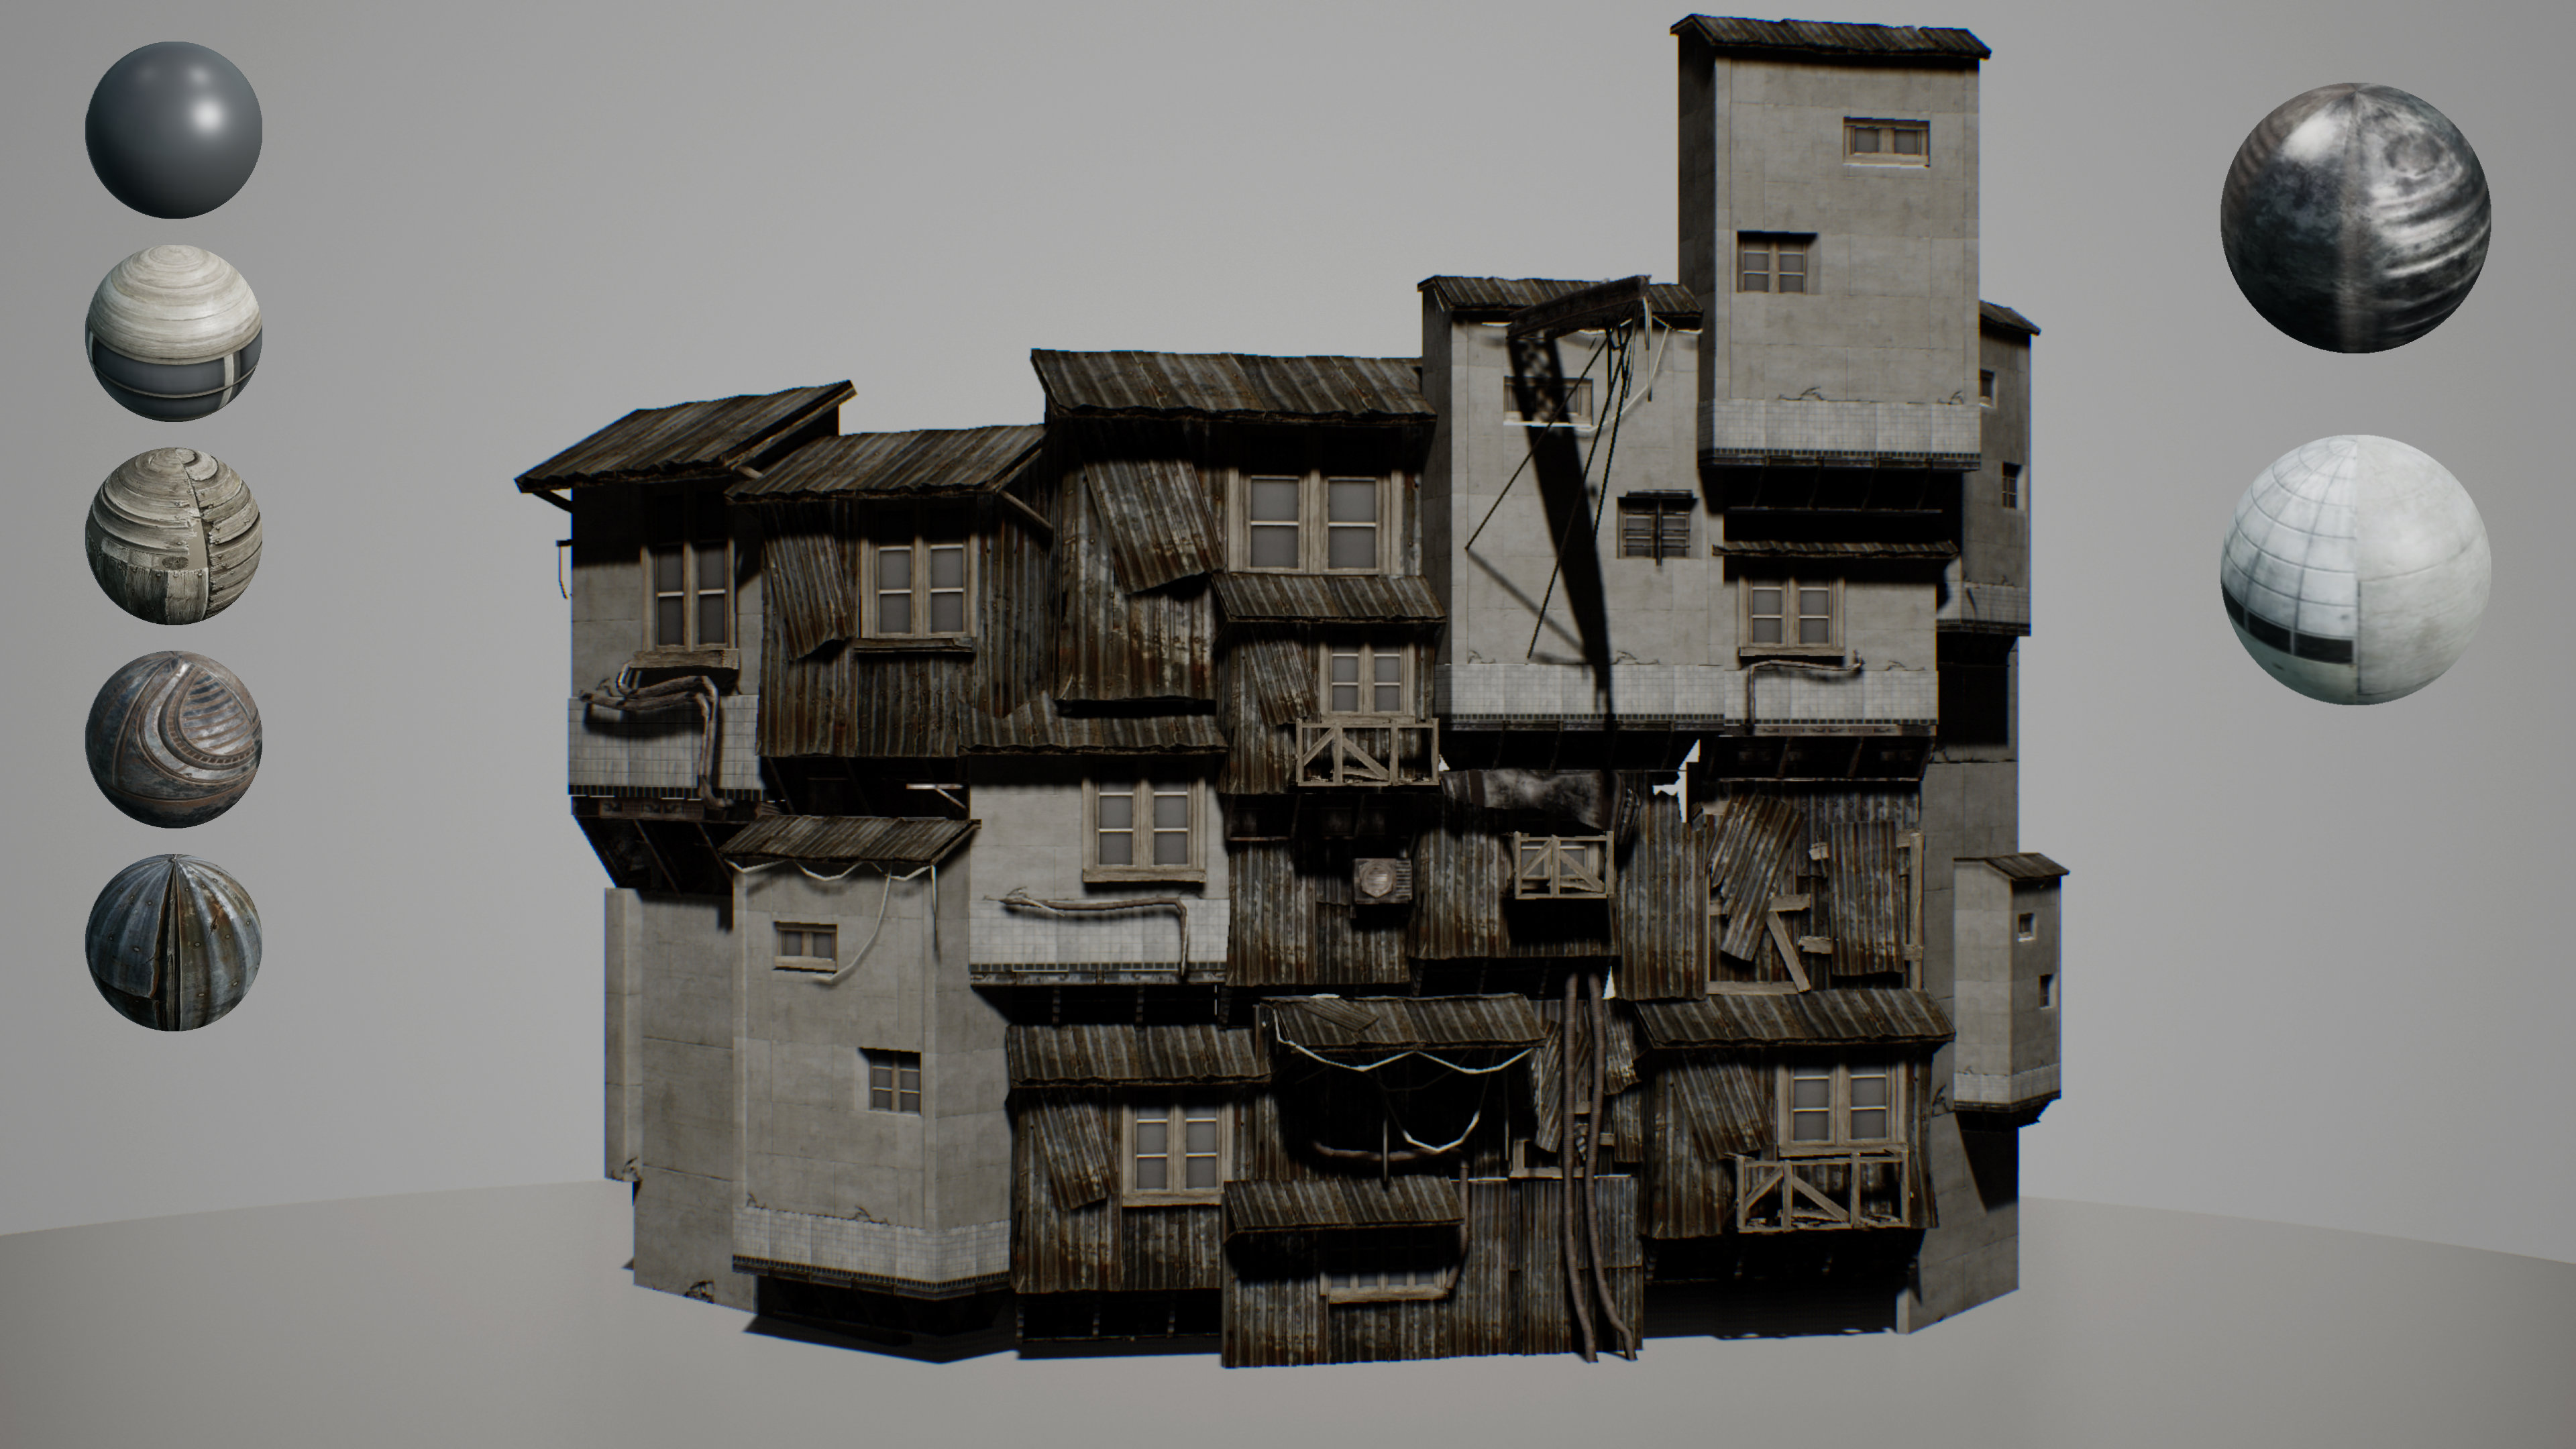
\includegraphics[width=.475\textwidth]{07cha_07_pattern_mutliMat_02.jpg} \\
		(a) & (b)
	\end{tabular}
	\caption{Different assets sharing generic, reusable materials.
		These renderings are made from \emph{Soul: City} assets \cite{epic2018soul}. Figure (a) shows one of those assets. It is textured by using five distinctive mesh independent materials. They are reused across all city assets. Figure (b) shows different assets merged together. The material count increases only slightly. All mesh parts using the same material can now be batched for rendering.  }
	\label{fig:multiMatsSoul}
\end{figure}

%%%%%%%%%%%%%%%%%%%%%%%%%IMPLEMENTATION%%%%%%%%%%%%%%%%%%%%%%%%%%%%%%%%%%%%%%%


\section{\patCatShaderModel}\label{\patCatShaderModel}

After deciding to use pattern layering for your project, the next big questions arise: How to implement and use pattern layering as well as how to structure and organize the shaders and materials. The following categories \emph{\patCatShaderImplementation} and \emph{\patCatWorkflow} will provide patterns to help you making these high level decisions. They will help you to evaluate the benefits and constraints of using pre-existing shaders. What opportunities and dangers arise from creating a custom pattern layering shader or system? Is it better to create a centralized all purpose shader or problem specific custom shaders for my particular project?  

\subsection{\patCatShaderImplementation}\label{\patCatShaderImplementation}

Resources, budgets and requirements differ from project to project. Patterns \emph{\patImplementationBUildtIn} (section \ref{\patImplementationBUildtIn}) and \emph{\patImplementationCustomShader} (section \ref{\patImplementationCustomShader}) propose different approaches to include pattern layering into your workflow. They discuss the benefits and limitations of pre-existing shaders and workflow as well as challenges when creating a custom setup.\,These patterns will help weigh up the two possibilities with regard to effort and benefit. 

\subsubsection{\patImplementationBUildtIn}\label{\patImplementationBUildtIn}
\begin{description}
	\item[\patIntent:]% 
	Use pre-existing pattern layering solutions for your project and purpose. These take care of the complex blending of individual base materials but limit the amount of base materials, the kinds of inputs utilized to generate the base materials and masks as well as the used blending modes. 
	%\item[\patAlsoKnownAs:]% 
	\item[\patMotivation:]% 	
	Consider a project utilizing photogrammetry. The \emph{layeredLit} shader, included in the \emph{HDRenderPipeline} package, provides all the functionality needed. Different sources explain the workflow in detail (e.g., webblogs and articles like this one \cite{unity2017photogrammetryLayered}) and facilitate the adaptation to the personal pipeline. The deadline to deliver the environment assets is in a few weeks. The texturing pipeline is highly texture based and already utilizes the \emph{Substance Painter}. The desired visual quality and texel density cannot be achieved by pre-baked texture, \emph{\patAlternativeBaked} (section \ref{\patAlternativeBaked}). \emph{Allegorithmics} layered material shader for \emph{Unity} and \emph{UE4} provides tools and a predefined pipeline. This is an easy way to incorporate pattern layering into your workflow. Because of its texture based base material and masking workflow, it is easy to use and allows the shipping of the final product in time. 
	\item[\patApplicability:]\hfill
	\begin{itemize}\mynobreakpar
		\item The requirements for the shader are already met by pre-existing shaders (e.g., \emph{Unitys LayeredLit} shader for photogrammetry data).
		\item There is no development budget to create and test custom shaders and pipeline tools.
		\item In comparison to using \emph{custom shaders}, see \emph{\patImplementationCustomShader} (section \ref{\patImplementationCustomShader}), it affords less technical knowledge.  
		\item The project does not require complete control over every single aspect of the rendering process.
		\item  You prefer spending time in creating assets and art to struggling with technical challenges and shaders. 
	\end{itemize} 
	\item[\patImplementation:]% 
	\emph{Unity} ships with the \emph{LayerdLit} and \emph{LayeredLitTessellation} shaders. When using the \emph{HDRenderPipeline}, a new material can easily be created using these shaders. They combine object specific textures with tilable base materials, \emph{\patPatternLayeringHybrid} (section \ref{\patPatternLayeringHybrid}). Other layered material shaders can be downloaded from \emph{Allegorithmic's Substance Share} Website.\footnote{The following website contains layered materials shaders for both \emph{UE4} and \emph{Unity}: \url{https://share.allegorithmic.com/libraries?by_category_type_id=15}.} These shaders are available for both \emph{Unity} and \emph{UE4}. These are  purely pattern based---\emph{\patPatternLayering} (section \ref{\patPatternLayering})---and rely entirely on texture based material inputs (see pattern \emph{\parParametersTextures} in section \ref{\parParametersTextures}). Further information on the \emph{LayeredLit} and \emph{Layered Material} shaders can be found in section \ref{sec:preexistingShaders}. 
	\item[\patExamples:]% 
	Different examples for built-in shaders can be found in section \ref{sec:preexistingShaders}. \emph{Unity's} \emph{Fontainebleau} \cite{fontainebleu2018} demo illustrates the power of the previously explained \emph{LayeredLit} shader. Figure \ref{fig:layeredLitFontainebleau} shows an exterior scene using photogrammetry in combination with a built-it pattern layering shader. The scene was created to represent a real game level. It targets a frame rate of 30fps on a standard PlayStation 4. Using a preexisting solution like this one can save months of development and testing effort. 
	\item[\patConsequences:]\hfill 
		\begin{description}
			\item[\visual:]\hfill
			\begin{itemize}\mynobreakpar
				\item The possibilities are limited by the used shader.
				\item These shaders are normally designed for general purposes as they are made to account for different situations and projects. 
				\item They provide only a limited control over the amount of layers, inputs used for the individual base materials and masks as well as the blending.
				\item Procedural inputs for manipulating masking, base material creation and blending are most likely not implemented into the shader (e.g., vertex color, world space normal and world position) 
			\end{itemize}
			\item[\performance:]\hfill
			\begin{itemize}\mynobreakpar
				\item These shaders are already optimized and hopefully tested on multiple platforms.
				\item They don't provide any control for optimizing performance usage. 
			\end{itemize}
			\item[\pipeline:]\hfill
			\begin{itemize}\mynobreakpar
				\item Built-shaders handle complex blending of the individual parameters between base materials automatically. 
				\item They are already integrated into predefined pipelines. These pipelines can easily adapted to the current project. 
				\item They limit the possibilities layered materials offer dramatically. 
			\end{itemize}
		\end{description}
	\item[\patRelations:]% 
	A Built-in shader is most probably implemented as a \emph{\patWorkflowUberShader} (section \ref{\patWorkflowUberShader}) and does only use texture based inputs for the base material description and masking.  %(see pattern \ref{pat:Texture Inputs} and {\TODO .... TODO .....}) as 
	This kind of shader is designed to fit many different purposes and to be intuitive. %Most artist are used to working with textures.  
\end{description}


\begin{figure}
	\centering
	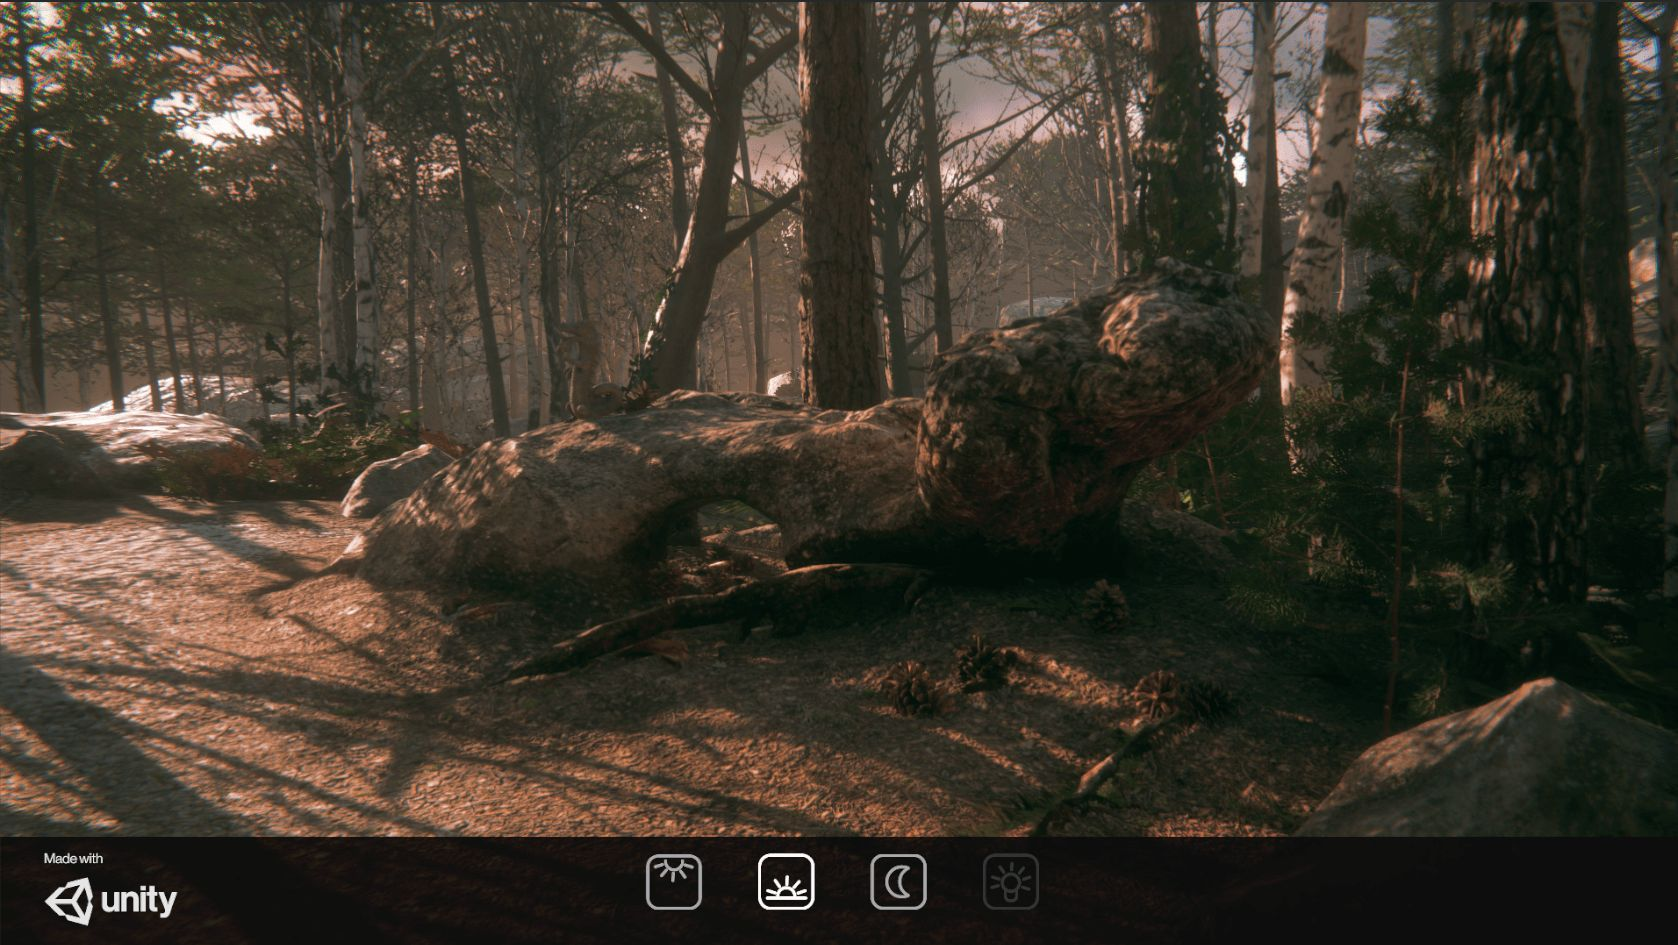
\includegraphics[width=0.7\linewidth]{images/07cha_08_image8.jpg}
	\caption{Fontainebleau \cite{fontainebleu2018}, creating a realistic scene by combing photogrammetry with pattern layering. Image source: \cite{legarde2018photogrammetry}. }
	\label{fig:layeredLitFontainebleau}
\end{figure}
%This example uses the \emph{LayeredLit} shader \cite{legarde2018photogrammetry}. It runs with a constant frame rate of 30 on a standard Playstation 4

\subsubsection{\patImplementationCustomShader}\label{\patImplementationCustomShader}
\begin{description}
	\item[\patIntent:]% 
	Create custom shaders to control every aspect of the material layering process (e.g., material containers, masking containers and blending modules). This provides huge control over accuracy and performance as well as the used number of layers, used masking methods and utilized inputs. However, it comes with the cost of manually optimizing the performance, ensuring the proper blending of individual materials and testing all aspects.  
	%\item[\patAlsoKnownAs]% 
	\item[\patMotivation:]% 
	You are assigned with the task of shading and texturing a huge exterior scene. The scene consists of rocks surrounding a small lake. The moss is supposed to cover the top of the rocks. Areas close to the water should be covered by more moss than areas further away. Instead of creating individual masks for all the objects, you can utilize procedural methods. Using world space normals enables you to easily mask out areas facing to the top. Additional data, like world space position and tileable texture masks, can be used to add further detail. This procedural approach enables rotating the individual assets and all the masks adapt dynamically. Incorporating vertex color into the shader enables controlling the masking further. For instance, blue vertex color adds and red color removes  areas from the mask. Custom shaders provide the flexibility to implement systems like this.
	\item[\patApplicability:]\hfill
	\begin{itemize}\mynobreakpar
		\item Customs Shaders provide full flexibility in the amount and complexity of base materials. 
		\item Using custom shaders is most likely the only possibility to use procedural methods for base material or mask definition within your material (e.g., masks based on world position normal or color tint depending on position). 
		\item The masking between different base materials is not only based on texture masks but also incorporates different parametric inputs and scene data. 
		\item A budget to develop custom layered material shader and additional pipeline tools exists.
		\item There is time to carefully test the layered material shader and its individual parts. 
		\item The complete control over performance usage and optimization is needed and used. 
	\end{itemize}
	\item[\patImplementation:]% 
	\emph{Unity} and \emph{UE4} provide different possibilities for implementing pattern layering. These methods are described in chapter \ref{cha:implementationParametricLayering}. Both engines support the shading languague HLSL/Cg and node based shader graphs. Additionally, \emph{UE4} provides two dedicated systems to create layered materials (see section \ref{sec:matLayV1} and section \ref{sec:matLayV2}).
	\item[\patExamples]% 
	Huge \emph{AAA} video game productions like \cite{witcher2015cdproject, order2015readyatdawns, naugthy2016uncharted, paragon2016epic, gears2016coalition}%
	use custom shading solutions. This provides the developers with the maximum control over visual appearance and performance. \emph{Letzte Worte} uses custom shaders for most of the environment assets. Most of the patterns presented in this catalog were implemented and evaluated within this project.
	\item[\patConsequences:]\hfill 
		\begin{description}
			\item[\visual:]\hfill
			\begin{itemize}\mynobreakpar
				\item Custom Shaders provide the most artistic freedom in terms of what is possible.
				\item A big part of the artistic process takes place while creating the shader. 
				\item It represents a highly technical approach in the handling texturing. 
				\item Shaders can be utilized to solve blending and material creation fully or partially. 
				\item This approach requires a ot of technical knowledge.  
			\end{itemize}
			\item[\performance:]\hfill
			\begin{itemize}\mynobreakpar
				\item Custom shaders provide the full control over resource usage and performance. 
				\item Achieving good performance requires a lot of testing and optimization.
				\item Custom shaders are error prone for bad performance. 
			\end{itemize}
			\item[\pipeline:]\hfill
			\begin{itemize}\mynobreakpar
				\item Iterating on different base materials and masks is fast. 
				\item Iterations on the implemented shader are difficult and slow. 
				\item Creating stable shaders is time consuming and requires a lot of experience. 
				\item A lot of testing is needed, especially if the shader offers many different switches and states. 
				\item Shaders need to be tested on all applications the final product appears on. Consoles and mobile devices may not support certain features the shader uses. 
				\item You have the power and responsability to take full controll over features, performance and usability. 
			\end{itemize}
		\end{description}
	\item[\patRelations:]% 
	Patterns \emph{\patWorkflowUberShader} (section \ref{\patWorkflowUberShader}), \emph{\patWorkflowIndividualShader} (section \ref{\patWorkflowIndividualShader}), \emph{\patWorkflowContentDrivenShader} (section \ref{\patWorkflowContentDrivenShader}) show different ways to include custom shaders into the project pipeline. Patterns in the categories \emph{\patCatMaterialContainer}, \emph{\patCatMaskingContainer} and \emph{\patCatBlendingModule} provide further information on how to design and implement the individual components.
\end{description}



%%%%%%%%%%%%%%%%%%%%%%%%%WORKFLOW%%%%%%%%%%%%%%%%%%%%%%%%%%%%%%%%%%%%%%%

\subsection{\patCatWorkflow}\label{\patCatWorkflow}

Organizing and structuring your assets are important tasks. The following patterns discuss different methods on how to  choose and design shaders and systems to fit into what your workflow needs. \emph{\patWorkflowUberShader} (section \ref{\patWorkflowUberShader}) illustrates a workflow with few centralized multi-purpose shaders that cover most of the use cases within your project. Changes, fixes and optimizations within the shader are global and apply to all materials using this shader. Every additional feature increases the complexity of the shader. \emph{\patWorkflowIndividualShader} (section \ref{\patWorkflowIndividualShader}) demonstrates the opposite approach to creating case specific shaders. Individual shaders do only incorporate the functionality for a unique purpose and are therefore more lightweight. 

\subsubsection{\patWorkflowUberShader}\label{\patWorkflowUberShader}
\begin{description}
	\item[\patIntent:]% 
	Create shaders to fit all or most of the needs for a specific kind of objects, like all environment assets or characters. This way, changes are propagated to all materials.
	\item[\patAlsoKnownAs:]% 
	\emph{Master Material}	
	\item[\patMotivation:]% 	
	Consider a project with many different interior scenes. The modular, wall and floor assets are supposed to use pattern layering. The features required for the shader are clear: UV or world position based texture mapping, the base materials and masks are texture based. Additionally, it is possible to add a random tint. A technical artist designs the shader. The shader is tested by the artists creating a test scene and simultaneously optimized to work properly on all devices.
	\item[\patApplicability:]\hfill
	\begin{itemize}\mynobreakpar
		\item When working with built-in shaders (\emph{\patImplementationBUildtIn} in section \ref{\patImplementationBUildtIn}), you are most likely using an \emph{Uber Shader} as they are generally designed to fit general purposes.
		\item The shader is supposed to work for a wide variety of situations and probably for different projects. 
		\item A multi-purpose shader is created by a developer or technical artist, tested extensively on all devices the project is developed for. The shader is handed over to artists and not supposed to change dramatically.
		\item The feature requirements for the shader are limited. Most of the materials need similar parameters.  
	\end{itemize}
	\item[\patImplementation:]% 
	The implementation of an uber shader is not different from implementing a individual shader, see \emph{\patWorkflowIndividualShader} (section \ref{\patWorkflowIndividualShader}). The difference is mainly in the design, i.e., which parameters are exposed to the individual materials. Uber shaders and individual shaders can be used to complement one another in the same project.
	\item[\patExamples:]% 
	Many of the environment assets within \emph{Letzte Worte} use the same uber shader. Especially, the first location does almost exclusively use uber shaders to define all materials. Figure \ref{fig:leaFurniture} shows one of those assets. They were initially used to unify the shading workflow and make it easy to change individual materials. In the later stage of the production, I created more individual shaders to reduce the texture count and to better incorporate procedural methods into the shader creation.
	\item[\patConsequences:]%
		\begin{description}
			\item[\visual:]\hfill
				\begin{itemize}\mynobreakpar
					\item The visual posibilites are provided by the uber shader. Every feature needs to be implemented in this shader. The visual variety and style is therefore highly influenced by it.
				\end{itemize}
			\item[\performance:]\hfill
				\begin{itemize}\mynobreakpar
					\item Extensive testing is necessary to ensure an efficient performance. 
					\item It shares all performance limitations of pattern layering (see \emph{\patPatternLayering} in section \ref{\patPatternLayering}).
				\end{itemize}
			\item[\pipeline:]\hfill
				\begin{itemize}\mynobreakpar
					\item Changes and modifications are propagated across all materials using this uber shader, i.e., fixes as well as errors are applied to all materials instantly. 
					\item The shader can get really complex to account for all cases needed. 
					\item Maintaining and sharing this shader with others can get complicated due to its complexity.
					\item The shader may offer a lot of flexibility for the artist in enabling and disabling shader features. 
					\item Extensive testing is important because the shader has to account for many different scenarios and later changes will influences all materials using this shader.
				\end{itemize} 
		\end{description}
	\item[\patRelations:]%
	Built-in shaders, \emph{\patImplementationBUildtIn} (section \ref{\patImplementationBUildtIn}), are generally implemented as uber Shaders, due to their intent on fitting general purposes. Further, they generally use a full material properties description, see \emph{\patComplexityFulMaterial} (section \ref{\patComplexityFulMaterial}). 
\end{description}

\begin{figure}
	\centering
	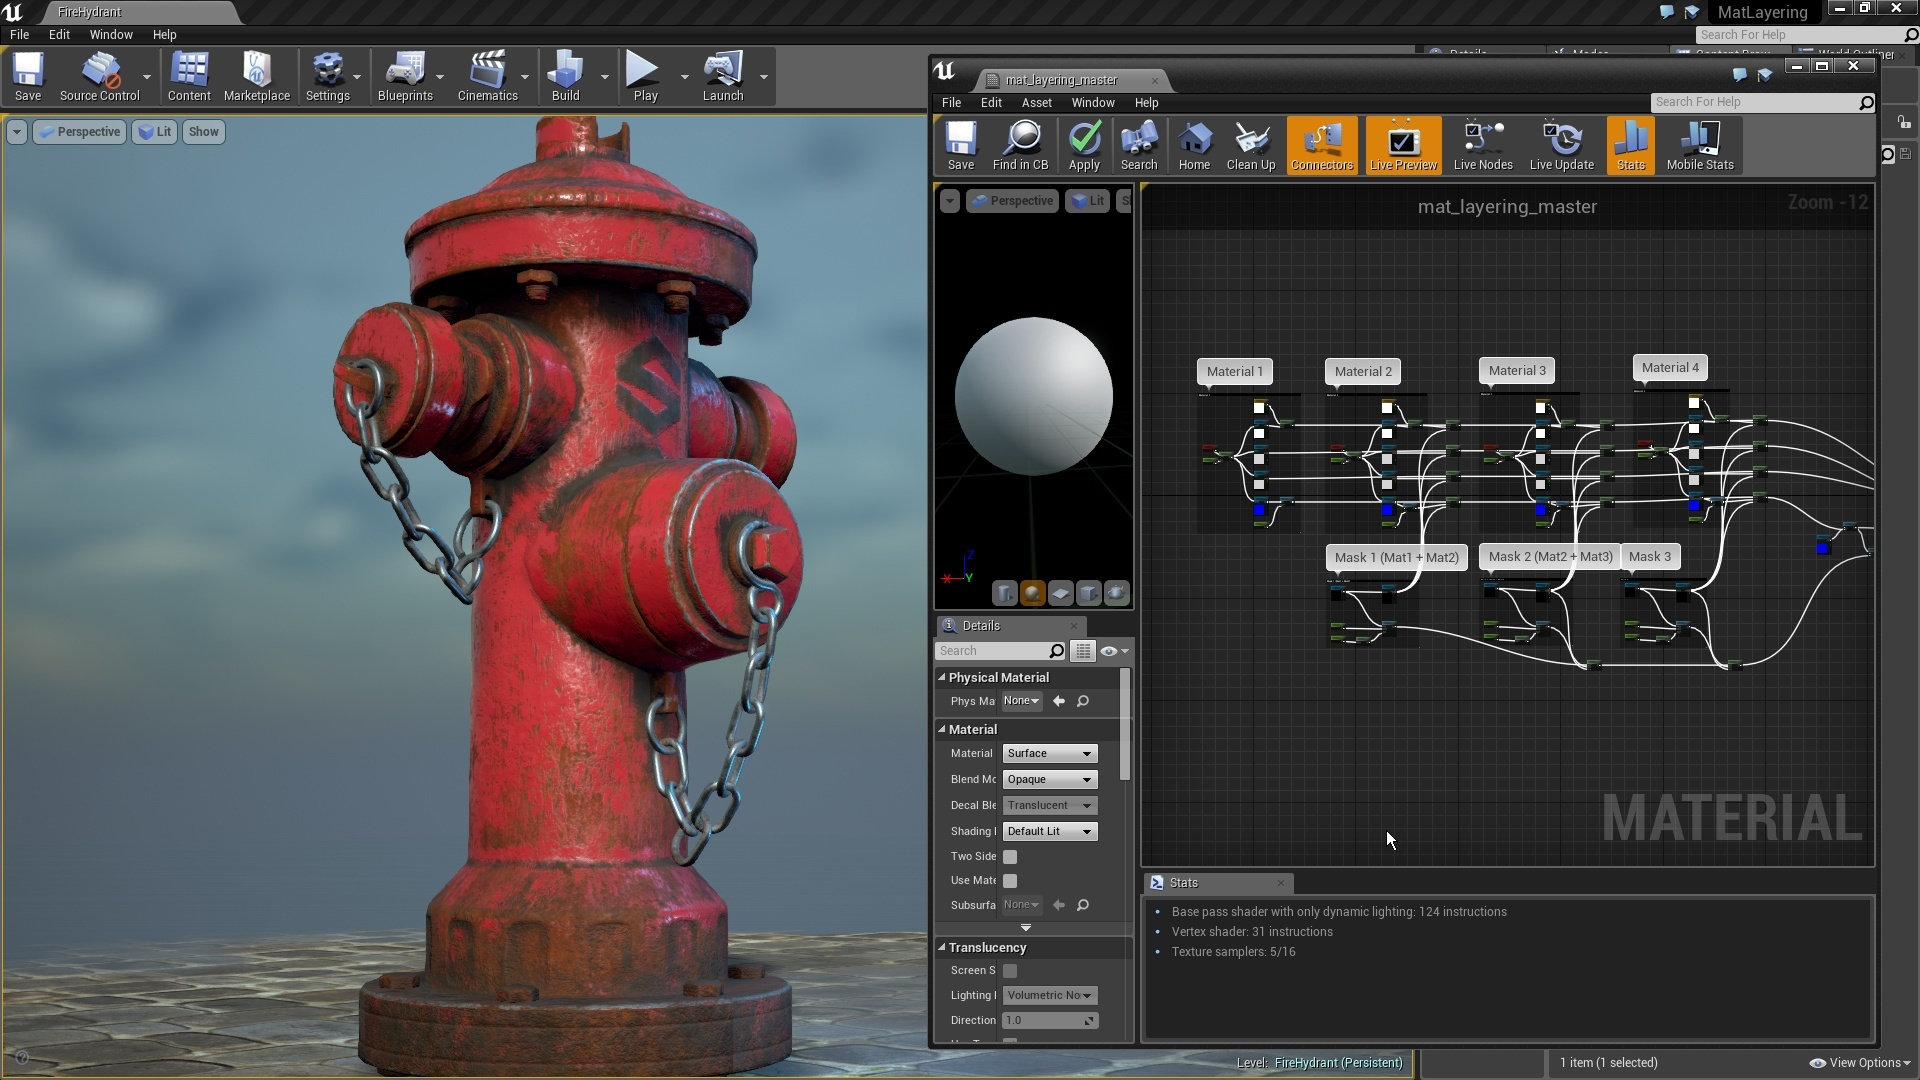
\includegraphics[width=0.7\linewidth]{images/07cha_09_ue4_shader_render.jpg}
	\caption{The material layering shader provided by \emph{Allegorithmic} for \emph{UE4}. Image source: \cite{allegorithmic2016matlay}.}
	\label{fig:uberue4shaderrender}
\end{figure}

\begin{figure}
	\centering
	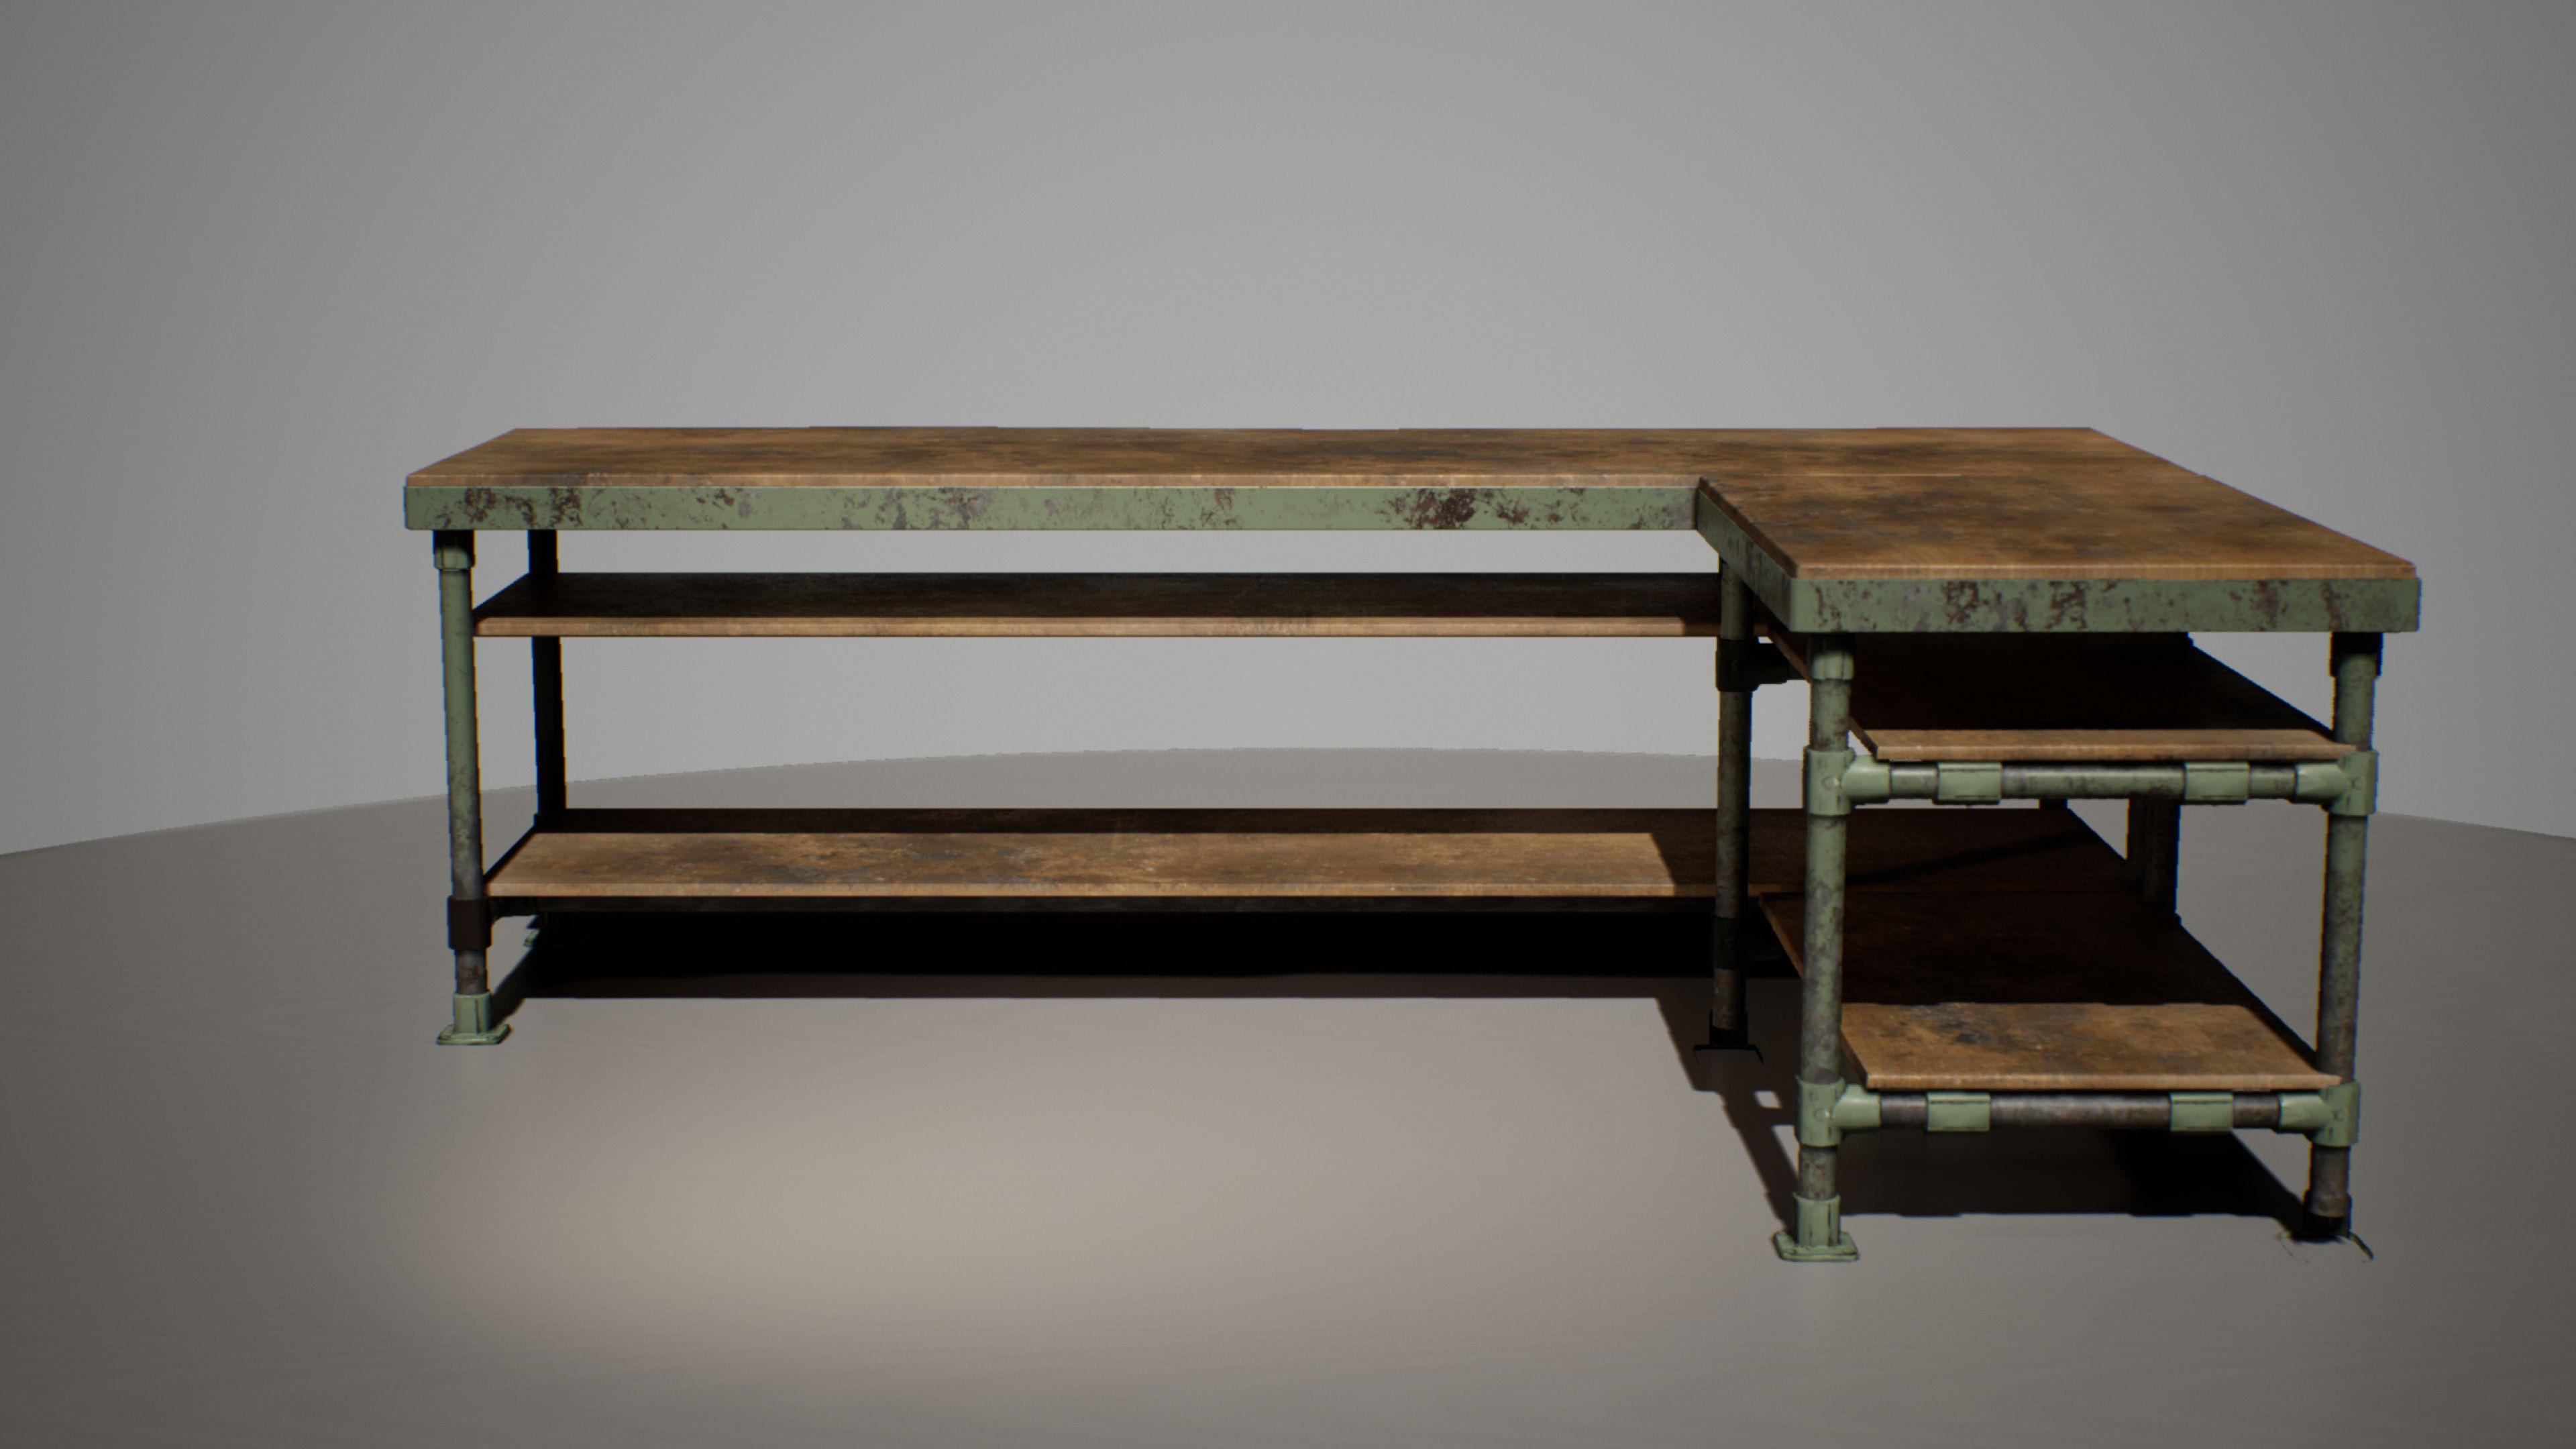
\includegraphics[width=0.7\linewidth]{images/07cha_10_pattern_LeaAssets_Furniture.jpg}
	\caption{ An assets from \emph{Letzte Worte} using a standardized \emph{Uber Shader}. }
	\label{fig:leaFurniture}
\end{figure}
%This allows to create one centralized shader for multiple purposes.

\subsubsection{\patWorkflowIndividualShader}\label{\patWorkflowIndividualShader}
\begin{description}
	\item[\patIntent:]% 
	Create individual shaders to fit the requirements of unique or problem specific needs. These are single purpose shaders and not intended to be used in many different ways. 
	%\item[\patAlsoKnownAs:]% 
	\item[\patMotivation:]% 
	Consider a hero object within your scene. The player triggers a game play element by touching the object and so cause the object to change the material state. The object material transitions from a clean golden metal into an old, aged version covered with dirt and dust. This shading feature is unique to this particular case. In an other example, a few objects within your scene are made of fur. The shading requirements are really similar for all of them. You create a shader with custom fresnel, parallax occlusion mapping and other features specifically designed for this fur shading.
	\item[\patApplicability:]\hfill
	\begin{itemize}\mynobreakpar
		\item The shader does only need to cover one specific use case. It is unique in its requirements. Incorporating this functionality into a uber shader would only increase the complexity of the shader.
		\item It enables a more artistically driven shader creation. For instance, specific shaders can be created to fit the artistic goal of an object.
	\end{itemize}
	\item[\patImplementation:]% 
	Individual shaders are implemented either as \emph{\patPatternLayering} (section \ref{\patPatternLayering}) or \emph{\patPatternLayeringHybrid} (section \ref{\patPatternLayeringHybrid}) and use most likely \emph{\patImplementationCustomShader} (section \ref{\patImplementationCustomShader})
	\item[\patExamples:]% 
	\emph{Letzte Worte} uses individual shaders for specific use cases. Figure \ref{fig:leaRoomCarpet} shows two of them. The carpet uses a specific shading feature and therefore uses a special shader specifically designed to fit these requirements. The laptop is a gameplay element the player can interact with. This individual shader provides features like switching the screen on or off and changing the desktop of the screen. 
	\item[\patConsequences:]\hfill 
		\begin{description}
			\item[\visual:]\hfill
			\begin{itemize}\mynobreakpar
				\item An individual shaders offers lot of artistic freedom. The shader does only need to fit the demands of few use cases. 
				\item It is much less important to create a user friendly and predictable shader than it is for an uber shader. Only parameters for this use cases need to be exposed, and most likely only a few people will ever work with this shader. 
				\item The shader does not need to fit into the design of an uber shader and is therefore more flexible. 
			\end{itemize}
			\item[\performance:]\hfill
			\begin{itemize}\mynobreakpar
				\item These shaders share all performance limitations of other pattern layering shaders. Testing is essential. 
				\item As they are used only a few times within a project, performance is generally less important than for an uber shader that is used all over. 
			\end{itemize}
			\item[\pipeline:]\hfill 
			\begin{itemize}\mynobreakpar
				\item Changes within the shader are only applied to the individual shader and the few materials using it.  
				\item The shaders are generally less complex than uber shaders as they do not need to cover for all cases. 
				\item The shader development is more artist driven.
				\item Aspects like performance and usability are not as important as for uber shaders.
			\end{itemize}
		\end{description}
	\item[\patRelations:]%
	The only difference to an uber shader, \emph{\patWorkflowUberShader} (section \ref{\patWorkflowUberShader}), is the different complexity and that their usage is limited to only a few use cases. 
\end{description}


\begin{figure}
	\centering
	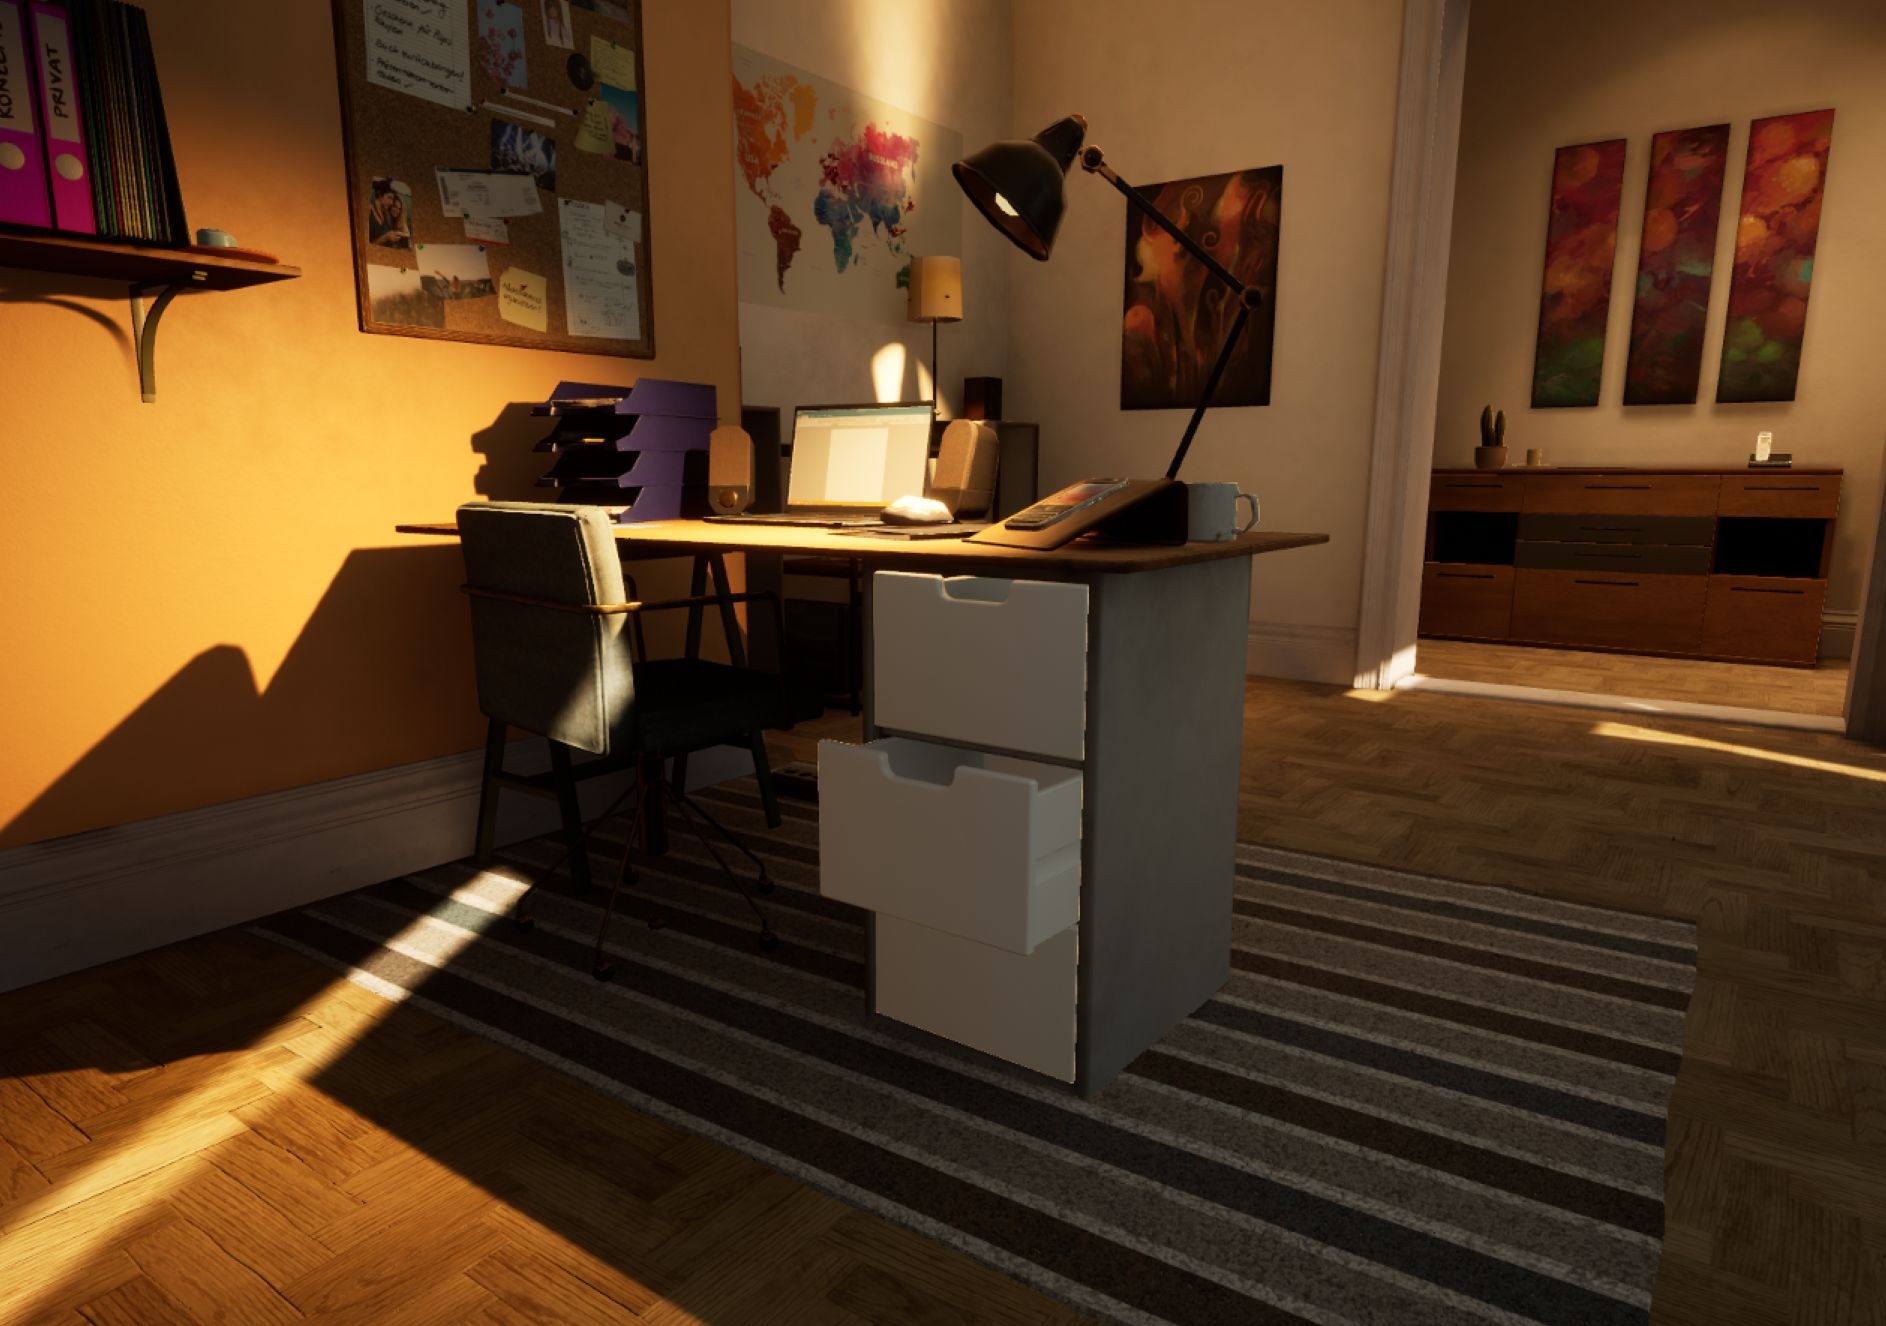
\includegraphics[width=0.7\linewidth]{images/07cha_11_leaRoomCarpet.jpg}
	\caption{Using individual shaders for unique and specific requirements.
		Both the carpet and the laptop use individual shaders as they have specific shader requirements: the carpet uses parallax occlusion mapping for the hair while the laptop material changes states depending on the player interaction (e.g., switching on by opening the laptop).}
	\label{fig:leaRoomCarpet}
\end{figure}

\subsubsection{\patWorkflowContentDrivenShader}\label{\patWorkflowContentDrivenShader}
\begin{description}
	\item[\patIntent:]%
	Use a tool to create automated custom shaders from user given material layers, masks and parameters. The shader is generated automatically based on the inputs, instead of the desired inputs being specified by the shader. This turns the regular workflow---i.e., \emph{\patWorkflowIndividualShader} (section \ref{\patWorkflowIndividualShader}) and \emph{\patWorkflowUberShader} (section \ref{\patWorkflowUberShader})---around.  
	\item[\patAlsoKnownAs:]% 
	\emph{Material Masking System (MMS)},\emph{Material Layers} in \emph{UE4}
	%\item[\patMotivation:]% 
	\item[\patApplicability:]\hfill 
	\begin{itemize}\mynobreakpar
		\item Writing your own tool will not be an option for most cases. Content generated shaders requires highly sophisticated tools. A huge amount of research, development and testing runs into creating such a tool. 
		\item An appropriate tool exists that works with the given real-time engine. The tool is stable, has been tested and covers the needs for the given project. 
		\item A shared, art directed material library does already exists or is planned to be built. 
		\item A huge variety is needed for combining different base materials, masks and blending modes.
	\end{itemize}
	\item[\patImplementation:]% 
	Developing a custom tool is complicated as it has to create shader code automatically from arbitrary material, masking and blending inputs. Additionally, the inputs cannot simply be linearly interpolated  but need to be blended differently depending on data types, parameters and shading algorithms (see section \ref{sec:blendindIssuesLayering} for further details). To the best of my knowledge, \emph{Unity} does not provide any system for this. \emph{UE4} has just recently implemented a corresponding system with their \emph{Material Layers} (see section \ref{sec:matLayV2} for more details). 	
	\item[\patExamples:]% 
	\emph{Gears of War 4} \cite{gears2016coalition} uses a corresponding system for their material pipeline \cite{colin2017GearsOfWar}. See figure \ref{fig:clinton-crumpler-highresscreenshot00024-min}. Another tools is provided by \emph{UE4} as shown in figure \ref{fig:engine19}. 
	\item[\patConsequences:]\hfill 
		\begin{description}
			\item[\visual:]\hfill
			\begin{itemize}\mynobreakpar
				\item The  artistic freedom of contend generated shaders is dependent on the system used. Generally, they allow to specify an arbitrary number of base materials with utilizing different masking methods and blending modes in a user friendly way. Additionally the system automates complicated technical processes of properly blending. 
				\item Individual shading features can be used for different assets. 
			\end{itemize}
			\item[\performance:]\hfill
			\begin{itemize}\mynobreakpar
				\item Ideally the content generated shader does a lot of performance optimization automatically. 
				\item The tool creates input driven individual shaders. Please refer to \emph{\patWorkflowIndividualShader} (section \ref{\patWorkflowIndividualShader}) for further details.   
			\end{itemize}
			\item[\pipeline:]\hfill
			\begin{itemize}\mynobreakpar
				\item The tool provides an easy and fast way to combine and replace material layers. 
				\item Material layers can be replaced by materials using a completely different structure. 
				\item The system provides a modular way to define masking between individual layers.
				\item It is user friendly as the individual components are completely independent and can contain arbitrary data and computation. 
			\end{itemize}
		\end{description}
	\item[\patRelations:]% 
	\emph{\patWorkflowContentDrivenShader} is a system to create \emph{\patWorkflowIndividualShader s} (section \ref{\patWorkflowIndividualShader}) based on the base material inputs, utilized masking method and blending mode.
\end{description}


\begin{figure}
	\centering
	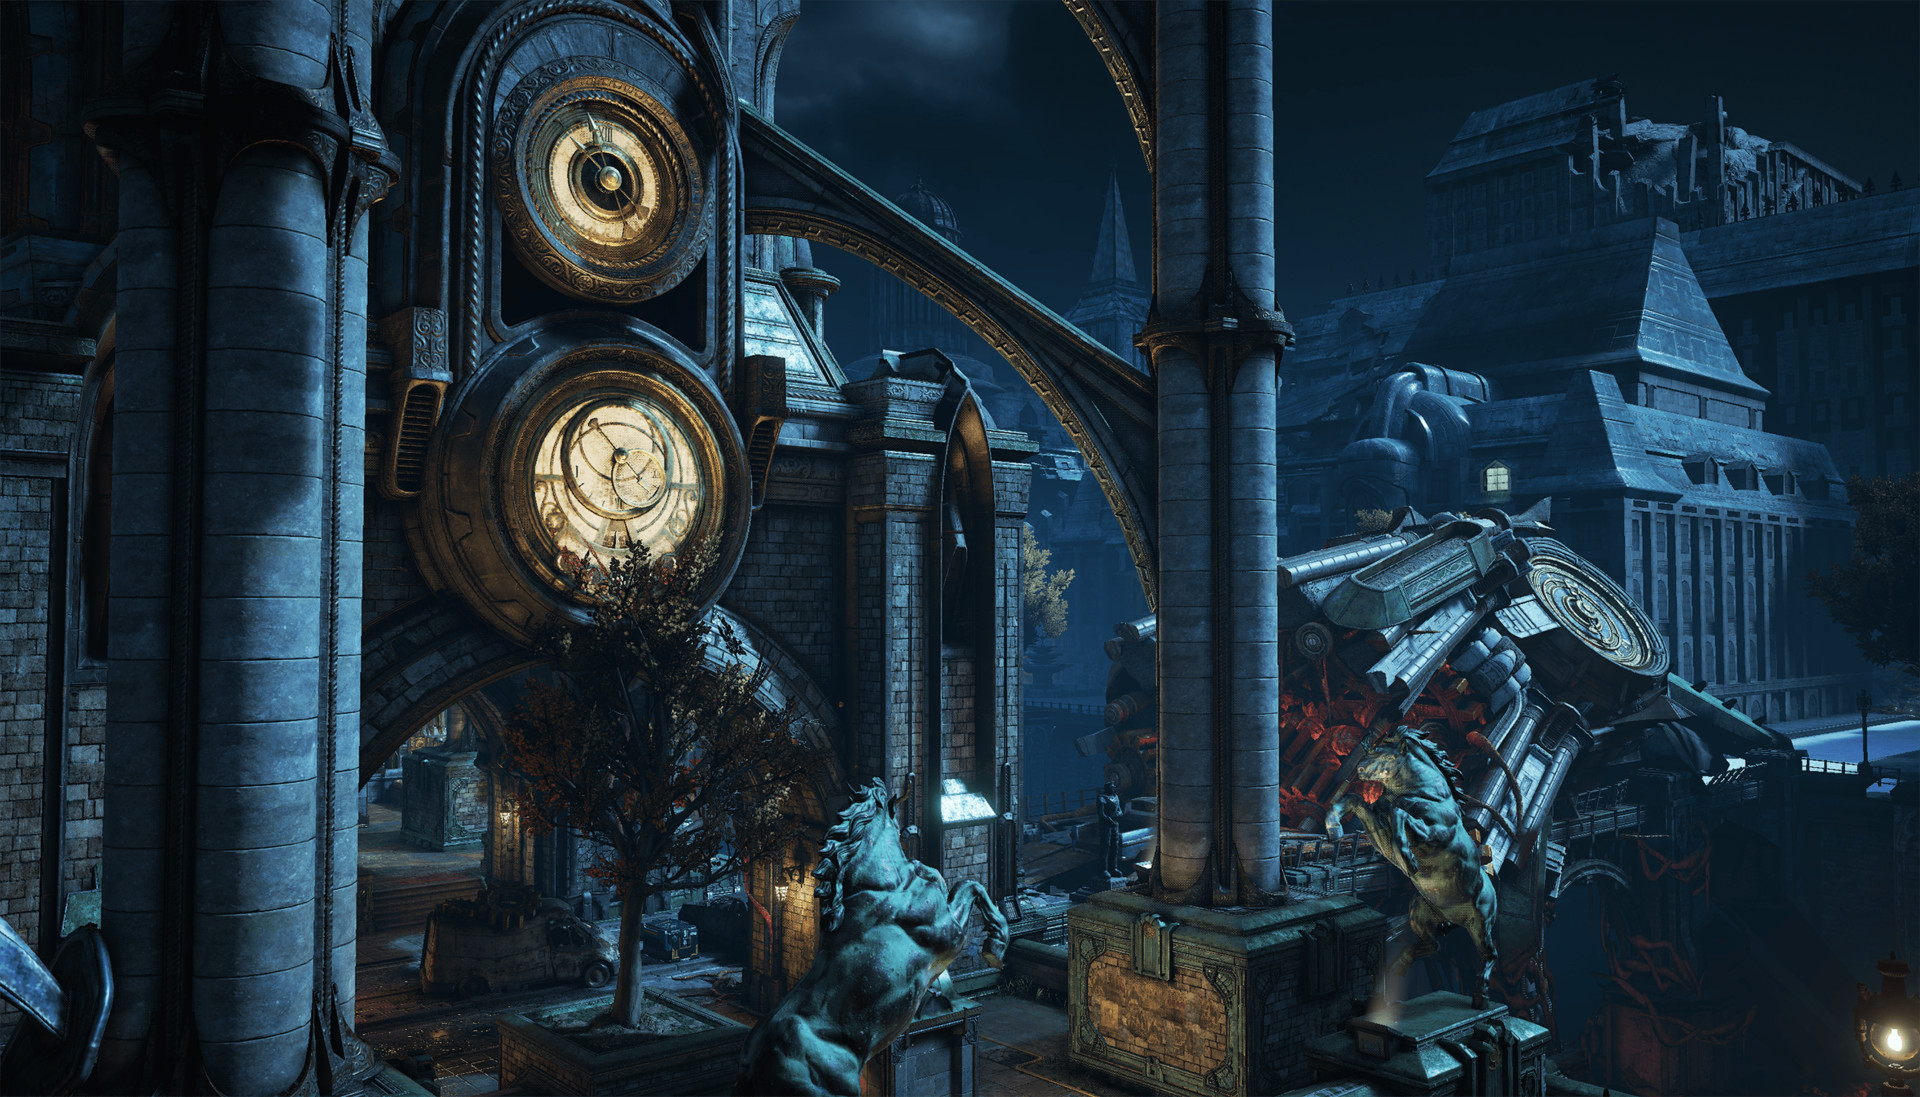
\includegraphics[width=0.7\linewidth]{images/07cha_12_clinton-crumpler-highresscreenshot00024-min.jpg}
	\caption{\NEW
		A scene from \emph{Gears of War 4}. It was created by using their custom material layering tool, the \emph{Material Masking System}. Image source: \cite{crumpler2016Gears}. }
	\label{fig:clinton-crumpler-highresscreenshot00024-min}
\end{figure}

\begin{figure}
	\centering
	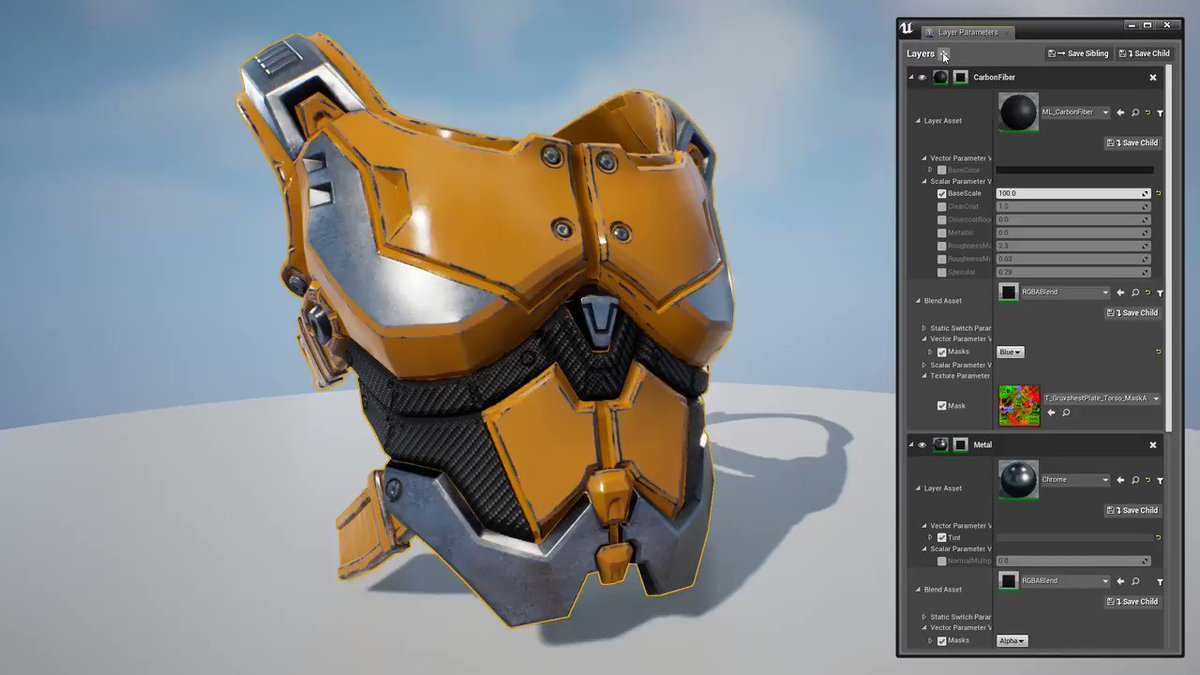
\includegraphics[width=0.7\linewidth]{images/07cha_13_TSUUuOWr5KWbCxN-.jpg}
	\caption{\NEW
		The \emph{Material Layer} system by \emph{UE4}. Image source: \cite{wilson2018ue}.}
	\label{fig:engine19}
\end{figure}


%%%%%%%%%%%%%%%%%%%%%%%%%MATERIAL CONTAINER GRANULARITY%%%%%%%%%%%%%%%%%%%%%%%%%%%%%%%%%%%%%%%

\section{\patCatMaterialContainer}\label{\patCatMaterialContainer}

The following categories correspond to the material layering model defined in chapter \ref{cha:partsOfLayeredShader}. These components are: material container, masking container and blending module. Each category will contain patterns on how to plan and design these components. This first section focuses on the material containers. Core elements of every layered material shader or system are the individual base materials. These base materials are described in the material containers. They use different inputs, can do further computation within the module and output a material layer. These material layers define the surface type and appearance of the final object. The following sections deal with different methods of how to organize and split a surface into individual base materials. They provide patterns on how to define the complexity of individual material containers. Finally, they offer patterns on how and why to use distinctive inputs from within the material container to compute the final material layer. 

\subsection{\patCatGranularity}\label{\patCatGranularity}

As mentioned before, patterns \emph{\patGranularityBase} (section \ref{\patGranularityBase}) and \emph{\patGranularityVariation} (section \ref{\patGranularityVariation}) describe different philosophies on how to split a surface into individual base materials.  \emph{\patGranularityBase} proposes to split a surface by distinctive generic surface types (e.g., metal, rubber, wood, painted wood). Most of the complexity is created by blending those simpler base materials together. Pattern \emph{\patGranularityVariation} describes a method of using more complex base materials containing different surface types and creating different variations of them. This enables the creation of more complex surfaces with fewer base materials but also decreases the use cases for individual base materials.  

\subsubsection{\patGranularityBase}\label{\patGranularityBase}
\begin{description}
	\item[\patIntent:]% 
	Use individual generic base materials to emulate different surfaces and their properties, such as wood, painted wood, steel, rubber etc.  The individual base materials should be generic enough to be reused across many different objects.
	%\item[\patAlsoKnownAs:]% 
	\item[\patMotivation:]% 
	You define a base material library within your project. Recurring base materials like different kinds of wood, metal and fabric get stored in it. Whenever you need a new material, you can add it to the library. The library grows over time. You can texture a new asset by reusing all these generic materials you have already created.
	\item[\patApplicability:]\hfill 
	\begin{itemize}\mynobreakpar
		\item Base materials are used to describe different surface types (e.g., wood, oak wood, painted wood).
		\item The base materials are limited in their complexity. They represent one specific surface type (such as rubber). 
	\end{itemize}
	\item[\patImplementation:]% 
	If you use \emph{\patGranularityBase} or \emph{\patGranularityVariation} is implementation independent. It is a primary a decision of workflow and how to split a surface into base materials. These are rather workflow decisions that simply define how to handle individual layers.
	\item[\patExamples:]% 
	\emph{Letzte Worte} has an exterior scene. See figure \ref{fig:granularityBase}. A path leads from the starting point to the top of the mountain. The environment is textured by reusing the same base materials. These base materials are mainly: rock, moss, ground and forest floor. Each base material represents a different surface type. They are generic enough to be used across different objects. 
	\item[\patConsequences:]%
	\begin{description}
		\item[\visual:]\hfill
			\begin{itemize}
				\item It is easy to change and reuse base materials as they represent surface types.  
				\item The number of different surface types is limited by the shader. Using many base materials increases performance costs and is therefore limited to a few. This decreases surface variety. 
				\item Visual quality and diversity is highly controlled by blending, not necessarily by the base materials.
				\item The blending quality is highly dependent on masking resolution. 
			\end{itemize}
		\item[\performance:]\hfill
			\begin{itemize}
				\item Using a high amount of base materials increases performance costs. 
			\end{itemize}
		\item[\pipeline:]\hfill
			\begin{itemize}
				\item The base materials themselves can be really simple.  
				\item Creating different variations of the shading is simple and fast. You can simply swap two base materials.
				%\item The workflow  highly intuitive. 
			\end{itemize} 
	\end{description}
	\item[\patRelations:]%
	This pattern presents, additionally to \emph{\patGranularityVariation} (section \ref{\patGranularityVariation}), a proposal for how to split your surface into different base materials. 
\end{description}



\begin{figure}
	\centering\small 
	\begin{tabular}{@{}ccc@{}} % mittlerer Abstand = 12mm
		\multicolumn{3}{c}{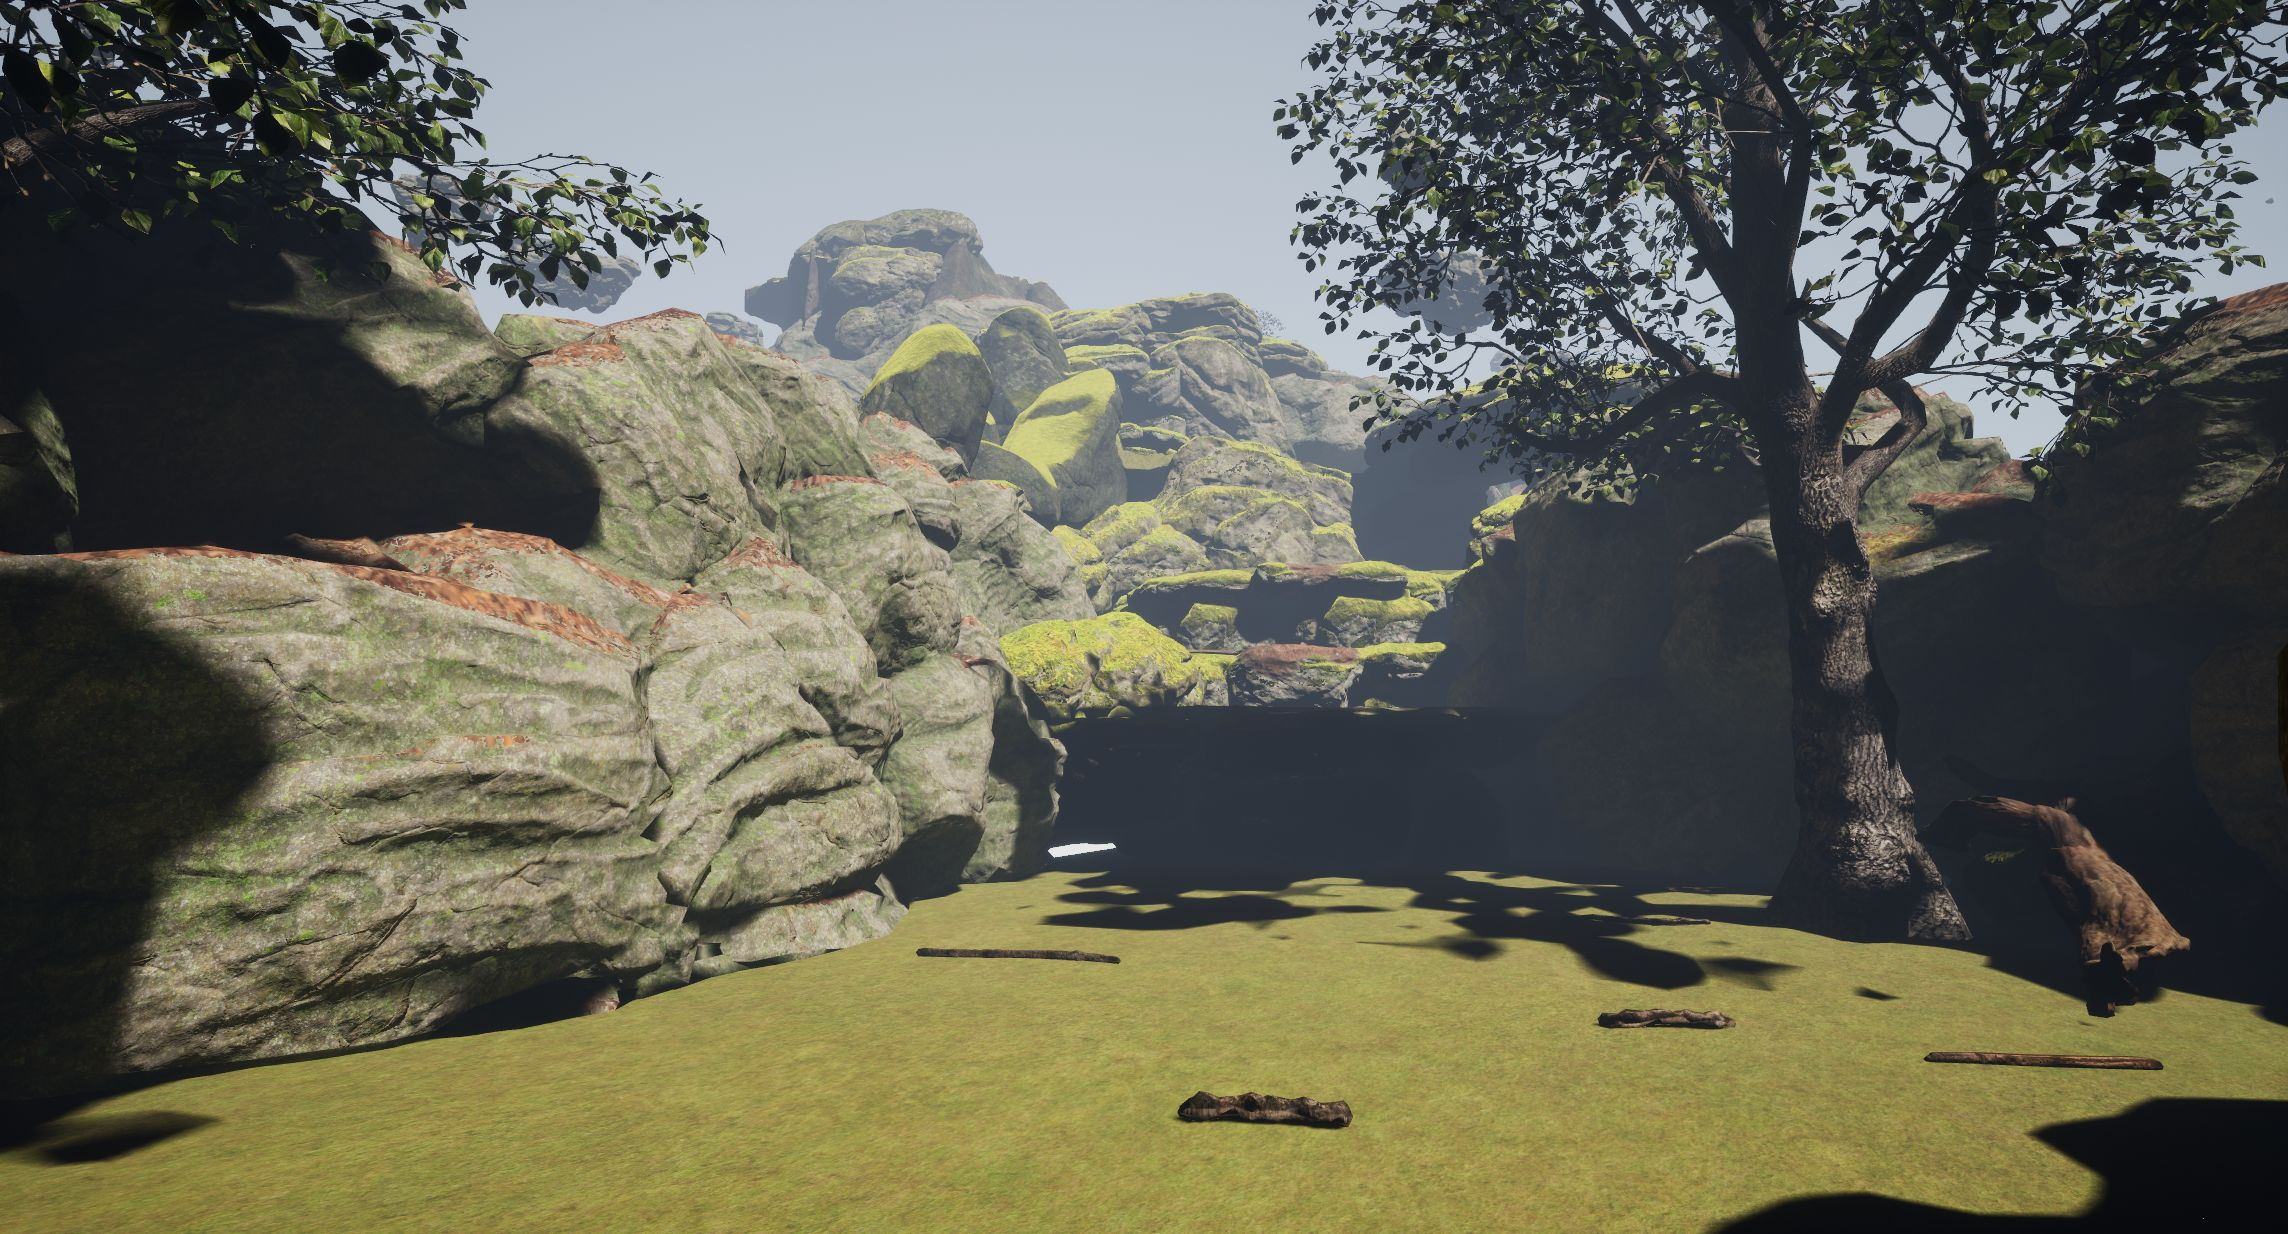
\includegraphics[width=0.9\textwidth]{images/07cha_14_complexTestCase02Environment.jpg}} \\
		\multicolumn{3}{c}{(a)} \\[6pt]	%vertical extra spacing (4 points)
		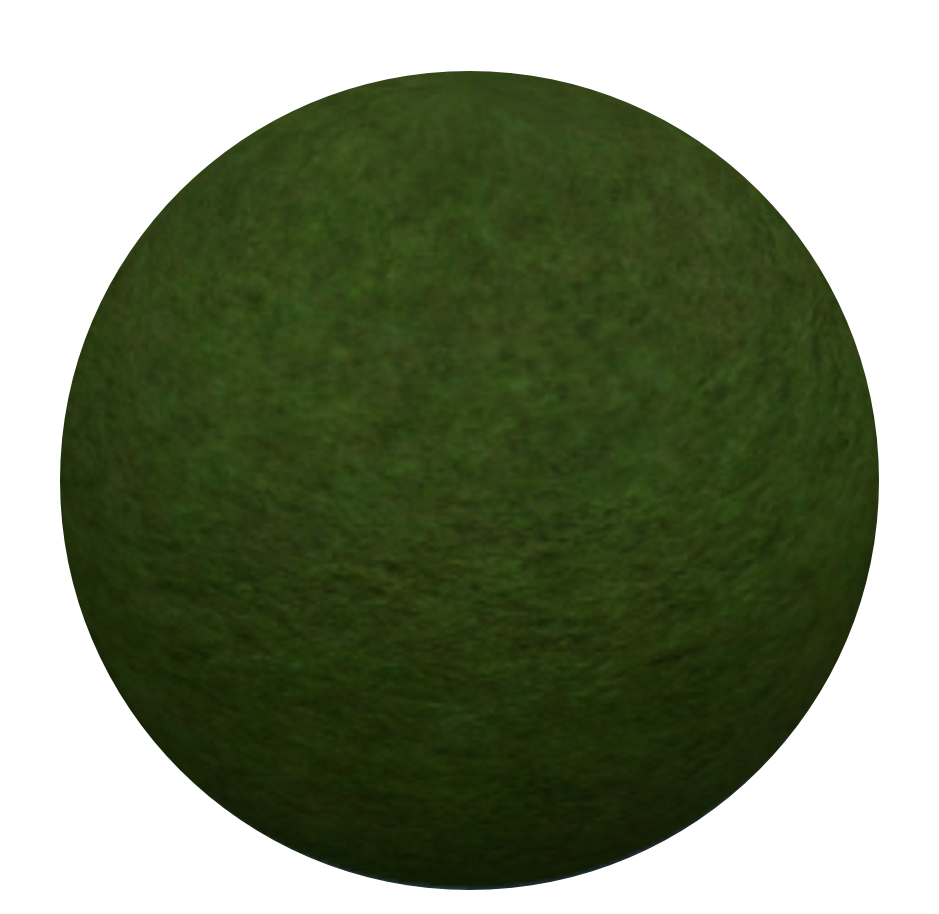
\includegraphics[width=.3\textwidth]{07cha_materialHub_grass.jpg} &
		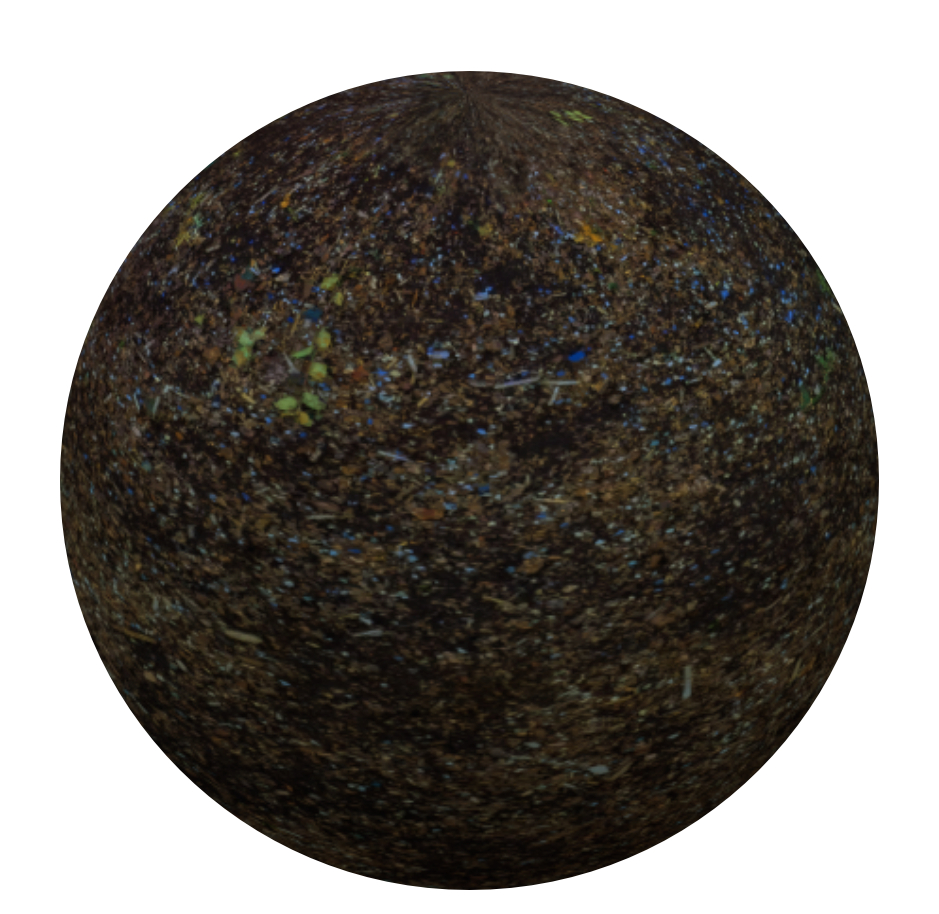
\includegraphics[width=.3\textwidth]{07cha_materialHub_ground.jpg} &
		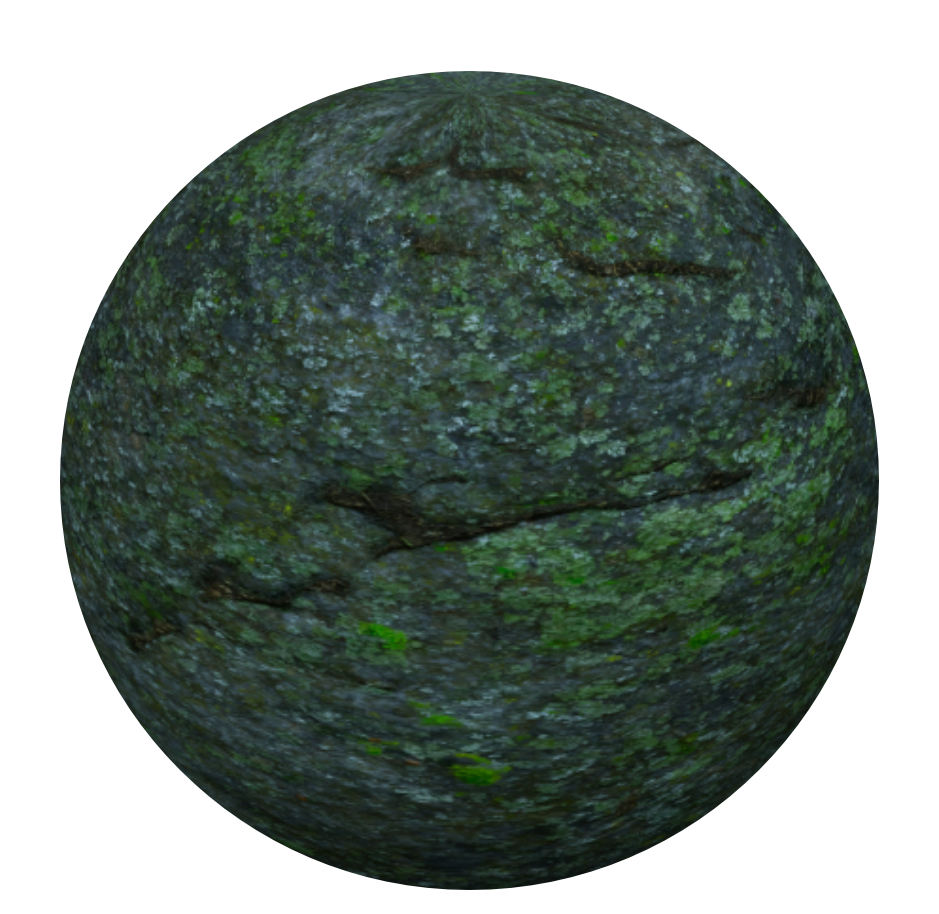
\includegraphics[width=.3\textwidth]{07cha_materialHub_rock.jpg} 	\\
		(b) & (c) & (d) \\
	\end{tabular}
	\caption{ An exterior scene from \emph{Letzte Worte}. This scene uses mainly these base Materials: grass (b), forest ground(c) and rock (d). }
	\label{fig:granularityBase}
\end{figure}


\subsubsection{\patGranularityVariation}\label{\patGranularityVariation}
\begin{description}
	\item[\patIntent:]% 
	Rather than creating a set of different generic base materials representing distinctive surface types, create variations of more complex material. 
	%\item[\patAlsoKnownAs:]% 
	\item[\patMotivation:]% 
	For instance, you want to create a kitchen scene. The walls are covered with ceramic tiles. Some areas that are often used should appear dirties and have small damages while other areas are supposed to look newer. To do so, you can create both a new  and clean version as well as an aged, slightly damaged and dirtier one of the same base material. This enables you to have more surface variety within the materials than by combining generic base materials. Further, consider a cobblestone surface which could be recreated by combing stone, mud, wood chunks, dirt and moss as base materials. Instead of combing them within the engine, they are baked into textures and tiled across the surface area. Material layering is afterwards used to create additional variations of this material. 
	\item[\patApplicability:]\hfill
	\begin{itemize}\mynobreakpar
		\item The surface is extremely complex and composed of a huge variety of different surface types.
		\item The purpose of the material layering system is to create a variety of the surface types rather than blending  completely different ones  (i.e., it is used to add aging and damage to certain areas).   
		\item The masking does not need to be as precise as for \emph{\patGranularityBase} (section \ref{\patGranularityBase}). Therefore, the texture resolution can be reduced. 
	\end{itemize}
	\item[\patImplementation:]% 
	This approach can easily be used with all pattern layering methods. 
	\item[\patExamples:]% 
	The first interior location in \emph{Letzte Worte} (see \ref{fig:granularity}) uses white wood material across all doors and windows. Initially, I split the surface into its distinctive surface types. The mask resolution was huge to achieve all the fine details, like for instance scratches. Instead of splitting the surface by the surface type, I later created two variations of the white wood material, a clean and a damaged one. This results in a highly decreased mask resolution, compared to before. The texture atlas uses only a texture resolution of 1024 by1024 pixel for the final scene, containing the mask for two doors and two windows.
	\item[\patConsequences:]\hfill 
		\begin{description}
			\item[\visual:]\hfill
			\begin{itemize}\mynobreakpar
				\item This approach allows to have more distinctive surface types than using \emph{\patGranularityBase} (section \ref{\patGranularityBase}).
				\item Different aging or damaging stages of a material can be defined and blendend afterwards.
			\end{itemize}
			\item[\performance:]\hfill
			\begin{itemize}\mynobreakpar
				\item This method requires less but more complex base materials in comparison to \emph{\patGranularityBase} (section \ref{\patGranularityBase}).
				\item The masking resolution can probably be reduced highly as it is rather used for masking out areas instead of creating transition between distinctive surface types. 
			\end{itemize}
			\item[\pipeline:]\hfill
			\begin{itemize}\mynobreakpar
				\item Base materials are more specific and can be used across less different objects. 
				\item This approach can be used with basically all pattern layering systems. 
				\item It does most likely built on texture data input. 
			\end{itemize}
		\end{description}
	\item[\patRelations:]% 
	In addition to \emph{\patGranularityBase} (section \ref{\patGranularityBase}), this pattern presents an option in how to split your surface into different base materials.
\end{description}

\begin{figure}
	\centering\small 
	\begin{tabular}{@{}cc@{}} % mittlerer Abstand = 12mm
		\multicolumn{2}{c}{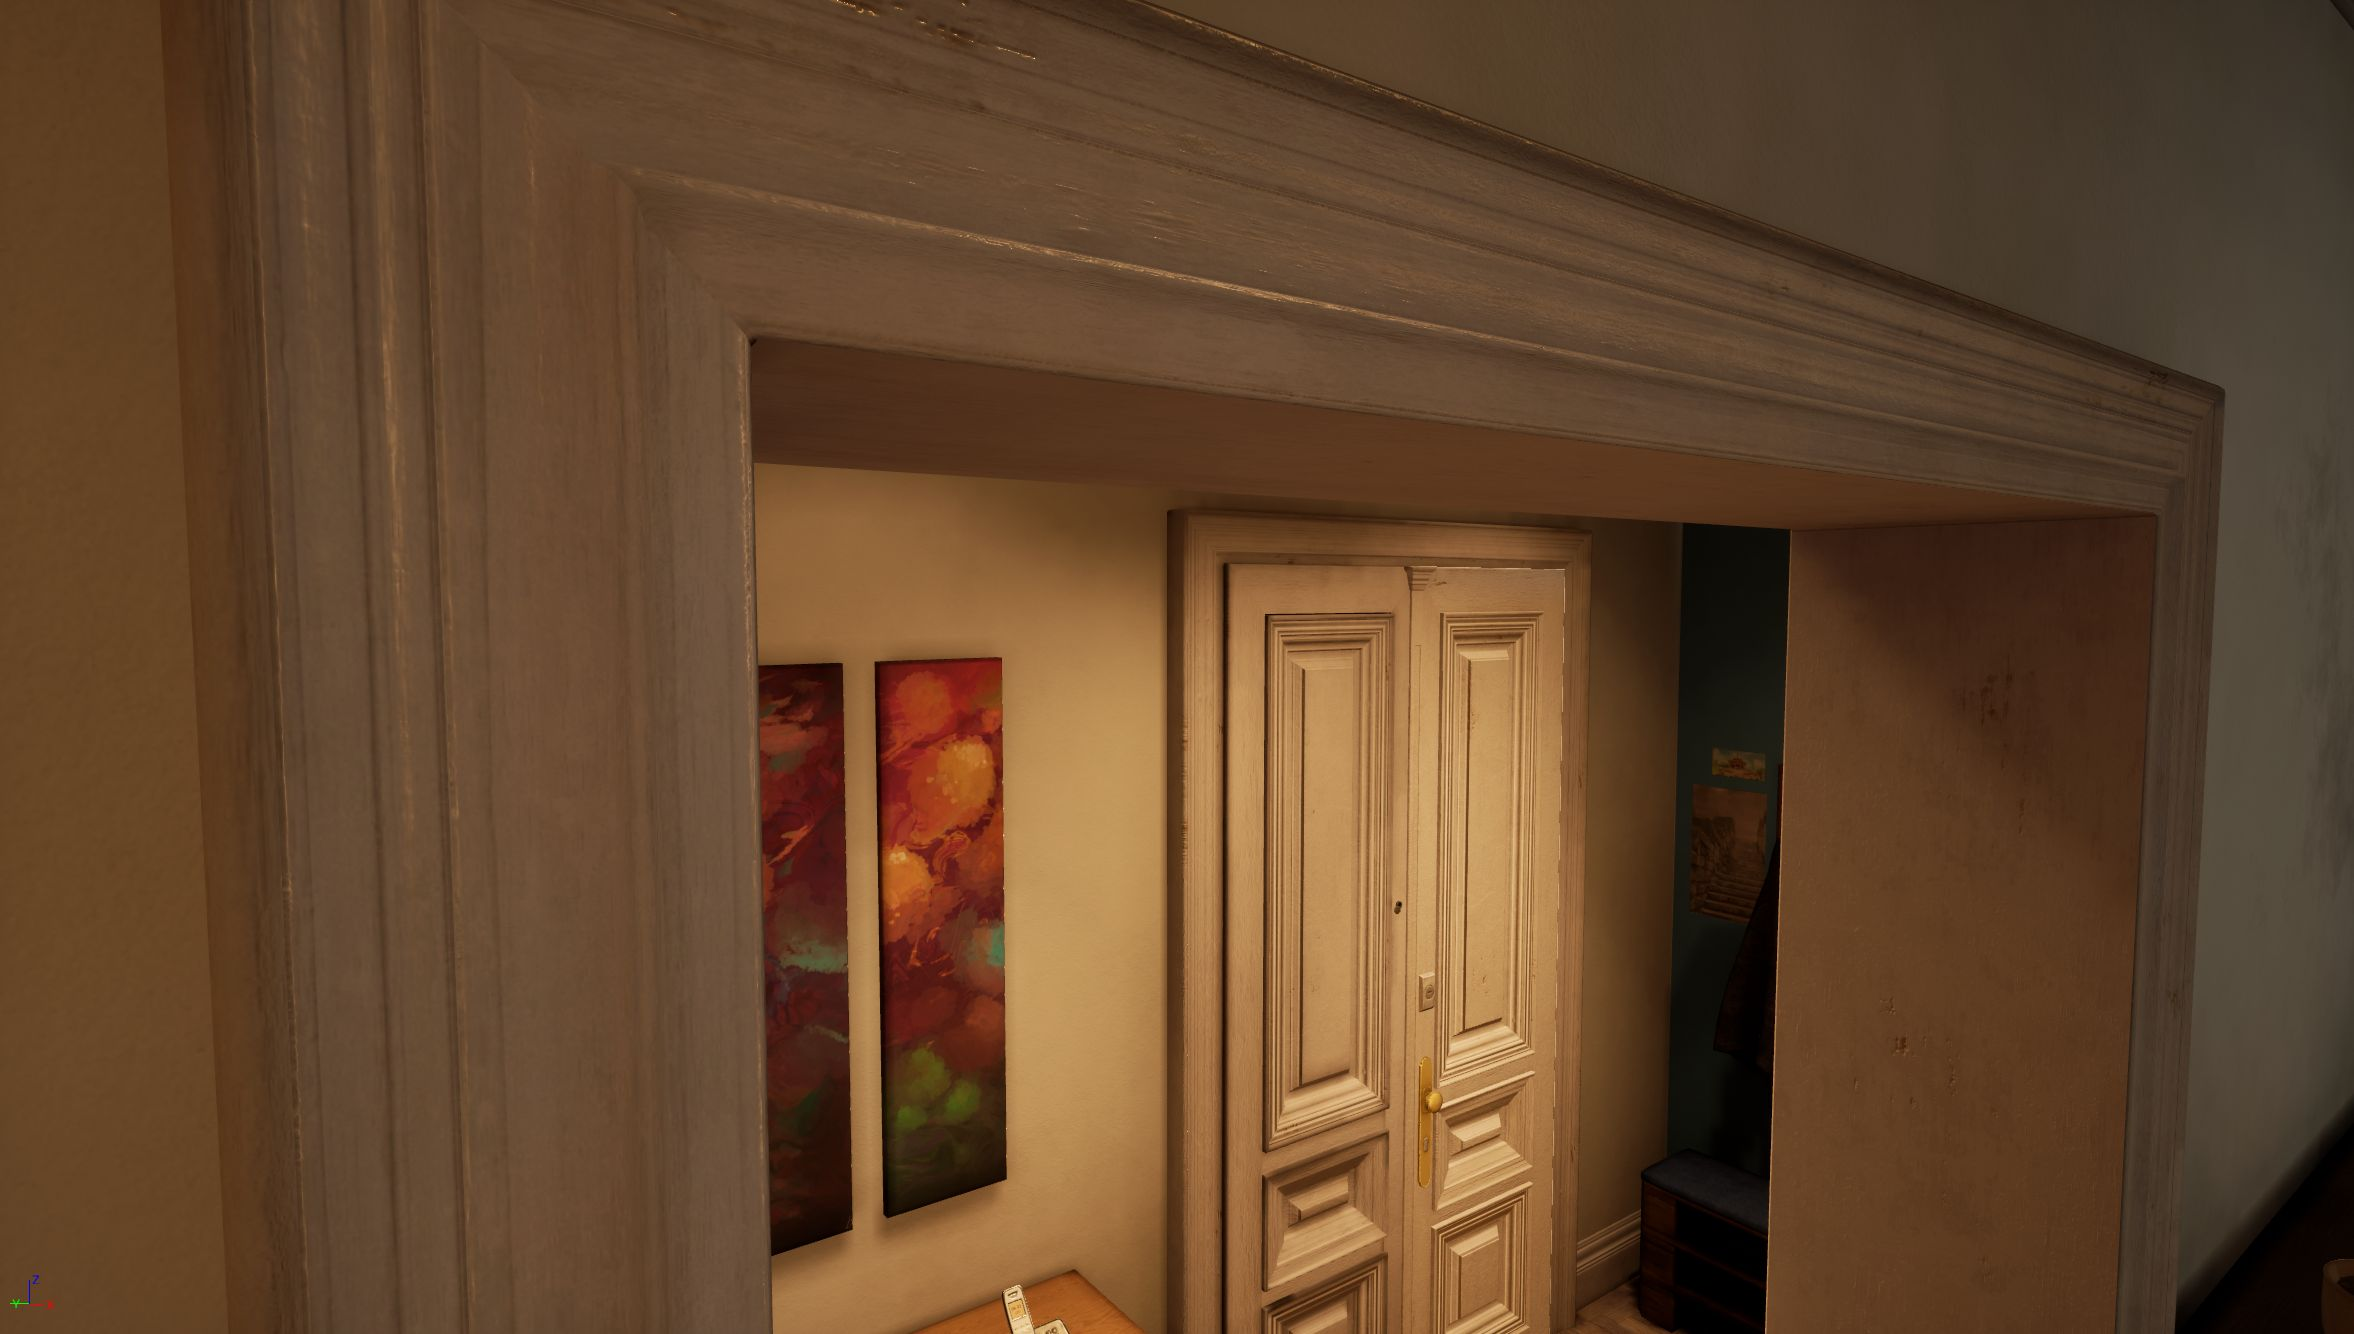
\includegraphics[width=0.75\textwidth]{images/07cha_15_LeaDoor_2.jpg}} \\
		\multicolumn{2}{c}{(a)} \\[6pt]	%vertical extra spacing (4 points)
		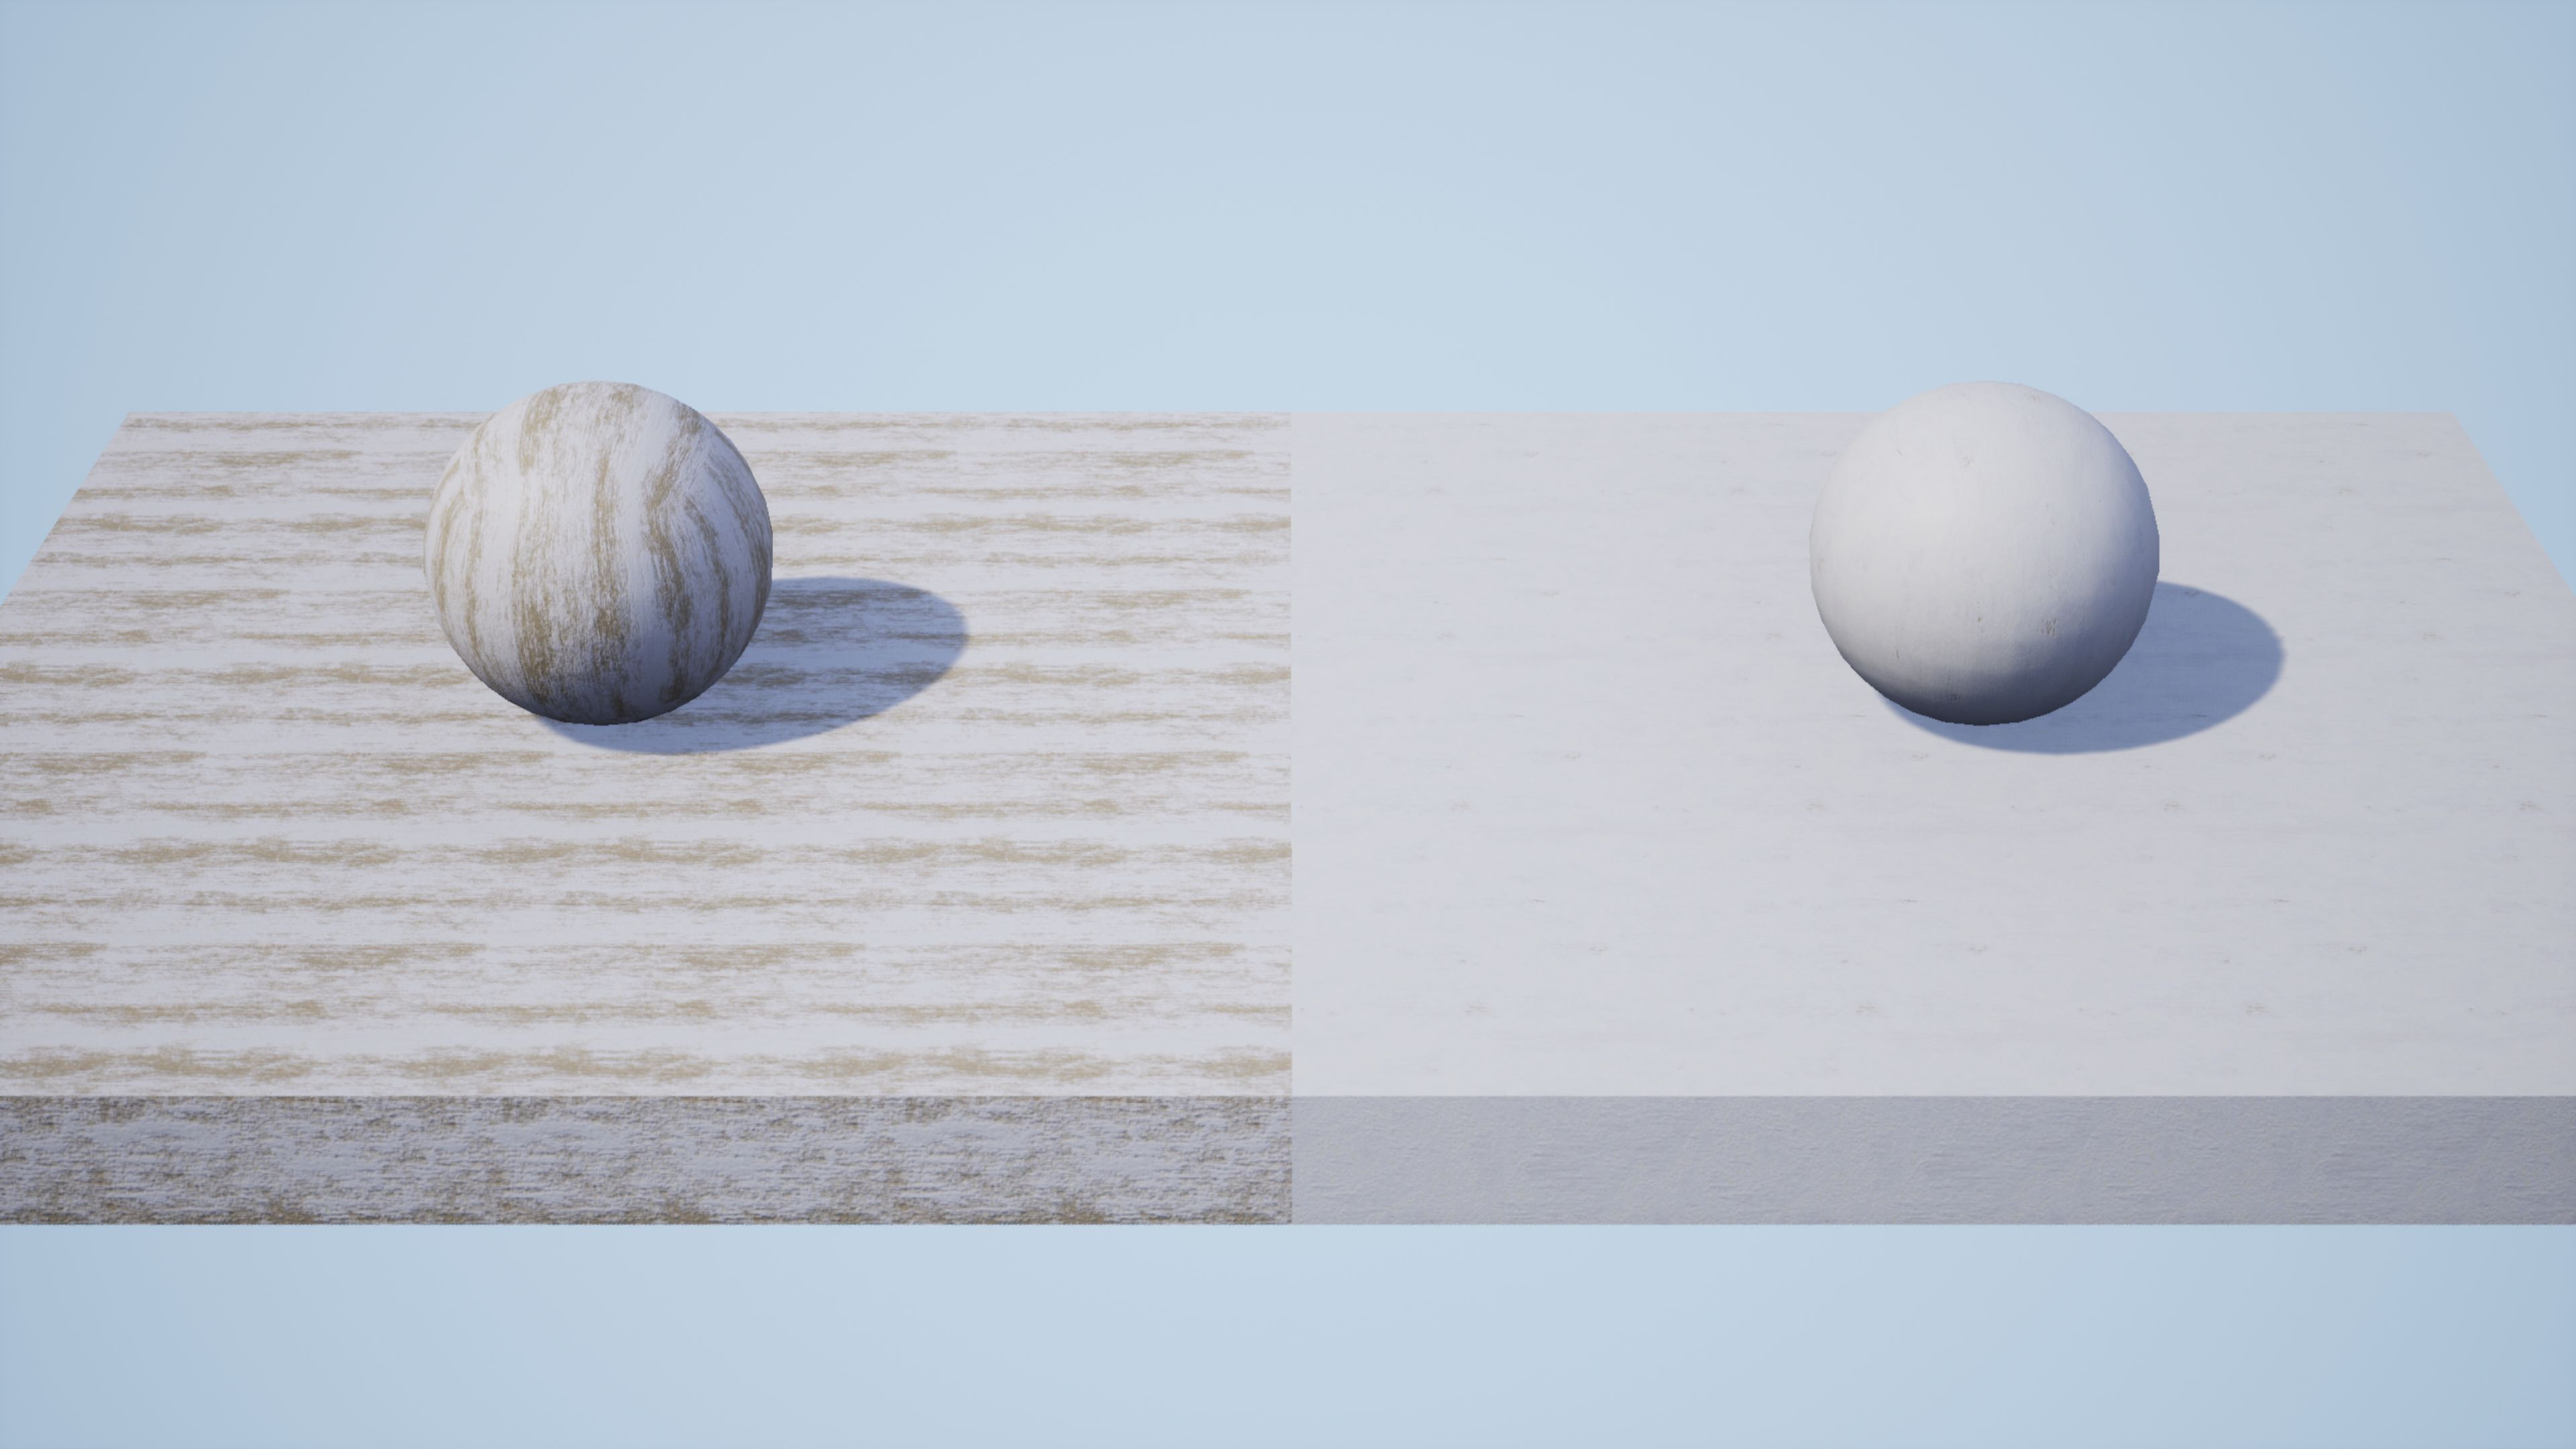
\includegraphics[width=.475\textwidth]{07cha_15_StarterMapMaterial.jpg} &
		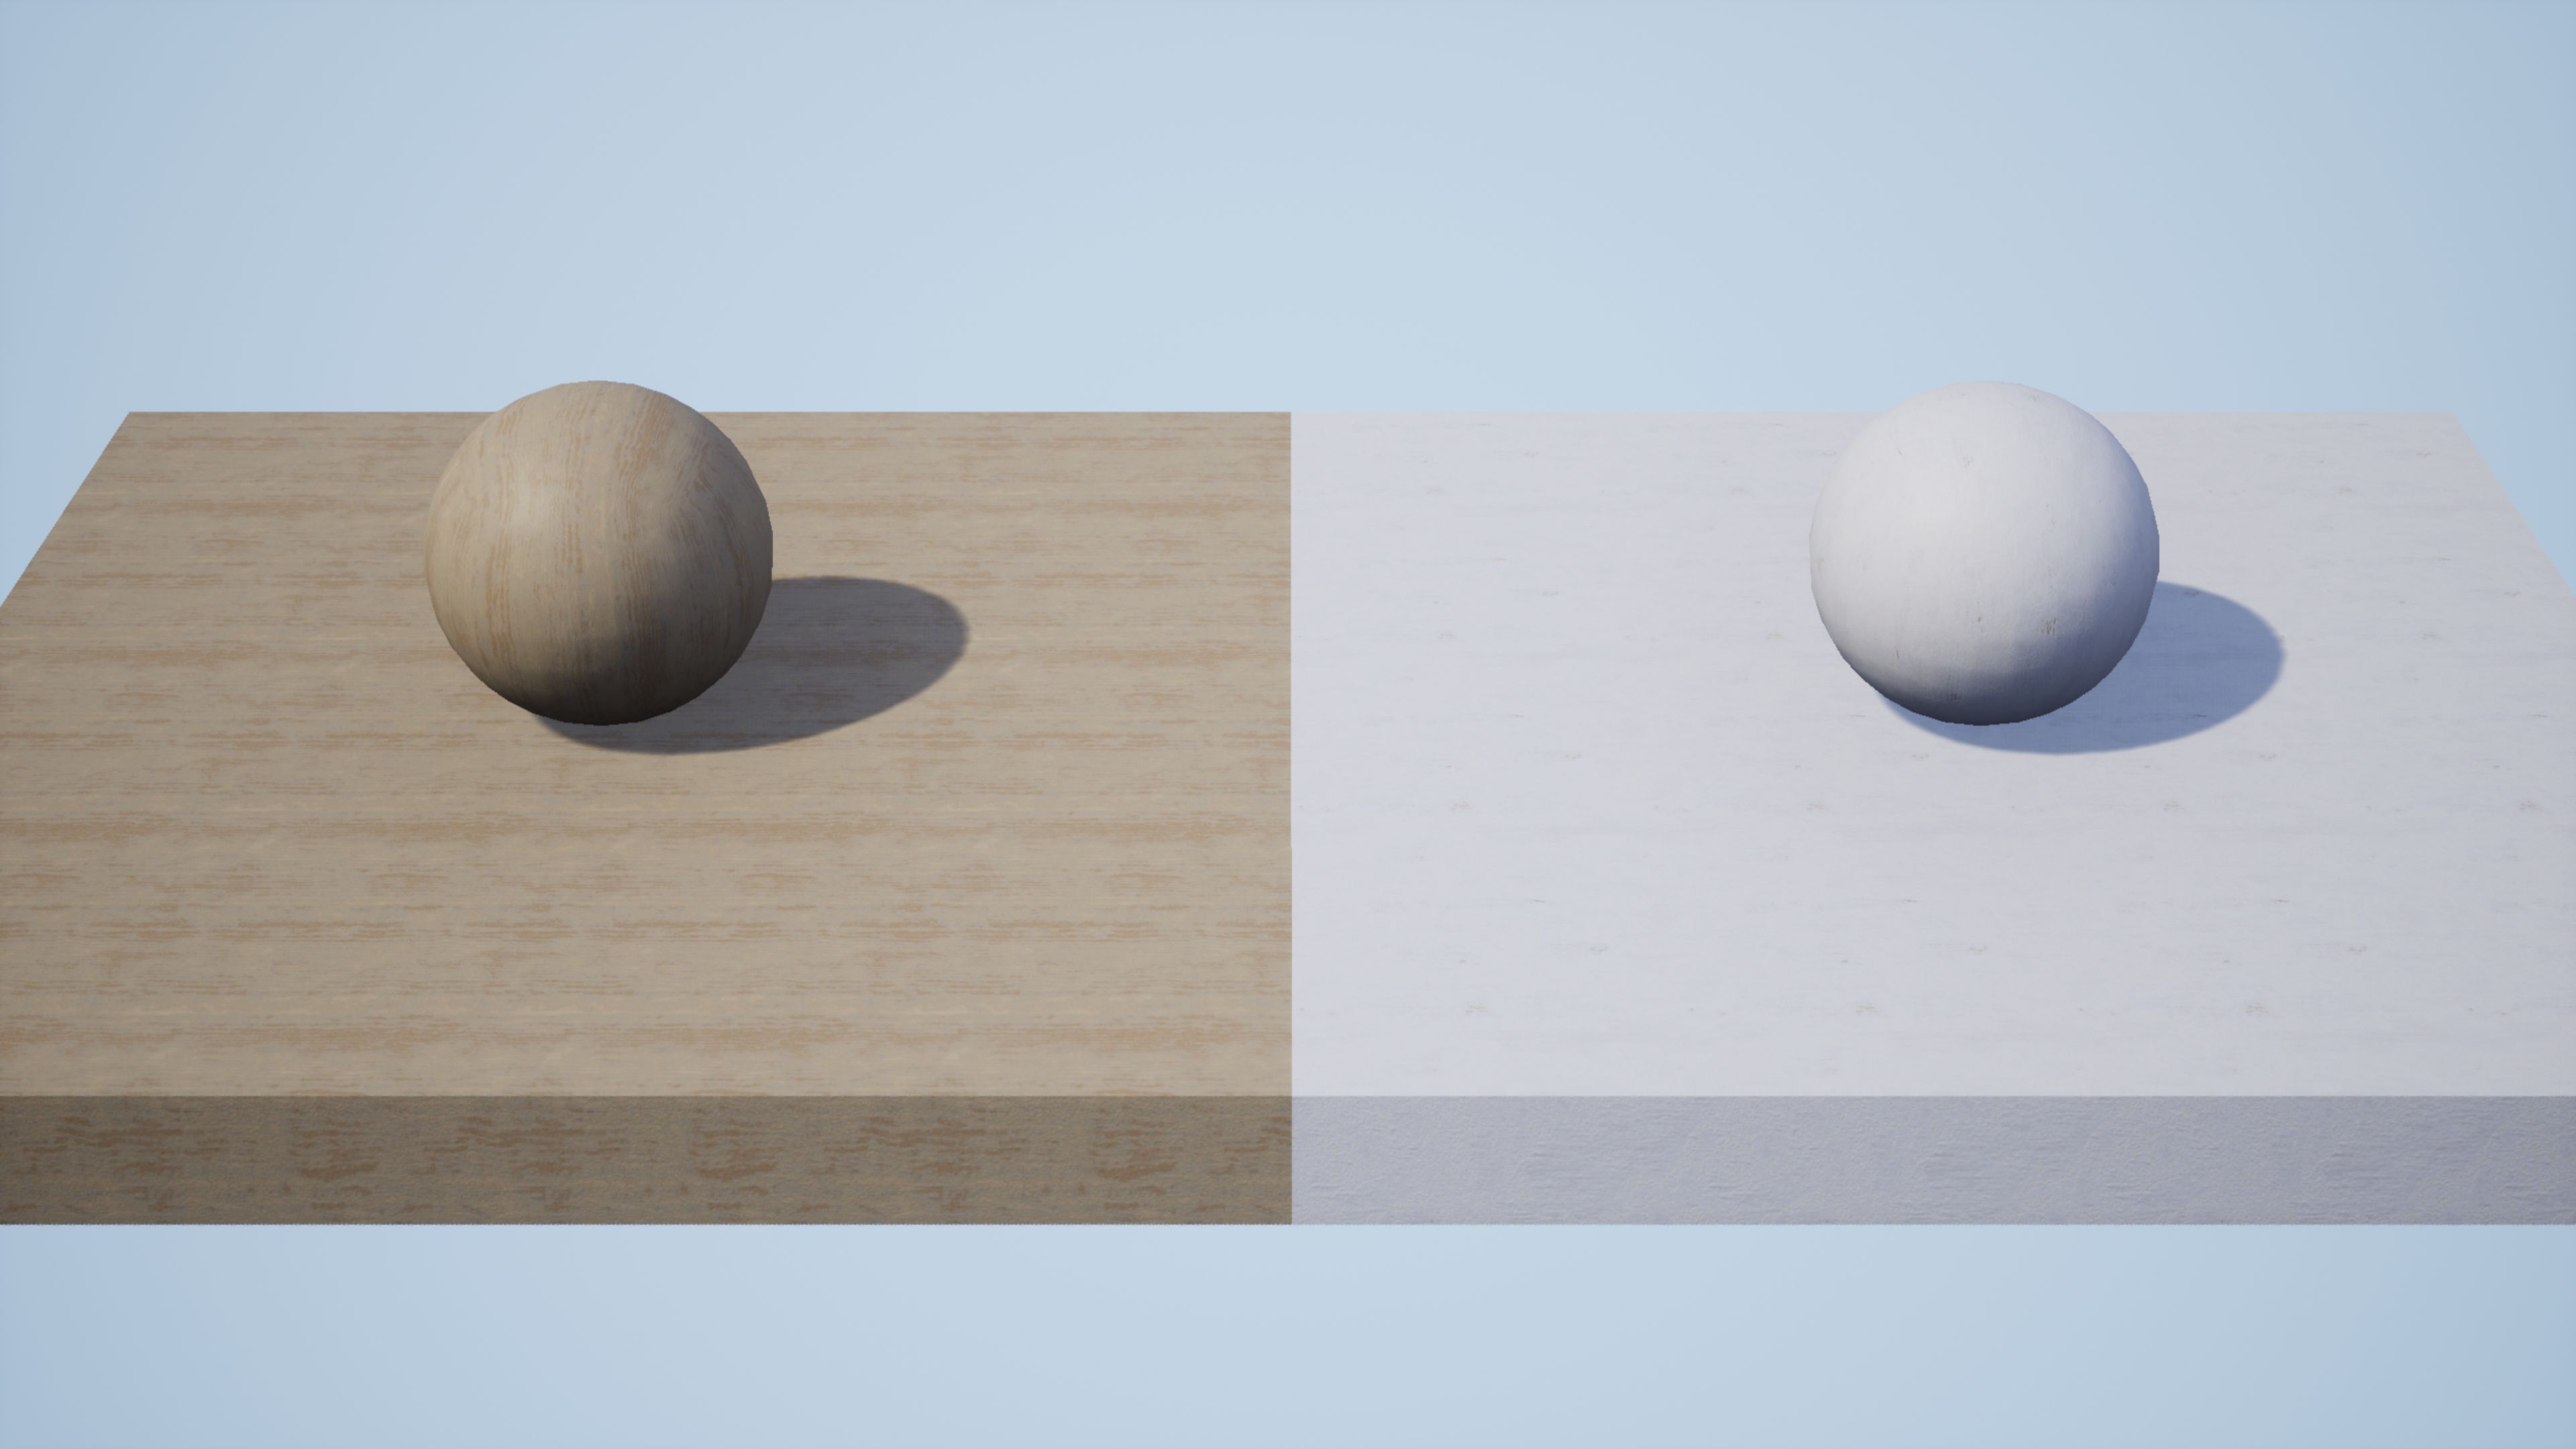
\includegraphics[width=.475\textwidth]{07cha_15_StarterMapMaterial02.jpg} 
		\\
		(b) & (c) 
	\end{tabular}
	\caption{
		Splitting a complex surface into either distinctive surface types or material variations.	Figure (a) shows the final scene from \emph{Letzte Worte}. The doors are made by blending material variations as seen in figure (b) rather than by combining two completely different surface types as seen in figure (c).}
	\label{fig:granularity}
\end{figure}



%%%%%%%%%%%%%%%%%%%%%%%%%MATERIAL CONTAINER COMPLEXITY%%%%%%%%%%%%%%%%%%%%%%%%%%%%%%%%%%%%%%%

\subsection{\patCatComplexity}\label{\patCatComplexity}

The patterns proposed in this category help you to define how much complexity and data you want to put into a material container. Does every material container represent a fully described material layer object defining all surface properties? Can material containers be used to describe only a few material properties? \emph{\patComplexityFulMaterial} (section \ref{\patComplexityFulMaterial}) and \emph{\patComplexitMaterialModulation} (section \ref{\patComplexitMaterialModulation}) compare these two distinctive workflows and will help you decide where to use which one. These patterns are closely connected to the patterns in category \emph{\patCatBlending}: \emph{\patBlendingFull} (section \ref{\patBlendingFull})and \emph{\patBlendingPartially} (section \ref{\patBlendingPartially}). The design of the \emph{\patCatBlending} needs to provide the functionality for either blending only certain material properties or not. Section \ref{sec:blendingModes} contains further details how this decision is closely connected to the blending module.   

\subsubsection{\patComplexityFulMaterial}\label{\patComplexityFulMaterial}
\begin{description}
	\item[\patIntent:]% 
	Create a base material by specifying all material parameters (e.g., base color, roughness, metalness) so that it fully represents a real world surface.
	%\item[\patAlsoKnownAs:]% 
	\item[\patMotivation:]% 
	You use a physically plausible blending workflow as presented in pattern \emph{\patBlendingFull} (section \ref{\patBlendingFull}). You specify base materials that represent real word surfaces and blend those. 
	\item[\patApplicability:]% 
	The intent is to work in a physically plausible way. Real world surfaces are composed of different surface types. Creating base materials that describe the entire material properties of a certain surface type corresponds best to this idea.
%	\begin{itemize}
%		\item The intent is to work in a physically plausible way. Real world surfaces are composed of different surface types. Creating base materials that describe the entire material properties of a certain surface type corresponds best to this idea. 
%	\end{itemize}
	\item[\patImplementation:]% 
	This approach can be used with all pattern layering systems. 
	%\item[\patExamples:]% 
	\item[\patConsequences:] 
	\begin{description}
		\item[\visual:]\hfill
		\begin{itemize}
			\item The number of different base materials is highly limited as every one contains full surface description data. 
			\item The results of blending two base materials with one another are predictable and therefore artist friendly. 
			\item The workflow is intuitive if you are used to decomposing an object into different base materials (e.g., a metal, partially covered with rust, paint and dirt)
			\item The artistic process is much freer than \emph{\patComplexitMaterialModulation} (section \ref{\patComplexitMaterialModulation}) as blending behaves consistently. Besides, you don't have to worry about how to blend which individual material parameter. 
		\end{itemize}
		\item[\performance:]\hfill
		\begin{itemize}
			\item Blending many similar base materials may result in blending similar roughness or normal values. By providing more control, this texture count could be reduced without a significant impact on the visual quality. 
		\end{itemize}
		\item[\pipeline:]\hfill
		\begin{itemize}
			\item The blending between different base materials behaves in a consistent way. 
			\item The structure of all base materials is consistent. This makes it easy to change and replace them.  
		\end{itemize}
	\end{description}
	%\item[\patRelations:]% 
\end{description}



. 
\subsubsection{\patComplexitMaterialModulation}\label{\patComplexitMaterialModulation}

\begin{description}
	\item[\patIntent:]% 
	Enabling material containers to specify only a few material properties instead of all makes them more lightweight but less predictive.
	%\item[\patAlsoKnownAs:]% 
	\item[\patMotivation:]% 
	The amount for blending fully described base materials is limited to only a few. To increase the number of base materials that can be blended a more flexible way of defining material containers is used. Instead of blending four wood base materials, all fully described with all parameters, you can blend two fully described base materials with partially described ones. Latter are used to modulate the roughness and replace the base color channel. This decreases the texture count from twelve (three per base material) to eight. 
	\item[\patApplicability:]\hfill
	\begin{itemize}\mynobreakpar
		\item You want more flexibility in if and how to blend the individual material parameters.
		\item The amount of layers can be decreased by reducing the complexity of individual base materials and the blending process. 
	\end{itemize}
	\item[\patImplementation:]% 
	This approach requires the ability to influence the shader or shading system. It is therefore not viable for \emph{\patImplementationBUildtIn} (section \ref{\patImplementationBUildtIn}). It also requires more control over the actual blending process. With this approach, a material container does not represent an entire surface but only certain properties. It will therefore not work for pattern layering shaders or systems that target a physically plausible blending, \emph{\patBlendingFull} (section \ref{\patBlendingFull}). For this pattern to work, a pattern layering system is required that uses the following patterns: \emph{\patImplementationCustomShader} (section \ref{\patImplementationCustomShader}), \emph{\patBlendingPartially} (section \ref{\patImplementationCustomShader}) and \emph{\patWorkflowIndividualShader} (section \ref{\patWorkflowIndividualShader}) or \emph{\patWorkflowContentDrivenShader} (section \ref{\patWorkflowContentDrivenShader}).
	\item[\patExamples:]%
	Figure \ref{fig:learoomwallmodulation} shows an interior location from \emph{Letzte Worte}. The wall shader is composed of different layers: the main plastered wall, some rougher wall and three painted wall layers. These painted wall layers do not contain a full base material: they only include a base color and a value to adjust the roughness.  
	\item[\patConsequences:]\hfill 
		\begin{description}
			\item[\visual:]\hfill
			\begin{itemize}\mynobreakpar
				\item This approach allows to use more layers, especially if the distinctive base materials are supposed to be really similar. 
				\item The considerations of how to blend which parameters, while considering the trade-offs between using certain material parameters or not, might hinder the artistic process. 
			\end{itemize}
			\item[\performance:]\hfill
			\begin{itemize}\mynobreakpar
				\item Describing and blending base materials only partially makes them more lightweight. 
			\end{itemize}
			\item[\pipeline:]\hfill
			\begin{itemize}\mynobreakpar
				\item This introduces an additional stage within the pipeline and increases shading and pipeline complexity. 
				\item The shader or shading system does require to fit certain defined criteria, further explained above in Implementation.
			\end{itemize}
		\end{description}
	\item[\patRelations:]% 
	For this pattern to work, the blending module requires to be designed according to pattern \emph{\patBlendingPartially} (section \ref{\patBlendingPartially}).
\end{description}

\begin{figure}
	\centering
	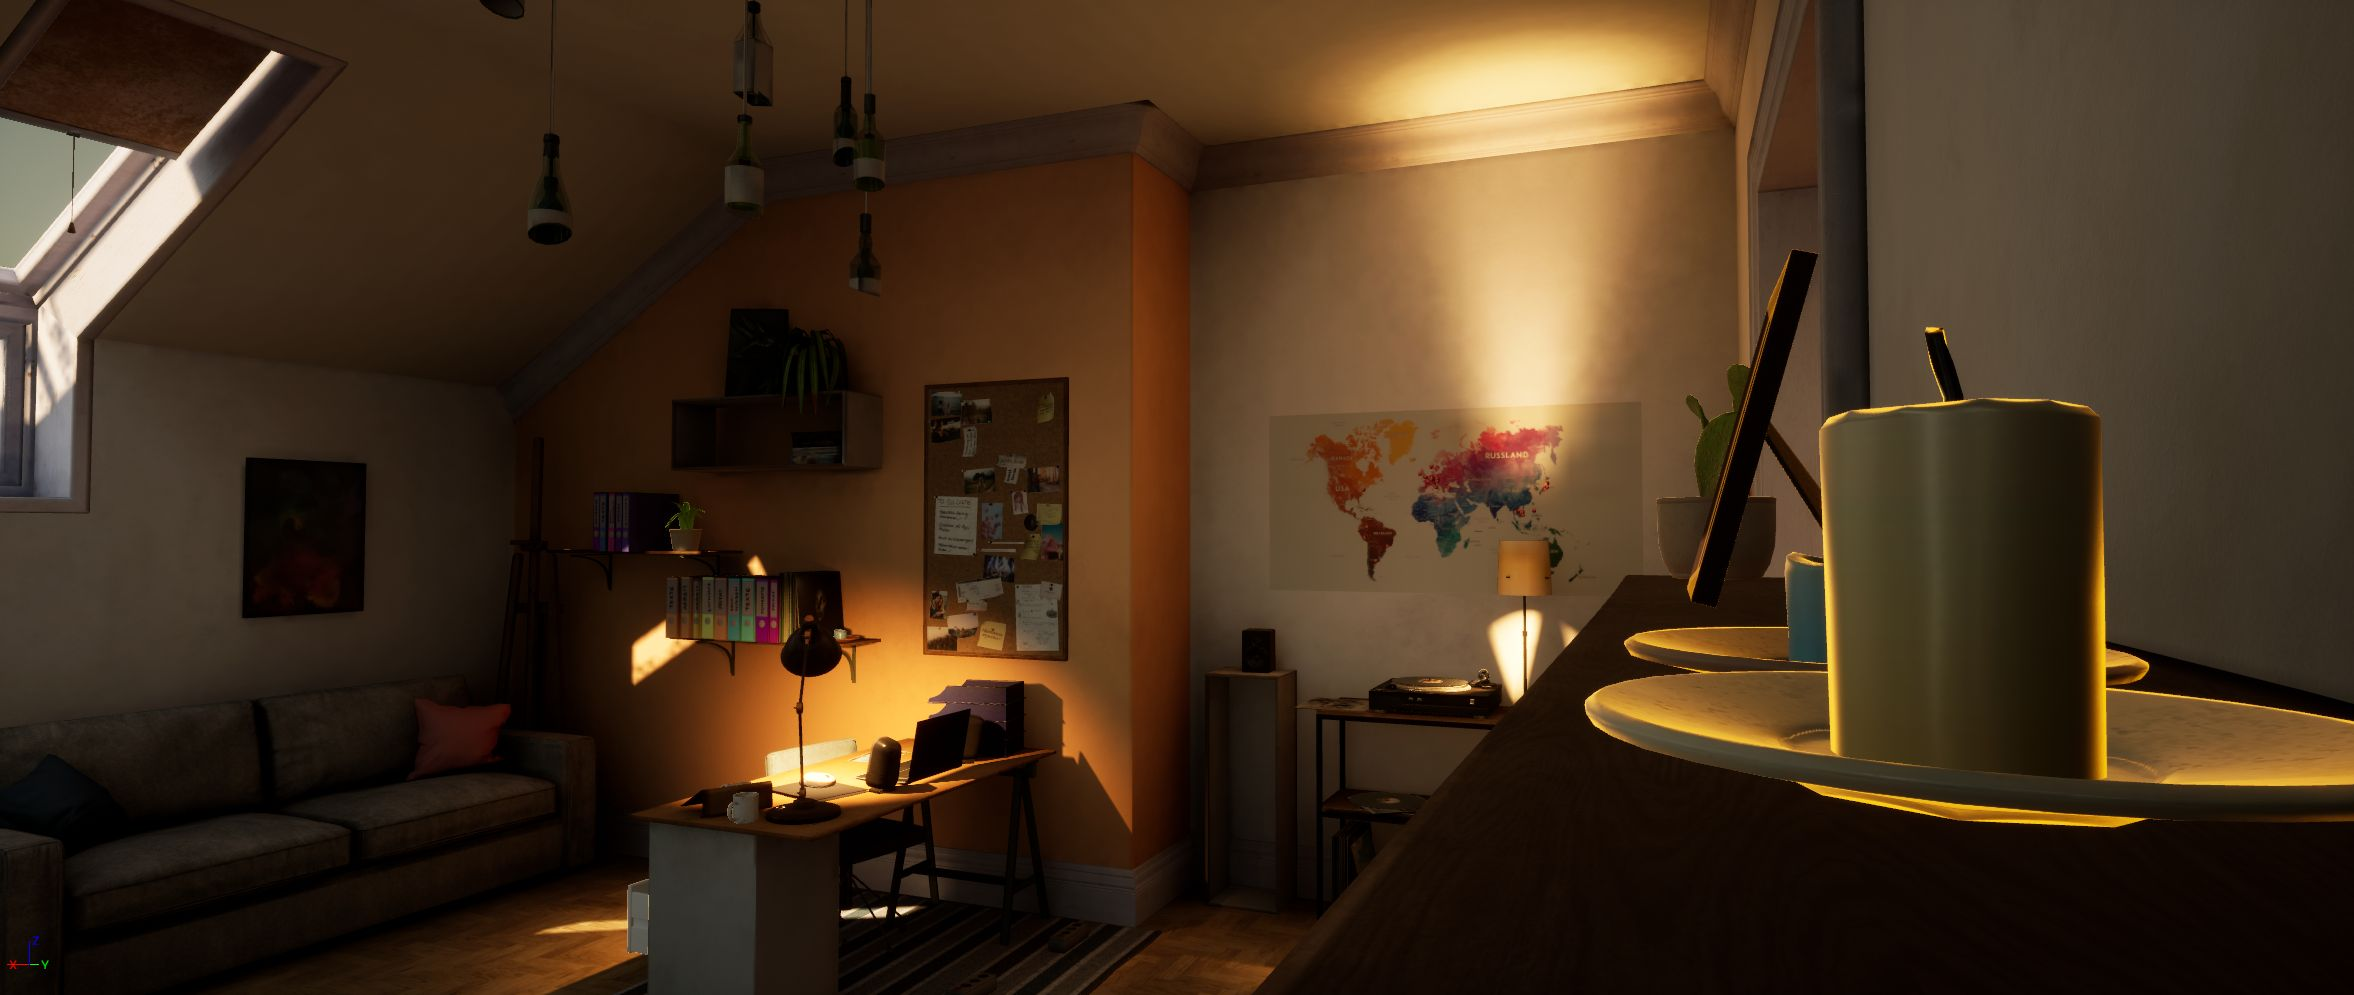
\includegraphics[width=0.9\linewidth]{images/07cha_16_leaRoomWallModulation.jpg}
	\caption{ Blending partially described base materials to create surface variaty in \emph{Letzte Worte}. The orange wall does not use a full base material description. It defines only individual properties to modulate the previous base material.}
	\label{fig:learoomwallmodulation}
\end{figure}


%%%%%%%%%%%%%%%%%%%%%%%%%MATERIAL CONTAINER CREATION%%%%%%%%%%%%%%%%%%%%%%%%%%%%%%%%%%%%%%%

\subsection{\patCatCreation}\label{\patCatCreation}

The following patterns support you in defining the creation process of individual base materials. I decided to categorize them into \emph{\patCreationInputDefined} (section \ref{\patCreationInputDefined}) and \emph{\patCreationProcedural} (section \ref{\patCreationProcedural}). In the former, the material properties are defined by the inputs without much additional computation (e.g., texture maps defining roughness, metalness and base color). The latter uses different inputs to drive procedural material creation (e.g., color tint based on world position). This decision has huge impact on the pipeline and way of working with base materials. These patterns can also be combined to achieve the desired result.  

\subsubsection{\patCreationInputDefined}\label{\patCreationInputDefined}
\begin{description}
	\item[\patIntent:]% 
	The surface properties of the base material are mostly defined by its inputs. There is limited to no manipulation of this data before passing it on to the shader or next component within the material layering module. 
	%\item[\patAlsoKnownAs:]% 
	\item[\patMotivation:]% 
	You define the surface properties of the base materials within any 3rd party painting tool. After exporting, importing and assigning them to the right materials, you just want it to look the same as in the authoring tool.  
	\item[\patApplicability:]\hfill 
	\begin{itemize}\mynobreakpar
		\item This works best in combination with other texture authoring applications. 
		\item Values are set by either using textures or parameters.
		\item The result is predictable, highly controllable and well supported.  
	\end{itemize}
	\item[\patImplementation:]% 
	An input defined base material creation is supported by any pattern layering implementation or workflow. Shaders using \emph{\patImplementationBUildtIn} (section \ref{\patImplementationBUildtIn}) require most likely input defined base materials. 
	\item[\patExamples:]% 
	The interior room from \emph{Letzte Worte} in figure \ref{fig:complextestcase01room} uses mostly texture inputs for the definition of the base materials. Only a few objects use procedural shading, e.g., the color bottles, tubes and folders use procedural color randomization. 
	\item[\patConsequences:]\hfill
	\begin{description}
		\item[\visual:]\hfill
			\begin{itemize}\mynobreakpar
				\item This provides a control over the individual properties of a base material. 
				\item Artists can focus on creating art and do not need to get technical. 
			\end{itemize}
		\item[\performance:]\hfill
			\begin{itemize}\mynobreakpar
				\item It is efficient if textures are reused across a lot of different objects. 
			\end{itemize}
		\item[\pipeline:]\hfill
			\begin{itemize}
				\item It uses an artist friendly workflow. 
				\item Texture based workflows are widely integrated in the different pipelines. 
			\end{itemize}
	\end{description}
	\item[\patRelations:]% 
	Input driven base material definition is commonly used across all pattern layering worfklows and implementations. A \emph{\patImplementationBUildtIn} (section \ref{\patImplementationBUildtIn}) is most likely limited to this input based workflow.
\end{description}

\begin{figure}
	\centering
	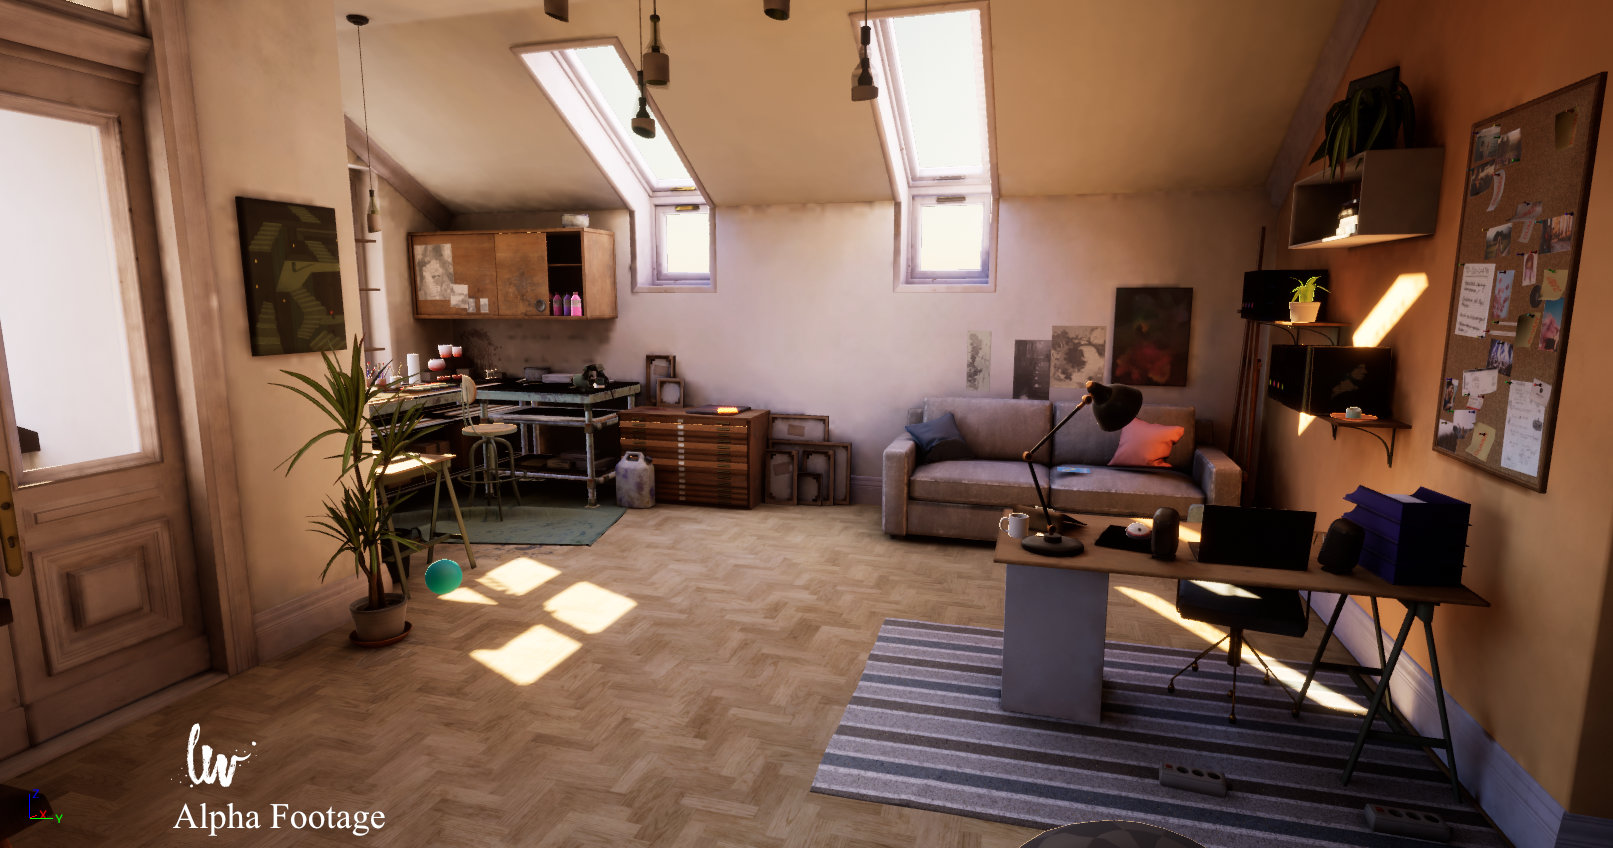
\includegraphics[width=0.9\linewidth]{images/07cha_17_complexTestCase01Room.jpg}
	\caption{A location from \emph{Letzte Worte} using mainly input defined base materials.}
	\label{fig:complextestcase01room}
\end{figure}

\subsubsection{\patCreationProcedural}\label{\patCreationProcedural}
\begin{description}
	\item[\patIntent:]% 
	Use input driven procedural methods to define and modulate the final base material properties.
	%\item[\patAlsoKnownAs:]% 
	\item[\patMotivation:]% 
	Consider a modular level kit which already uses pattern layering for shading. The same wooden wall panel asset is located several times side by side. It is noticeable that they share the same textures and UVs. An easy way to fix this is to procedurally offset the UV coordinates for the wooden base material. All masking and all other base materials stay in the same place. By offsetting the UVs on every object differently based on the shader, it is much less obvious that they share the same texture.  
	\item[\patApplicability:]\hfill 
	\begin{itemize}\mynobreakpar
		\item Pseudo randomness is wanted from within the shader. 
		\item Material properties need to interact with scene data (e.g., change of color based on scene height).
		\item The shader uses shader based vertex animation. 
		\item The shader is supposed to interact with the player or other dynamic objects (e.g., interactive grass, white foam around objects in the water).			
	\end{itemize}
	\item[\patImplementation:]% 
	The shader graph editors within \emph{Unity} and \emph{UE4} provide access to a huge variety of inputs and different operations for manipulating them. 
	\item[\patExamples:]% 
	The color tubes and bottles shown in figure \ref{fig:acrilyccolors} use the same textures. A semi procedural base material, combined with a mask, is used to randomize the color of the bottles. Additional color splatters are placed on top. The UVs for the bottles are randomized based on their world position so that each is covered differently with color splatters. This allows to generate an infinite number of distinctive color bottles by still using the same inputs for all of them. 
	\item[\patConsequences:]\hfill
		\begin{description}
			\item[\visual:]\hfill
				\begin{itemize}\mynobreakpar
					\item Procedural systems can be used to increase variety.
					\item They can be used to create a more reactive and immersive world (e.g., reacting vegetation).
					\item They can create global changes across different objects.
				\end{itemize}
			\item[\performance:]\hfill
				\begin{itemize}\mynobreakpar
					\item The performance cost depends highly on the operations and inputs used. 
					\item UV manipulations and simple mathematical operations are cheap.
					\item Recreating complex surfaces procedurally is expensive. Generally, only semi procedural methods are therefore used for creating photorealistic surfaces for real-time productions. 
				\end{itemize}
			\item[\pipeline:]\hfill
				\begin{itemize}\mynobreakpar
					\item They are easy to use with shader graph editors.
					\item Simple procedural input manipulation can be recreated manually in most content creation application like \emph{Maya} and \emph{Blender} for previewing.  
				\end{itemize}
		\end{description}

	\item[\patRelations:]% 
	Using semi procedural base material definition can be used to create huge variety, in contrast to \emph{\patCreationInputDefined} (section \ref{\patCreationInputDefined}). The inputs used are an important aspect for procedural creation. Please refer to category \emph{\patCatExternalInputs} in section \ref{\patCatExternalInputs}. The operations used are similar to those for procedural masking \emph{\patMaskingCreationProcedural} (section \ref{\patMaskingCreationProcedural}).
\end{description}




\begin{figure}
	\centering
	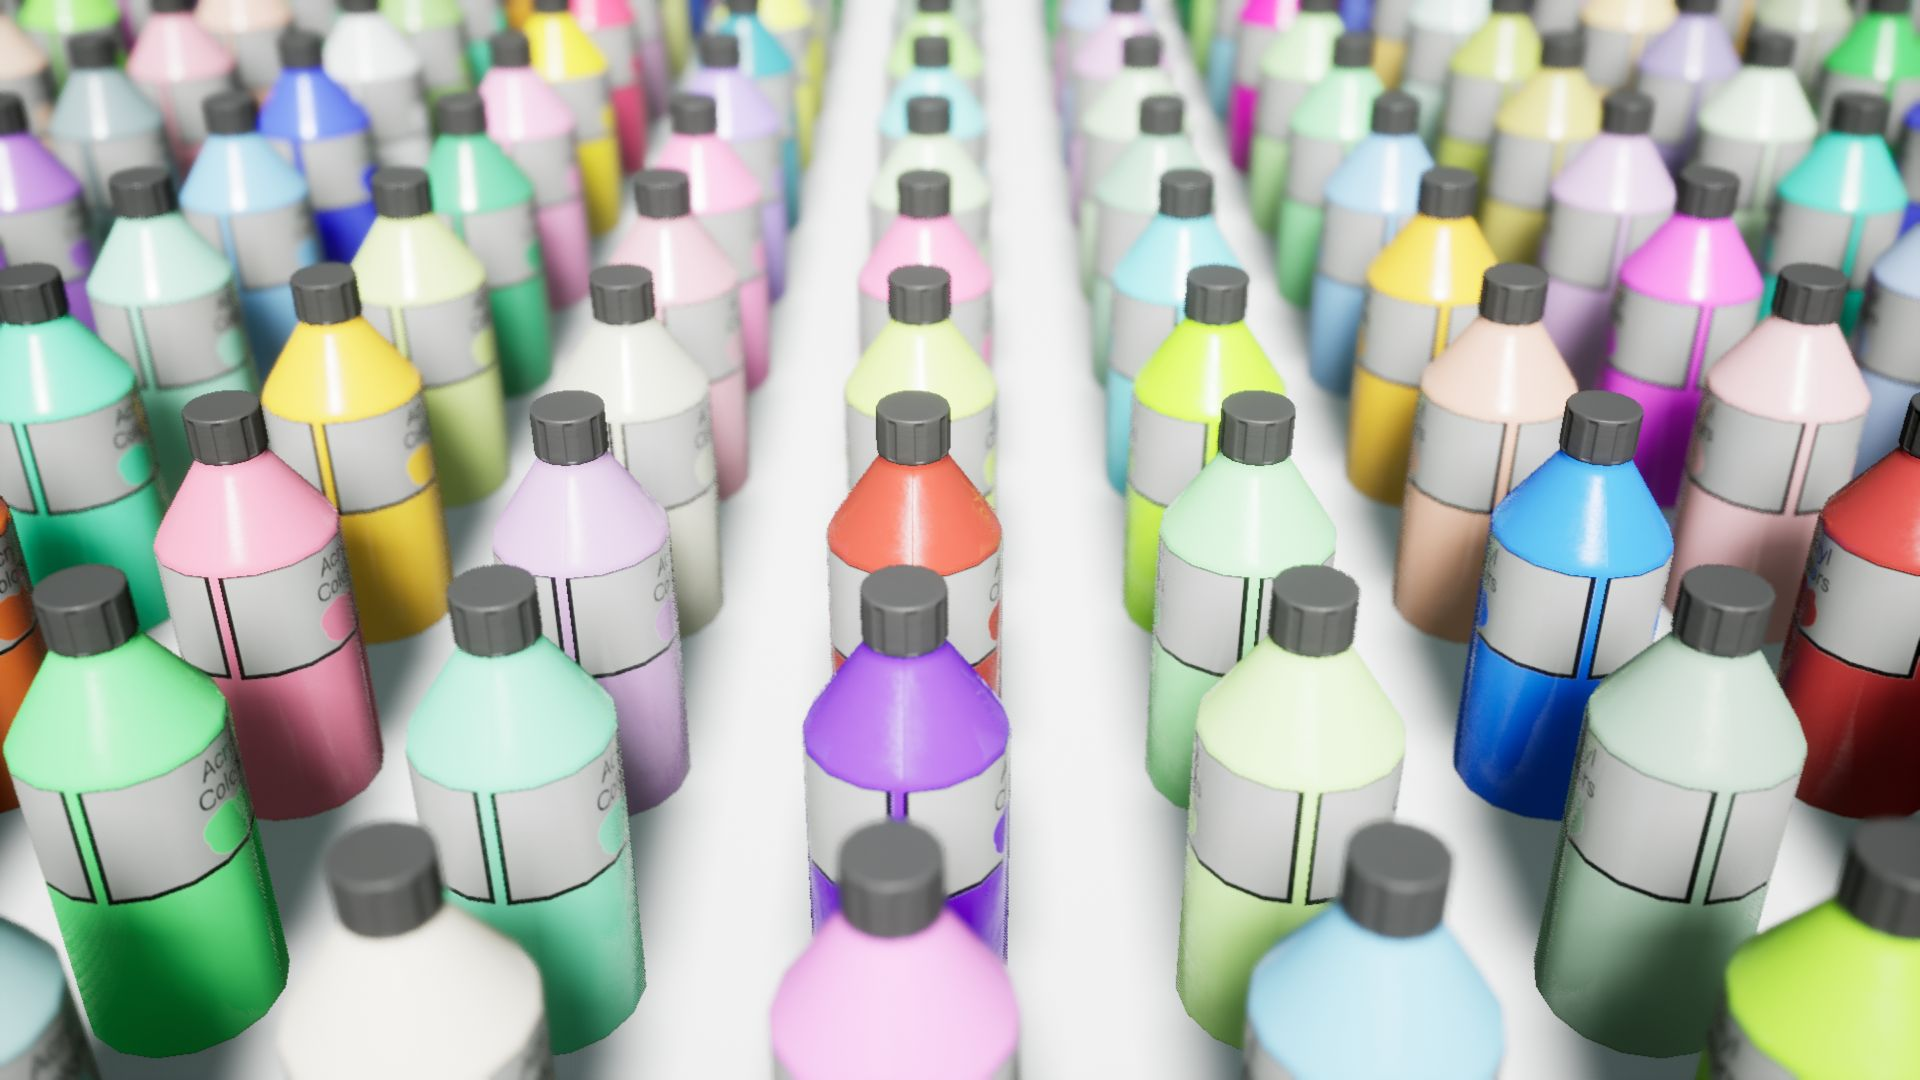
\includegraphics[width=0.7\linewidth]{images/07cha_18_acrilyc_colors.jpg}
	\caption{Procedurally modified base materials. All these color bottles share the same texture information (e.g., base color, normal, roughness). An additional mask channel is used to define the area that is procedurally modified to use a pseudo random color based on the position.}
	\label{fig:acrilyccolors}
\end{figure}


%%%%%%%%%%%%%%%%%%%%%%%%%MASKING CONTAINER%%%%%%%%%%%%%%%%%%%%%%%%%%%%%%%%%%%%%%%

\section{\patCatMaskingContainer}\label{\patCatMaskingContainer}

The masking container is responsible for generating the mask controlling influence and area of the blending module. A mask can be generated in many different ways by either using textures or procedural methods. Masking is a core element of any material layering system. The following patterns, \emph{\patMaskingCreationInpt} (section \ref{\patMaskingCreationInpt}) and \emph{\patMaskingCreationProcedural} (section \ref{\patMaskingCreationProcedural}), will help you planing and setting up your masks. 


\subsection{\patMaskingCreationInpt}\label{\patMaskingCreationInpt}
\begin{description}
	\item[\patIntent:]% 
	Use textures to mask out areas. 
	%\item[\patAlsoKnownAs:]% 
	\item[\patMotivation:]% 
	You are working on a wooden floor. You want to blend different variations of the floor (e.g., new and clean, sun bleached, dirty and witch scratches) by using texture masks. Within the painting application, you paint sunlight affected areas red, areas that are supposed to have more scratches green and dirty areas in the color blue. You import this mask into your game engine and use the individual channels directly as mask for the blending of the base materials. 
	\item[\patApplicability:]\hfill
	\begin{itemize}\mynobreakpar
		\item The base materials are blended by using texture masks.
		\item A textures is either used to create high detail blends or mask out larger areas. 
		\item The blending is uniform and can be described by a scalar value. 
		\item The masking is supposed to be shared across all objects using the same material.
	\end{itemize}
	\item[\patImplementation:]% 
	These inputs simply get exposed by the shader and set within the editor in the materials panel. The kinds of available inputs are defined by the shader. Using masks for blending within the shader graph editor is straightforward. Different masks are often combined in a single texture by using different color channels. 
	\item[\patExamples:]% 
	Most projects use texture based material masking. Figure \ref{fig:paragonMasksSlide} shows an interesting example from \emph{Paragon} as this uses two different texture masks. The former defines bigger areas covered by a distinctive surface type. The second mask is used for additional surface variation, like scratches and dirt. 
	\item[\patConsequences:]\hfill 
		\begin{description}
			\item[\visual:]\hfill
			\begin{itemize}\mynobreakpar
				\item It provides high control over the blending process on a per pixel basis.
				\item Using texture masks provides an artist friendly, consistent and predictable way of using masks. 
			\end{itemize}
			\item[\performance:]\hfill
			\begin{itemize}\mynobreakpar
				\item The impact on performance is highly dependent on number and resolution of used texture masks. Please refer to pattern \emph{\parParametersTextures} (section \ref{\parParametersTextures}) for further information.
			\end{itemize}
			\item[\pipeline:]\hfill
			\begin{itemize}\mynobreakpar
				\item Textures are easily integrated into the pipeline and shaders. 
				\item Generally, working with texture masks is artist friendly as they are used to work with textures. 
				\item Results can easily be shared across different applications.
				\item There are many different possibilities to create, generate and paint texture masks. 
			\end{itemize}
		\end{description}
	\item[\patRelations:]% 
	More detail on why and how to use parameter inputs will be given in pattern \emph{\parParametersTextures} (section \ref{\parParametersTextures}). \emph{\patWorkflowUberShader} (section \ref{\patWorkflowUberShader}) and \emph{\patImplementationBUildtIn} (section \ref{\patImplementationBUildtIn}) do most likely incorporate only textures based masks as they are designed to fit universal requirements. 
\end{description}

\begin{figure} 
	\centering
	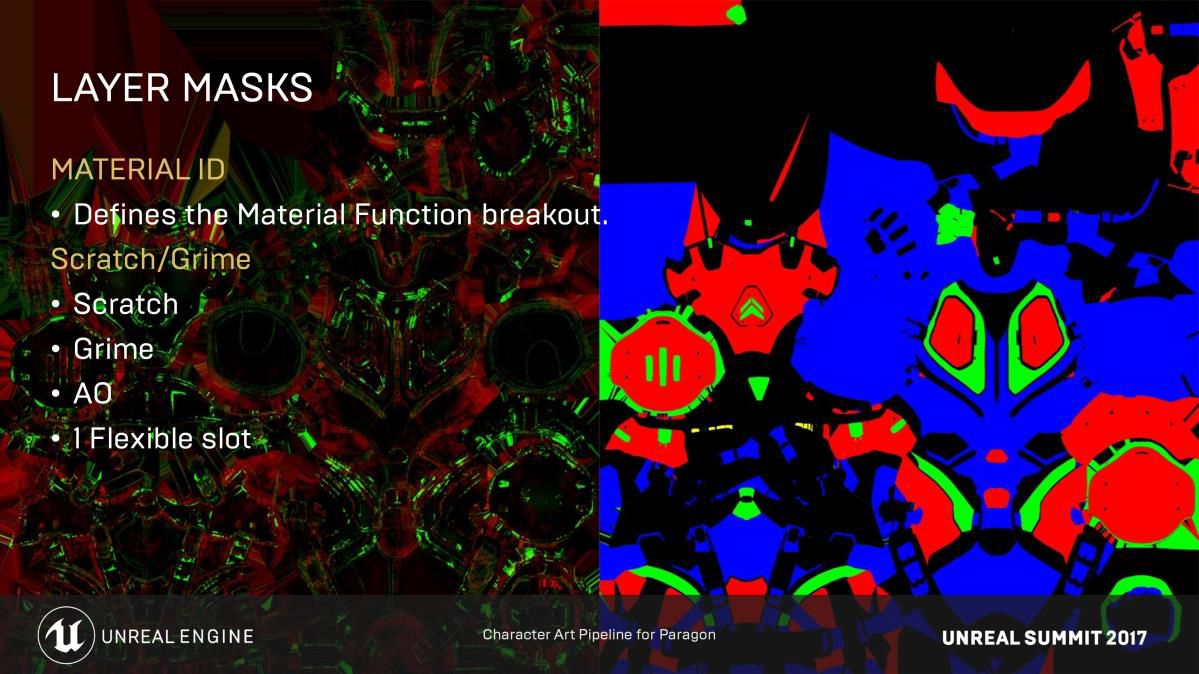
\includegraphics[width=0.7\linewidth]{images/07cha_19_ue4Presentation.jpg}
	\caption{ID maps used as layer masks for a \emph{Paragon} character. The right one defines the distinctive base materials like rubber, metal and plastic. The left contains the ambient occlusion map with additional detail masks for scratches and grime. Image source: \cite[p.\,116]{kime2017paragonsummit}.}
	\label{fig:paragonMasksSlide}
\end{figure}

\subsection{\patMaskingCreationProcedural}\label{\patMaskingCreationProcedural}
\begin{description}
	\item[\patIntent:]% 
	Use procedural methods for the dynamic and automated generation of masks. 
	%\item[\patAlsoKnownAs:]% 
	\item[\patMotivation:]% 
	You are presented a scenario of using procedural masking for exterior environment scenes in pattern \emph{\patImplementationCustomShader} (section \ref{\patImplementationCustomShader}). In that example, procedural masking is used to generate moss on top of rocks. This can be achieved by utilizing the mesh independent world space normal vector. A procedural setup that is independent from object specific data can be reused across arbitrary objects without any additional manual work. A new rock assets can be added to the scene. By assigning the proper material, it automatically uses the proper masking. Further, additional features like vertex color can be implemented to control the blending process further. Consider working on an exterior scene and in the middle of the map is a small hill. To create a smooth transition from forest ground to greenfield, you incorporate a height based masking which blends automatically between both ground base materials. 
	\item[\patApplicability:]\hfill 
	\begin{itemize}\mynobreakpar
		\item Procedural approaches can be used to create a system solving recurring problems. Instead of painting the moss on top of all rocks, you can automate the moss masking based on the world space normal.
		\item A requirement for the corresponding mask is to react to different inputs (e.g., height based base material blending).
		\item A dynamic masking system that can change at runtime (e.g., puddles reacting to a global weathering system, dynamic changes between material states, flickering emissive materials).				
	\end{itemize}
	\item[\patImplementation:]% 
	Using and controlling procedural masks requires custom shaders, \emph{\patImplementationCustomShader} (section \ref{\patImplementationCustomShader}). \emph{UE4} and \emph{Unity} provide with their shader graph editors powerful tools. They enable you to easily access different input data and utilize it to drive the procedural masking. 
	\item[\patExamples:]% 
	Figure \ref{fig:procedural mask} illustrates a layered rock shader using a procedural mask for the moss. The moss covers automatically the top of the rock. This even works by rotating the object within the 3D scene. It also works for different game objects using the same mesh and material with different rotations. The moss will always cover the top for all of them. 
	\item[\patConsequences:]\hfill 
		\begin{description}
			\item[\visual:]\hfill
			\begin{itemize}\mynobreakpar
				\item A lot of visual work is done within the shader. 
				\item Working with huge amount of different parameter inputs to control the masking might be unintuitiv. 
				\item If and to what extent the artist is able to control the masking depends on the shader. Does it enable the artist to control or influence the masking process (e.g., by utilizing vertex paint within the engine)? 
				\item This approach requires a rather abstract, logical and technical way of thinking about artistic problems. 
			\end{itemize}
			\item[\performance:]\hfill
			\begin{itemize}\mynobreakpar
				\item These masking instructions are calculated at runtime. The performance depends highly on the amount and complexity of these procedural systems.
				\item As they are less reliant on stored data, they generally use less memory than textures.
			\end{itemize}
			\item[\pipeline:]\hfill
			\begin{itemize}\mynobreakpar
				\item The shading pipeline has to support custom shaders.
				\item Masks can be reused across different assets and projects.
				\item It includes all the advantages and disadvantages of a procedural workflow. 
			\end{itemize}
		\end{description}
	\item[\patRelations:]% 
	To use flexible procedural masking, custom shader solutions are required as explained in pattern \emph{\patImplementationCustomShader} (section \ref{\patImplementationCustomShader}). This pattern is often used in addition with pattern \emph{\patWorkflowIndividualShader} (section \ref{\patWorkflowIndividualShader}). Using individual shaders enables to create problem specific procedural masks. An easy way to include procedural masking is by using pre-existing content generated shaders as in  \emph{\patWorkflowContentDrivenShader} (section \ref{\patWorkflowContentDrivenShader}). Procedural processes are to a large extent defined by the inputs. Patterns within the category \emph{\patCatExternalInputs}, section \ref{\patCatExternalInputs}, will be helpful in designing procedural masks. 
\end{description}


\begin{figure}
	\centering\small 
	\begin{tabular}{@{}cc@{}}
		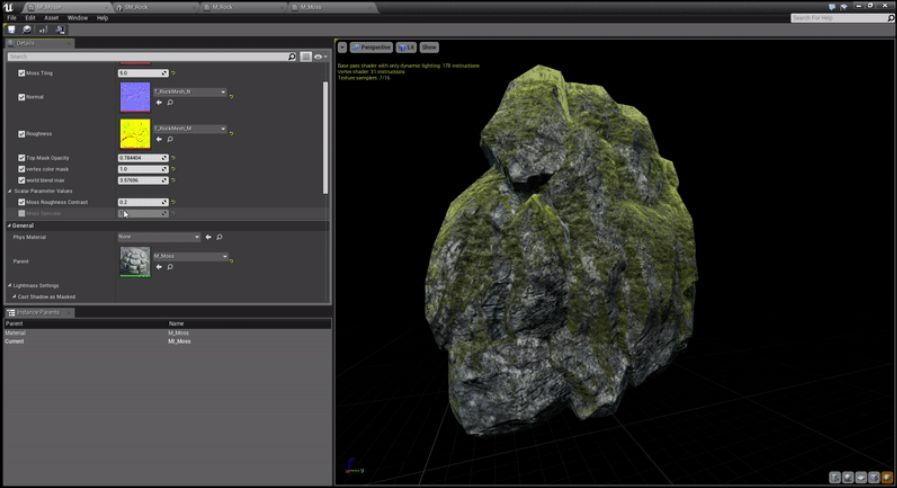
\includegraphics[width=0.475\textwidth]{images/07cha_20_mossShader(1).jpg} &
		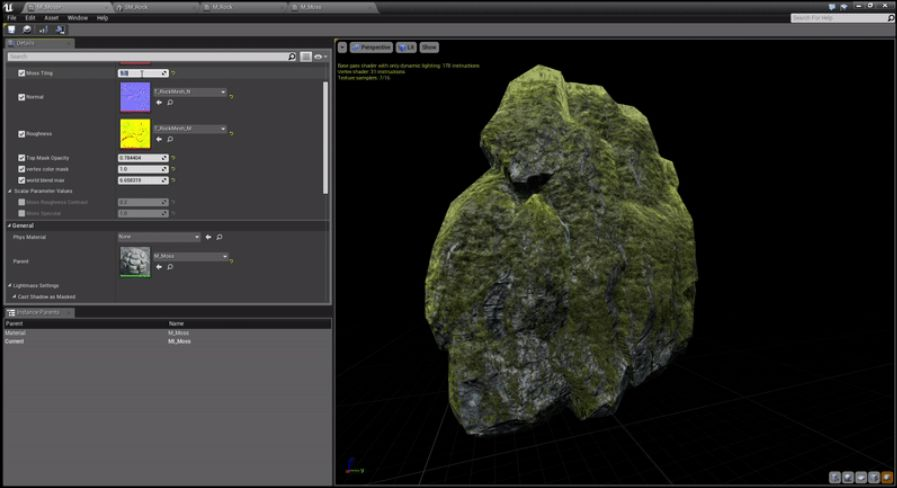
\includegraphics[width=0.475\textwidth]{images/07cha_20_mossShader(2).jpg} \\	
		(a) & (b) \\ 
	\end{tabular}
	\caption{Procedural masking of moss. A procedural shader is used to create the layer mask dynamically. The moss is blended automatically to cover the top of the rocks. Different parameters can be used to control the masking amount, direction an sharpness: less (a) and more (b) moss.
	}
	\label{fig:procedural mask}
\end{figure}



%%%%%%%%%%%%%%%%%%%%%%%%%BLENDING MODULE%%%%%%%%%%%%%%%%%%%%%%%%%%%%%%%%%%%%%%%

\section{\patCatBlendingModule}\label{\patCatBlendingModule}

The blending module is the last component of the material layering model. It inputs the material layers from the material containers and blends them based on a mask. Please refer to \ref{sec:blendingModes} for further information on this module. The following patterns, \emph{\patBlendingFull} (section \ref{\patBlendingFull}) and \emph{\patBlendingPartially} (section \ref{\patBlendingPartially}), illustrate two possible approaches for implementing such a blending module.  The pattern \emph{\patBlendingFull} (section \ref{\patBlendingFull}) represents a rather rigid system. It provides only a few blending modes. These blending modes try to be physically plausible and provide blending operations that respect the energy conservation law (except for adding emissive base materials). These blending modes define the mixing of all material parameters. Therefore, they are predictable, user friendly but limiting.  
The pattern \emph{\patBlendingPartially} (section \ref{\patBlendingPartially}), on the contrary, does not try to stay physically plausible but enables the user to blend the different parameters of the material layers individually. The user defines exactly which material parameters are skipped, blended and how they are blended. This enables the use of material layers that describe the surface only partially, see pattern \emph{\patComplexitMaterialModulation} (section \ref{\patComplexitMaterialModulation}). This allows more flexibility in how to use the resources and thus makes the use of additional layers possible. The advantage as well as disadvantage for the user is the higher control and responsibility to weigh up performance versus accuracy and artistic freedom.  

\subsection{\patBlendingFull}\label{\patBlendingFull}
\begin{description}
	\item[\patIntent:]% 
	It uses a closed an rigid blending module that is limited to only a few modes. These blending modes are designed to be physically plausible and and user friendly, producing predictable and consistent results.
	%\item[\patAlsoKnownAs:]% 
	\item[\patMotivation:]% 
	Probably the easiest way to achieve realistic looking results is by imitating real world behavior. Constraining the blending modes makes it easier to ensure a proper blending (e.g., maintain the energy conservation law). 
	\item[\patApplicability:]\hfill 
	\begin{itemize}\mynobreakpar
		\item This approach creates predictable and consistent results.
		\item Inputs are most probably mainly texture based. 
		\item The goal is to use a physically plausible system. 
	\end{itemize}
	\item[\patImplementation:]% 
	This design of the blending module can be used for all implementations. Almost any general purpose shader, see pattern \emph{\patWorkflowUberShader} (section \ref{\patWorkflowUberShader}), uses a blending module based on this design as it is flexible enough to represent all kinds of base materials and does provide a good usability. It works best with base materials using \emph{\patComplexityFulMaterial} (section \ref{\patComplexityFulMaterial}). Other shaders using pattern \emph{\patComplexitMaterialModulation} (section \ref{\patComplexitMaterialModulation}) do not work well for this concept.
	\item[\patExamples:]% 
	Figure \ref{fig:mapparFullMaterial} shows an asset from \emph{Letzte Worte}. The material is composed of different fully described base materials. These base materials are reused across different assets in this location.
	\item[\patConsequences:]\hfill 
		\begin{description}
			\item[\visual:]\hfill
			\begin{itemize}\mynobreakpar
				\item Using this physically plausable blending approach creates predictable and consistent results. Therefore, it is easy to work with. 
				\item The artistic process can focus mainly on creating appropriate base materials and the corresponding masks.
				\item It enables the artist to test different ideas and concepts out as materials can easily be changed.  
			\end{itemize}
			\item[\performance:]\hfill
			\begin{itemize}\mynobreakpar
				\item Every base material uses a full material properties description (see pattern \emph{\patComplexityFulMaterial} (section \ref{\patComplexityFulMaterial})) 
				\item The performance cost is predictable as all the different options are limited. 
			\end{itemize}
			\item[\pipeline:]\hfill
			\begin{itemize}\mynobreakpar
				\item The workflow is straight forward. The energy can be spent on creating base materials and masks. 
				\item Base material complexity and definition stay consistent throughout the project. 
			\end{itemize}
		\end{description}
	\item[\patRelations:]% 
	The blending mode is highly connected with the complexity of the base materials. This approach will not work for base materials only defined partially, see  \emph{\patComplexitMaterialModulation} (section \ref{\patComplexitMaterialModulation}).
\end{description}



\begin{figure}
	\centering
	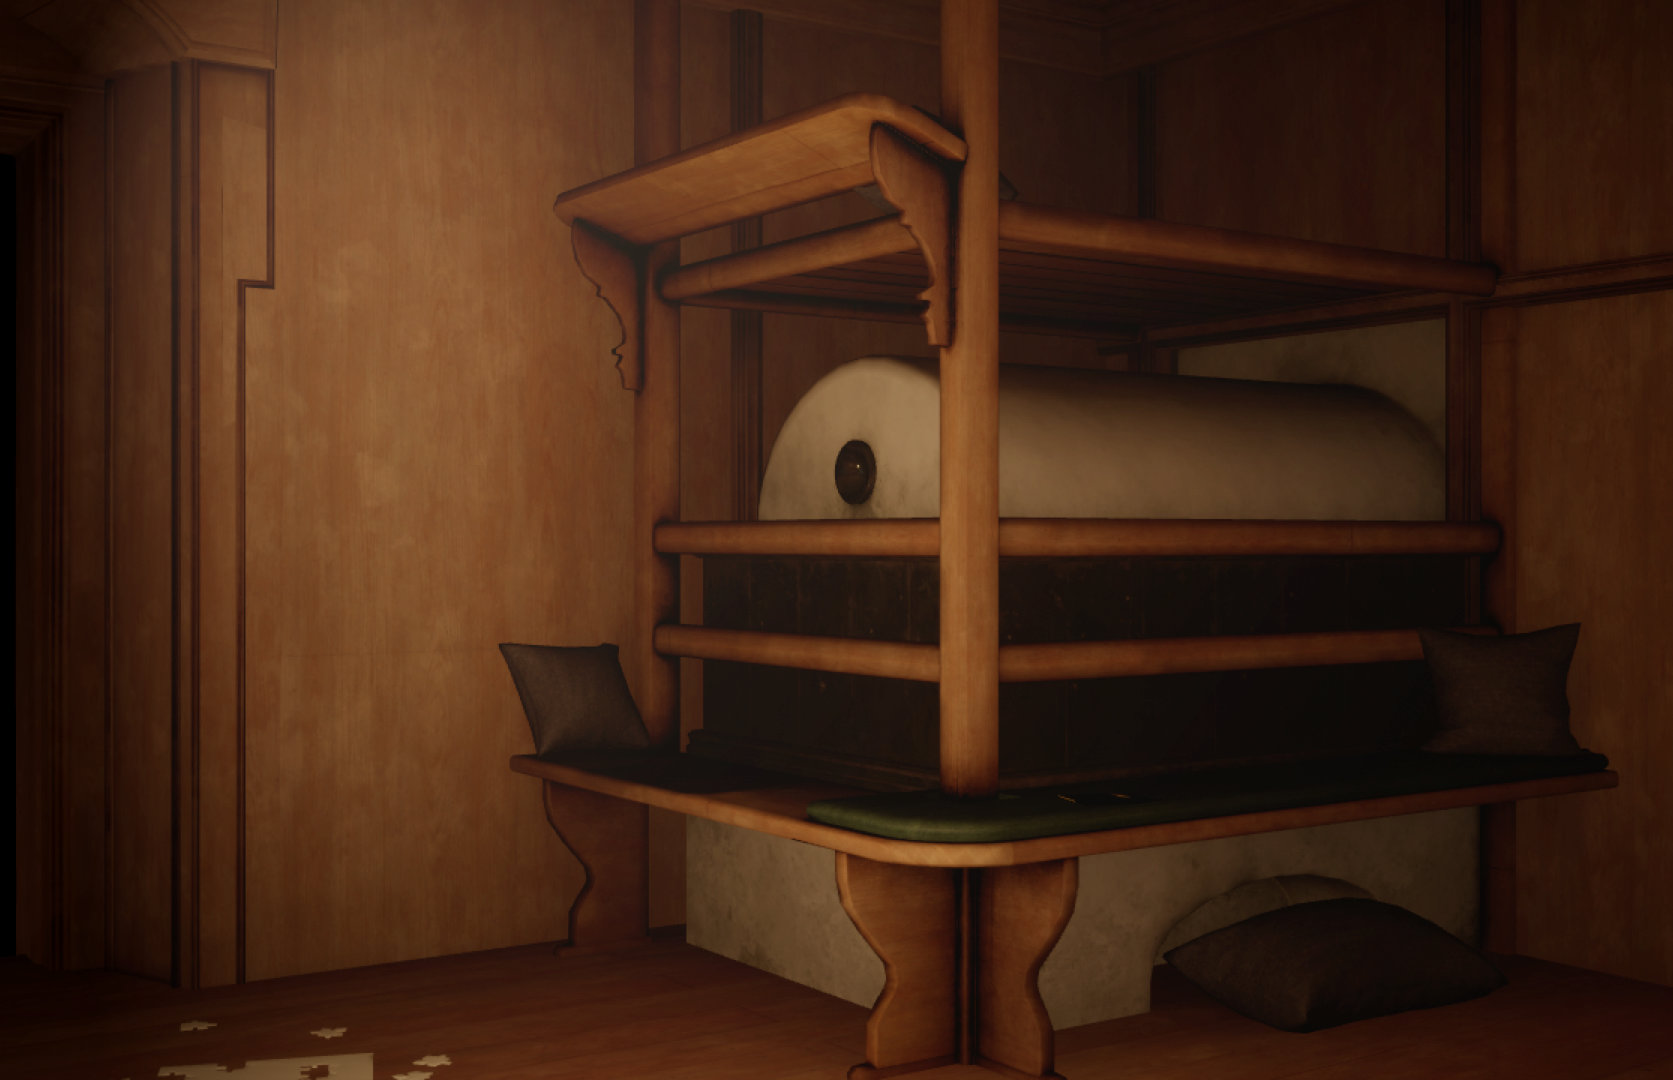
\includegraphics[width=0.7\linewidth]{images/07cha_21_MAP_par.jpg}
	\caption{An asset blending fully described base materials. 
		This image shows an early asset from \emph{Letzte Worte}. All base materials use a full material description (e.g., base color, metalness, roughness, ambient occlusion): wood, dirt, dust, fabric, used fabric, fine plastered wall and rough plastered wall. }
	\label{fig:mapparFullMaterial}
\end{figure}

\subsection{\patBlendingPartially}\label{\patBlendingPartially}
\begin{description}
	\item[\patIntent:]% 
	This blending module design is much more open and provides the possibility to define exactly which, if and how individual material parameters are blended. It does not follow the constraints of trying to be physically plausible. This flexibility allows to define more precisely how resources are used and where to sacrifice accuracy for performance.
	%\item[\patAlsoKnownAs:]% 
	\item[\patMotivation:]% 
	Consider working on a complex layered material with a huge amount of different surface types. Consider a brick wall that is partially plastered. Both base materials use the pattern \emph{\patComplexityFulMaterial} (section \ref{\patComplexityFulMaterial}) and are described in all their properties. Additional layers are introduced to add variety. For the plastered wall they are as follows: a water damaged variation, ground dirt, a newly plastered part and a slightly damaged variety. For the brick the following variations are added: a color variation and a water damaged version. Considering three textures per base material results in eight base materials using twenty-four textures. If we use only the base color texture for each variation and simply subtract or add a small scalar to the roughness value depending on the variation, the texture count gets divided by half. The result might not be physically accurate but it pays off as far as performance increase: a lower amount of used texture memory and computation instructions.
	\item[\patApplicability:]\hfill
	\begin{itemize}\mynobreakpar
		\item This approach is well suited for large amounts of similar base materials.
		\item It works well if only a single  material property is replaced.
		\item Custom material blending works great creating surface variation, e.g., puddles and water. Wetness can easily be achieved by manipulating the normal map, darkening the base color and decreasing the roughness. 
	\end{itemize}
	\item[\patImplementation:]% 
	To achieve this high control over how to blend which individual material parameter, it is necessary to use custom shading solutions, \emph{\patImplementationCustomShader} (section \ref{\patImplementationCustomShader}). Generally, this will require  \emph{\patWorkflowIndividualShader} (section \ref{\patWorkflowIndividualShader}) as this provides most flexibility.  Using \emph{\patWorkflowContentDrivenShader} (section \ref{\patWorkflowContentDrivenShader}) is the easiest way to incorporate this aspect into your pipeline.
	\item[\patExamples:]% 
	Figure \ref{fig:leafloorwaterblend} shows a small example for this design pattern. Using pattern \emph{\patBlendingFull} (section \ref{\patBlendingFull}) would result in either the need to create a duplicate base material representing the floor wood surface covered with water or need to to create an arbitrary blend mode that can combine an arbitrary transparent base material stacked on top of another. The former is unflexible as a wet material variation for any base materials needs to be created. The latter is technically challenging and has probably a huge impact on performance (see section \ref{sec:illuminationLobeLayering} in chapter \ref{cha:materialLayering}).
	\item[\patConsequences:]\hfill 
		\begin{description}
		\item[\visual:]\hfill
			\begin{itemize}\mynobreakpar
				\item It enables the combination of a great number of different base materials.
				\item Blending is based on visual appearance rather than any physical plausibility. 
			\end{itemize}
			\item[\performance:]\hfill
			\begin{itemize}\mynobreakpar
				\item Reducing base material and blending complexity affects performance positively. 
			\end{itemize}
			\item[\pipeline:]\hfill
			\begin{itemize}\mynobreakpar
				\item The pipeline needs to provide more control over if and how individual material parameters get blended. 
				\item The best way to incorporate this pattern into your project is by using \emph{\patWorkflowContentDrivenShader} (section \ref{\patWorkflowContentDrivenShader}).
			\end{itemize}
		\end{description}
	\item[\patRelations:]%
	This approach works, in contrast to the previous \emph{\patBlendingFull} (section \ref{\patBlendingFull}), with all base materials well, both using \emph{\patComplexityFulMaterial} (section \ref{\patComplexityFulMaterial}) and \emph{\patComplexitMaterialModulation} (section \ref{\patComplexitMaterialModulation}). 
\end{description}

\begin{figure}
	\centering
	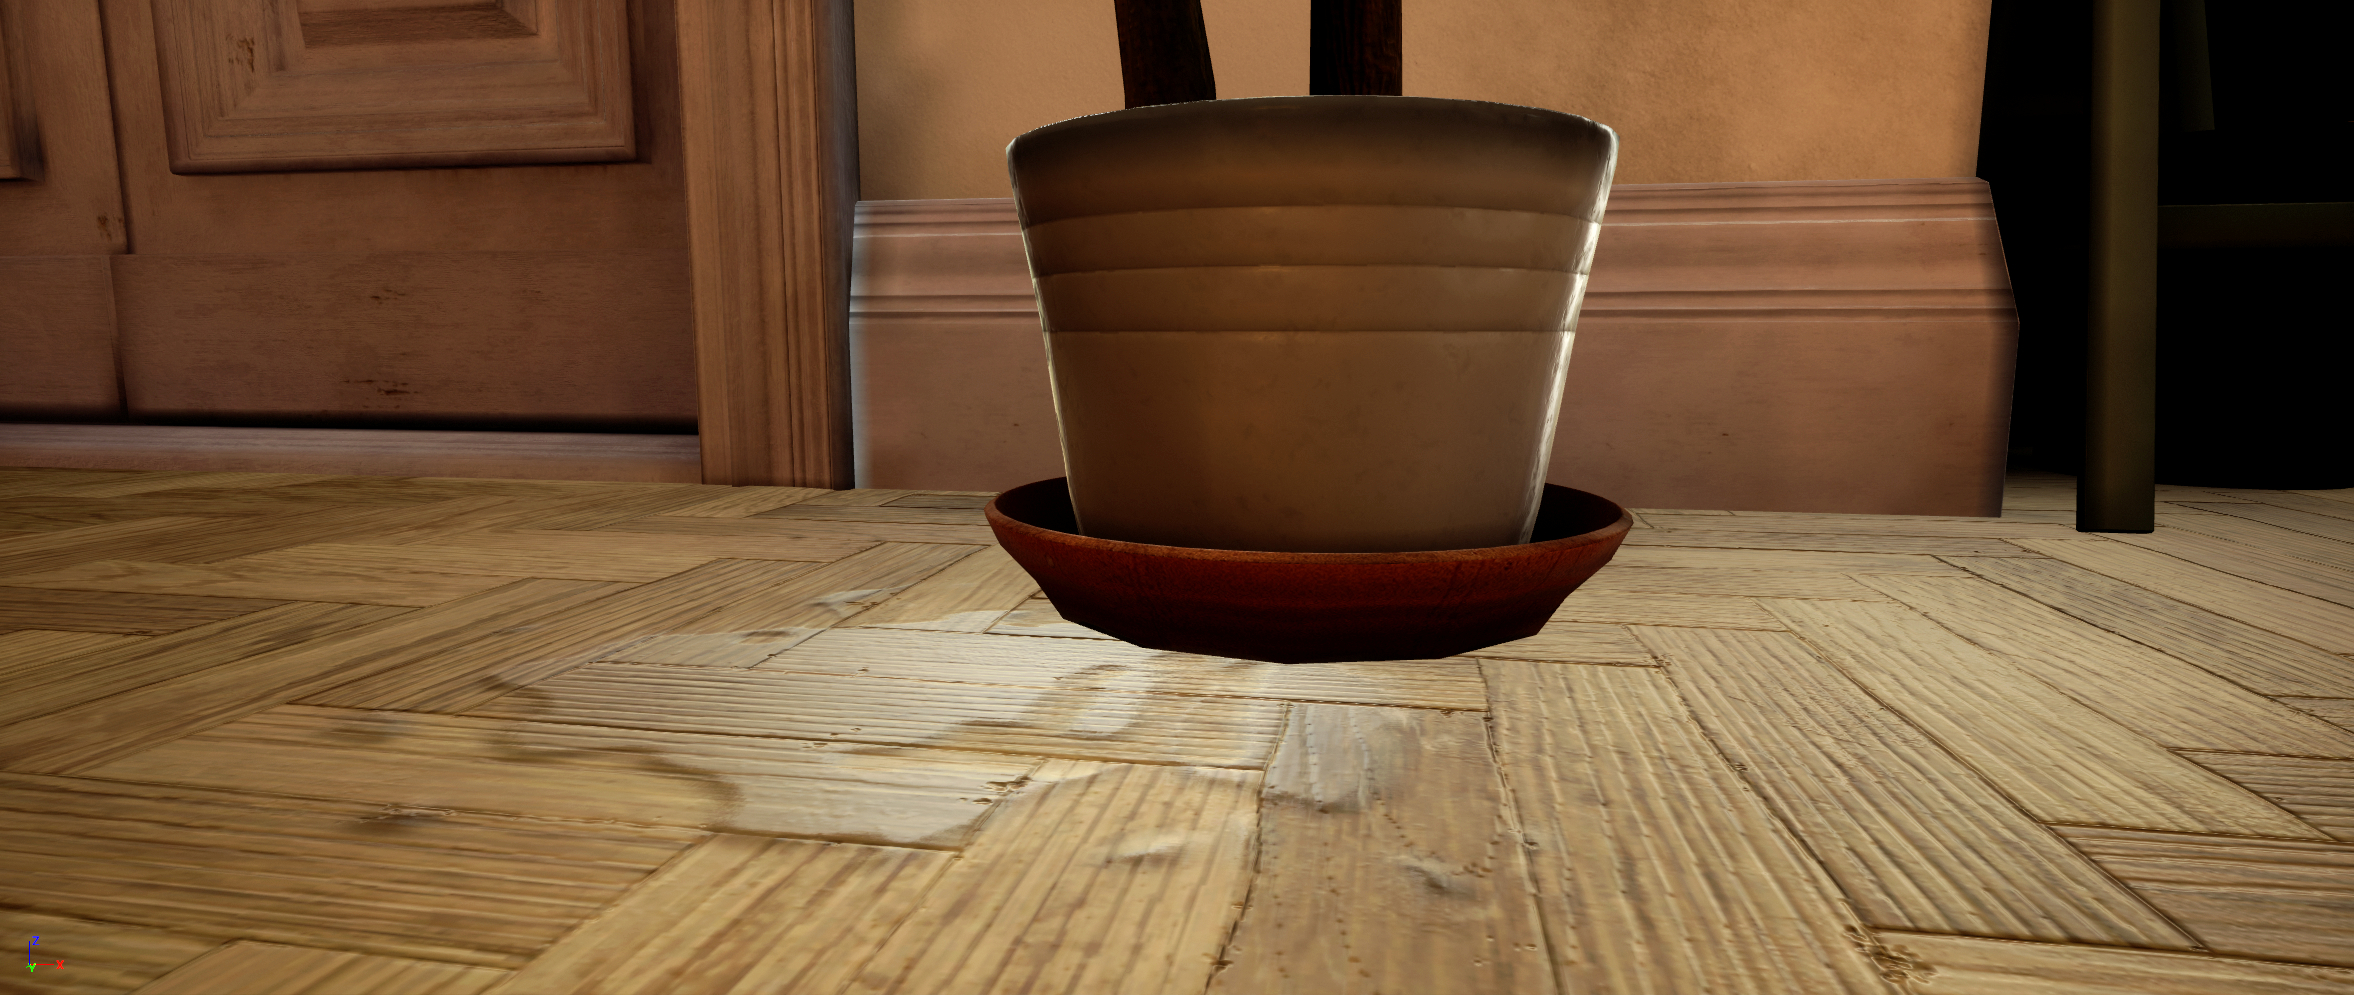
\includegraphics[width=0.7\linewidth]{images/07cha_22_leaFloorWaterBlend.jpg}
	\caption{\NEW
		The water material layer is not described by all material properties. The appearance of water on top of a surface is created by using custom blending of individual properties.   }
	\label{fig:leafloorwaterblend}
\end{figure}
%(\emph{\patBlendingPartially} in \ref{\patBlendingPartially})



%%%%%%%%%%%%%%%%%%%%%%%%%EXTERNAL INPUTS PARAMETERS%%%%%%%%%%%%%%%%%%%%%%%%%%%%%%%%%%%%%%%

\section{\patCatExternalInputs}\label{\patCatExternalInputs}

This category presents different patterns associated with utilizing different external inputs. In this case, external refers to data that is not embedded within the shader, like parameters, mesh data, object data and scene data. These different inputs with their distinctive advantanges and disadvantages will be discussed in the following categories. 


%\begin{patternCategory02}
%	{orange} %color	
%	{\patCatParameters} %header
%\end{patternCategory02}\label{\patCatParameters}
\subsection{\patCatParameters}\label{\patCatParameters}

This category includes basically all parameters that can be exposed by the shader to be set in the material (e.g., textures, vector and scalar paremeters). The following patterns present different use cases for this kind of inputs. As textures play such a fundamental role in shading, the design pattern \emph{\parParametersTextures} (section \ref{\parParametersTextures}) focuses entirely on them. \emph{\parParametersVariables} (section \ref{\parParametersVariables}) present other types of parameter inputs, like colors, position vectors, scalar value and switches. In pattern \emph{\parParametersScripted} (section \ref{\parParametersScripted}), I want to illustrate possibilities to utilize scripted parameters.

\subsubsection{\parParametersTextures}\label{\parParametersTextures} %TODO examples
\begin{description}
	\item[\patIntent:]% 
	Use textures as a data table to define different material properties, masks or as input for procedural operations.   
	%\item[\patAlsoKnownAs:]% 
	\item[\patMotivation:]% 
	Consider a project that targets a photorealistic art style. Textures are ideal as they are perfect to store complex surface information of all kinds. Furthermore, a wide variety of processes to generate textures exist (e.g., 3D scanning, photo editing, baking of procedural or high detailed 3D data and painting). Specialized texture tools make it quite easy to generate realistic looking textures.
	\item[\patApplicability:]\hfill
	\begin{itemize}\mynobreakpar
		\item Complex surface information can be stored within textures easily.
		\item Huge libraries of high quality textures exist and can be utilized for the current project. 
		\item Textures can be baked down from procedural approaches, vertex color or different 3D data. 
		\item Textures can be used to store arbitrary data.
		\item A lot of applications are especially designed to generate, create and paint textures.  
		%\item Textures can easily be shared across different applications. 
		\item Artists are used to working with textures. It is a familiar workflow. 
		\item Commercial engines like \emph{UE4} and \emph{Unity} have already been well optimized for working with a large number of bigger textures. They use technologies like mid-mapping, texture streaming and advanced compressions. 
		\item Textures are set per material. All assets using the same material share the same textures. 
	\end{itemize} 
	\item[\patImplementation:]% 
	A wide variety of different tools and approaches exist to create and generate textures. Textures can be created of photos, 3D scans or by using procedural methods.
	%\item[\patExamples:]% 
	\item[\patConsequences:]\hfill 
		\begin{description}
			\item[\visual:]\hfill
			\begin{itemize}\mynobreakpar
				\item Complex surface data can easily be created and stored.
				\item Textures generally provide the most efficient way to store huge surface data. 
				\item Artists are used to working with textures. A lot of tools make working with textures intuitive. 
				\item A lot of tools exist to generate, create and paint textures.
				\item Textures are projected onto objects. This projection can be manipulated to rotate, offset and scale textures. Textures can even be animated by manipulating these projection coordinates. 
			\end{itemize}
			\item[\performance:]\hfill
			\begin{itemize}\mynobreakpar
				\item Textures have already been highly optimized through technologies like texture streaming, compression, mid-maping, filtering.
				\item Huge textures need a large amount of memory. 
				\item The loading of large textures into the VRAM may take some time. 
				\item The streaming of texture data has a huge impact on loading times.   
				\item Methods like combining different objects into texture atlases and channel packing reduce the amount of textures.  
			\end{itemize}
			\item[\pipeline:]\hfill
			\begin{itemize}\mynobreakpar
				\item Textures can easily be created in other applications.
				\item Texture data is easy to share between different softwares.
				\item They can be stored in libraries and easily be modified and reused.
			\end{itemize}
		\end{description}
	\item[\patRelations:]% 
	Textures are used across all different pattern layering implementations and workflows. They are used within material containers to define base material properties directly or as an additional input to drive and manipulate procedural methods. They play an vital role in creating mask. 
\end{description}


\subsubsection{\parParametersVariables}\label{\parParametersVariables}
\begin{description}
	\item[\patIntent:]% 
	Variables can be set per material or per component on advanced material layering systems. The most common parameters are textures, vectors, scalar values, booleans and switches.
	%\item[\patAlsoKnownAs:]% 
	\item[\patMotivation:]% 
	You want to specify different colors for different materials using the same shader. To do so, expose a color vector within the shader. This parameter can later be specified in the materials panel of the individual material. In another example, a procedural masking container uses the world position normals to mask areas facing the top. To add more control, you can expose an additional vector that enables you to influence the direction to be masked. In one material you want to influence the opacity of an individual material layer. Therefore, you add a scalar parameter to the shader and multiply it with the blend opacity of the material layer. Within the material you can now influence the material layer blend opacity.
	\item[\patApplicability:]\hfill
	\begin{itemize}\mynobreakpar
		\item You wish to influence colors, vectors, opacities, switches and features on a per material basis. 
		\item You expose parameters to control procedural processes.
		\item You want to tweak values in engine (e.g., adjust the roughness value slightly).
	\end{itemize}
	\item[\patImplementation:]%
		In a \emph{\patImplementationCustomShader} (section \ref{\patImplementationCustomShader}) you can simply define which parameters should be exposed to be set in the individual materials. In a  \emph{\patImplementationBUildtIn} (section \ref{\patImplementationBUildtIn}) all available parameters are defined by the shader and can not be changed. 
	%\item[\patExamples:]% 
	%\item[\patConsequences:]\hfill \begin{description}
	\item[\patRelations:]% 
	Custom parameters can easily be exposed within a \emph{\patImplementationCustomShader} (section \ref{\patImplementationCustomShader})
\end{description}


\subsubsection{\parParametersScripted}\label{\parParametersScripted}

\begin{description}
	\item[\patIntent:]% 
	Scripted parameters are regular material parameters accessed from within the game code to either set or change them at runtime. 
	%\item[\patAlsoKnownAs:]% 
	\item[\patMotivation:]% 
	Imagine a flickering light bulb. You could either create the flickering by using procedural noises within the shader or by controlling certain parameters, like emissive color or intensity, from a script. 	
	\item[\patApplicability:]\hfill
	\begin{itemize}\mynobreakpar
		\item Surface properties are supposed to change at runtime.
		\item The game logic should influence certain material properties. 
		\item You want to access additional information that cannot be accessed from within the shader graph editor. Therefore, you want the game logic to set a property within the material, e.g., you can pass on the position vector of an arbitrary object within your scene to the shader using a vector parameter.
	\end{itemize}
	\item[\patImplementation:]% 
	\emph{UE4} provides an artist friendly visual coding environment, the \emph{Blueprints Visual Scripting} system. You can utilize this scripting environment to set and manipulate parameters within your materials. 
	%\item[\patExamples:]% 
	%\item[\patConsequences:]\hfill \begin{description}
	\item[\patRelations:]% 
	This pattern uses regular parameter values \emph{\parParametersVariables} (section \ref{\parParametersVariables}) that are set or manipulated at runtime by the game code. 
\end{description}


\begin{figure}
	\centering
	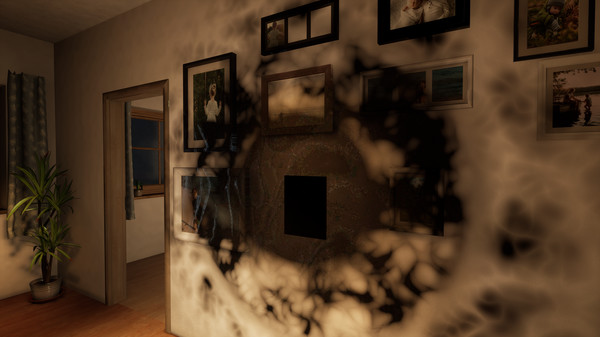
\includegraphics[width=0.7\linewidth]{images/07cha_23_expansionDarnkess.jpg}
	\caption{A Layered Material from \emph{Letzte Worte} using scripted parameters. This shader reacts to the player action. When triggered, the dark area grows to cover a big portion of the wall. The parameters to control this expansion are set and animated from the game code.}
	\label{fig:expansiondarnkess}
\end{figure}


%%%%%%%%%%%%%%%%%%%%%%%%%EXTERNAL INPUTS MASH DATA%%%%%%%%%%%%%%%%%%%%%%%%%%%%%%%%%%%%%%%

\subsection{\patCatMeshData}\label{\patCatMeshData}

The results of the previously mentioned input methods are applied globally to all meshes using the same material. Changes in the input parameters, like changing an id map for example, will inevitable effect all objects using this material instance. The inputs within this category are only influenced by the mesh data (e.g., UV coordinates, object-space normals and object space position). These inputs will be constant across all objects using the same mesh. \emph{\patMeshDataUVs} (section \ref{\patMeshDataUVs}) %,\emph{\patMeshDataVectors} on page \pageref{\patMeshDataVectors} 
and \emph{\patMeshVertexColor} (section \ref{\patMeshVertexColor}) show different methods to utilize these mesh specific properties within the shading process. This kind of parameter can be used to create variety across objects using the same material.  

\subsubsection{\patMeshDataUVs}\label{\patMeshDataUVs}
\begin{description}
	\item[\patIntent:]% 
	Use the UV coordinates to influence, manipulate and animate the projection of textures onto the object. 
	%\item[\patAlsoKnownAs:]% 
	\item[\patMotivation:]% 
	You want to add ornamental panels and trims to your scene. The intent is to combine them with pattern layering. The ornamental data for the panels and trims is sculpted within \emph{zBrush} and finally baked down to a texture. The first UV set is set out nicely and does not have any overlapping areas. All UV islands stay within the UV boundaries. This first UV set is used for the tileable base materials as well as the object specific textures. The second one is arranged more freely to project the ornamental parts onto different areas of the mesh. This second UV map does not need to be set out as cleanly as the first (e.g., inconsistent texel density, overlapping areas and UV islands exceeding the UV boundaries). It is neither used to texture the entire object nor to generate the lightmap. You can duplicate this object and use the second UV map to project different details onto the copy. This allows to create variations by using the same materials in the engine. The mapping is changed by the UV set. As the first UV map is the same, object specific texture data can still be shared across these objects.
	\item[\patApplicability:]\hfill 
	\begin{itemize}\mynobreakpar
		\item It is used for adding detail that is independent from the first UV set. 
		\item The UV coordinates can be used to offset textures, for example base materials to avoid repeating textures on the same object. This can be done by either offsetting UV coordinates pseudo randomly from within the shader or by exporting different meshes from the 3D content creation application. 
		\item It can be used to blend different texture variations. Each variation is placed on a grid; offsetting the UVs by this grid will switch the material properties projected onto the object. 
		%\item UV input can be use used to animate textures. 
	\end{itemize}
	\item[\patImplementation:]%
	3D content creation software provides the functionality to add additional UV sets. These UV sets can be modified independently and sent to the game engine. It is important to ensure that the proper UV set is used to generate the lightmap, otherwise ugly artifacts may appear.   
	\item[\patExamples:]% 
	Trim sheets are an excellent example on how the UV coordinates can be used to influence shading. Figure \ref{fig:GearsTrimPattern} shows an example from \emph{Gears of War 4}.
	\item[\patConsequences:]\hfill 
		\begin{description}
			\item[\visual:]\hfill
			\begin{itemize}\mynobreakpar
				\item It provides high control where to put additional detail. 
				\item This method allows to create highly detailed areas which can be sculpted and be reused across different assets sharing the same style. 
			\end{itemize}
			\item[\performance:]\hfill
			\begin{itemize}\mynobreakpar
				\item Creating variations by offsetting UV coordinates is easy and cheap.
				\item Animations done by manipulating the UV coordinates do not require sprite sheets where every single frame is saved as a individual picture. 
				\item Using multi UV sets in connection with normal maps may cause problems. In \emph{Letzte Worte}, normal maps caused problems when using the second UV set. The normal map effect appeared inverted for certain areas on the objects. 
			\end{itemize}
			\item[\pipeline:]\hfill
			\begin{itemize}\mynobreakpar
				\item Working with multiple UV maps can be challenging.
				\item Some software does not support multiple UV sets (e.g., \emph{Substance Painter}).
				\item Engine shaders need to be re-built within the 3D content creation application to preview a similar result to the final in engine render.   
			\end{itemize}
		\end{description}
	\item[\patRelations:]% 
	Different UV coordinates can be used in any \emph{\patImplementationCustomShader}. Especially with procedural methods, it provides a powerful tool to create performance efficient variations, see \emph{\patCreationProcedural} (section \ref{\patCreationProcedural}) and \emph{\patMaskingCreationProcedural}	 (section \ref{\patMaskingCreationProcedural}).
\end{description}



\begin{figure}
	\centering\small 
	\begin{tabular}{@{}cc@{}}
		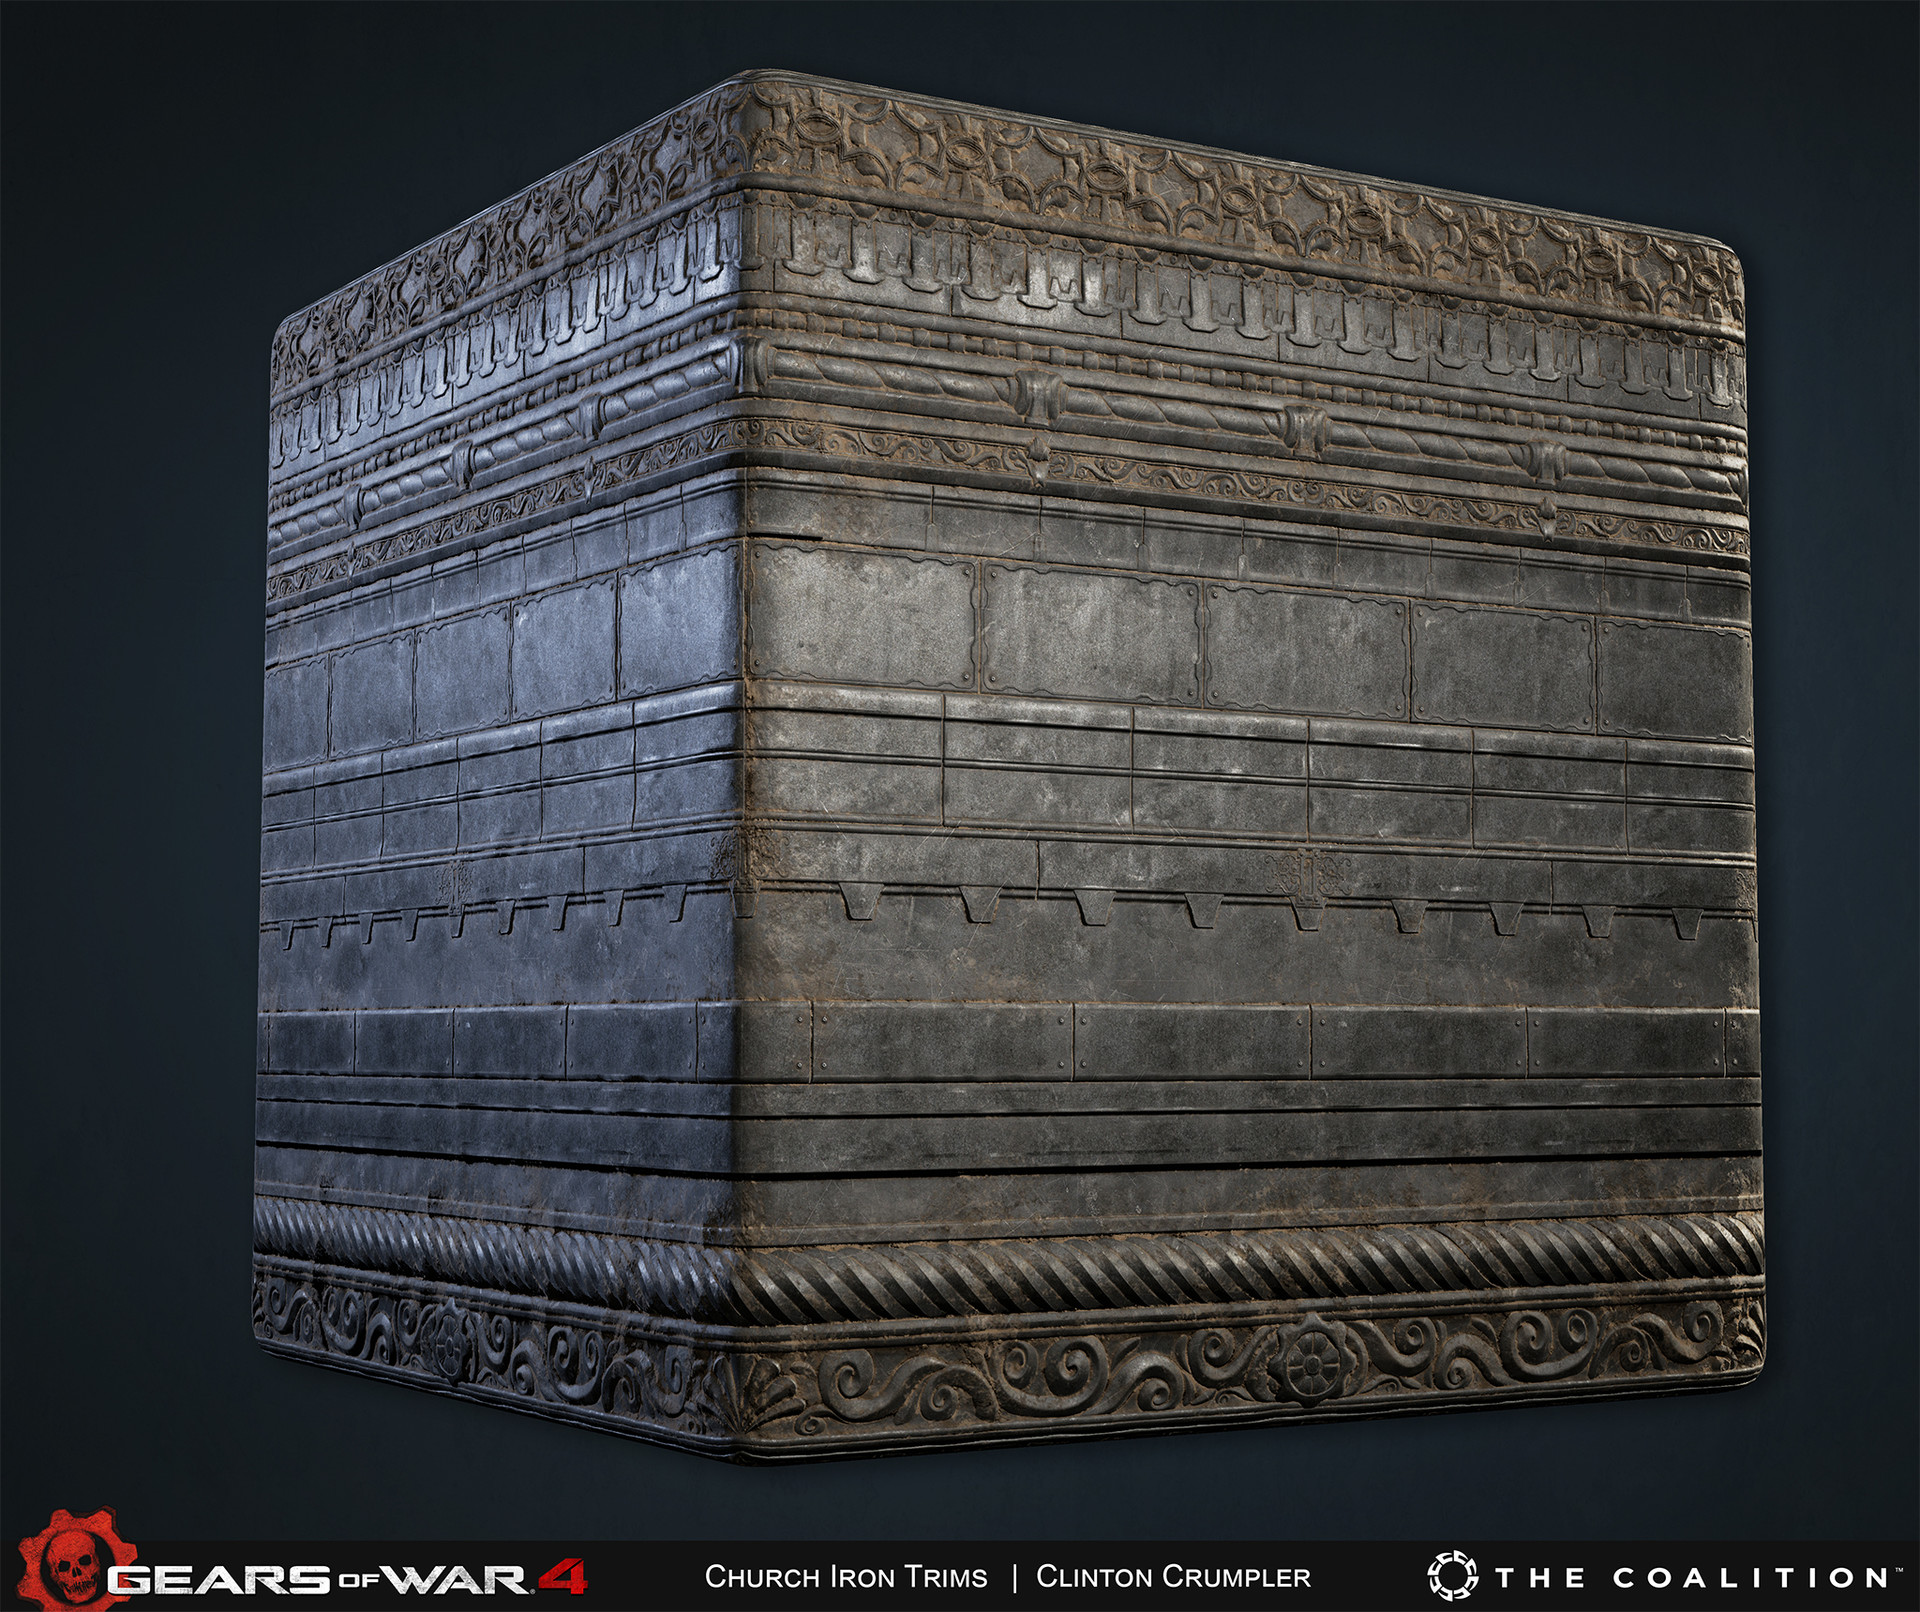
\includegraphics[width=0.25\textwidth]{images/07cha_24_clinton-crumpler-crumpler-51-copy.jpg} &
		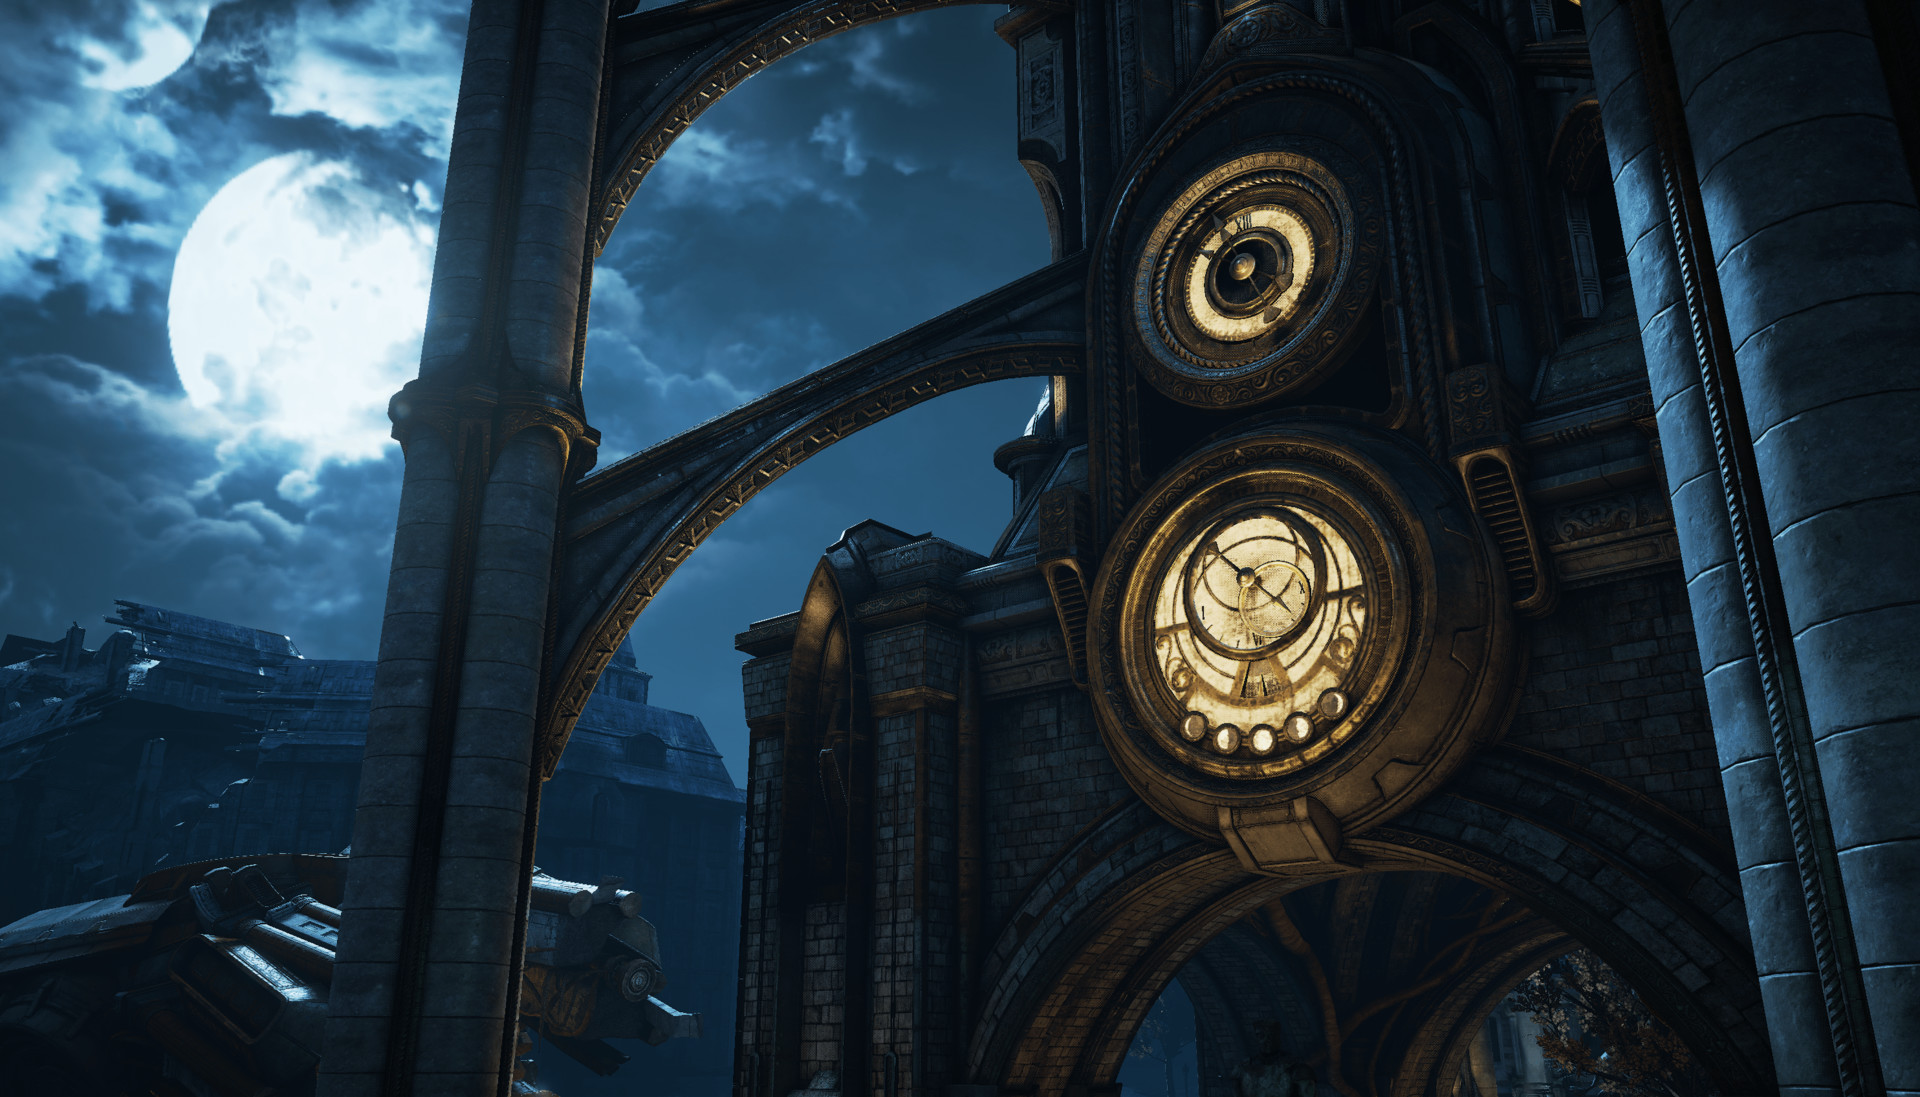
\includegraphics[width=0.65\textwidth]{images/07cha_24_clinton-crumpler-highresscreenshot00023-min.jpg} \\	
		(a) & (b)
	\end{tabular}
	
	\caption{A scene textured by combining pattern layering with trim sheets. 
		Figure (b)  shows a location from \emph{Gears of War 4} combining pattern layering with trim sheets, see figure (a). Image source: \cite{crumpler2016Gears}.}
	\label{fig:GearsTrimPattern}
\end{figure}



\subsubsection{\patMeshVertexColor}\label{\patMeshVertexColor}
\begin{description}
	\item[\patIntent:]% 
	Use vertex attributes to create per object variety independent from the material.
	%\item[\patAlsoKnownAs:]% 
	\item[\patMotivation:]% 
	Consider an often recurring object that might even be located side by side. This could be a fence, a book, a wall, a tree. Visible repeating patterns between the objects are noticeable because they use the same texture maps as a mask input for the material layering. Creating individual bitmap masks or materials is not really an option because of performance issues regarding draw calls and memory limitations. 
	This problem can be solved by using vertex attributes. The vertex attributes are independent from the material and can be different for every object. This is also true if the objects share the same mesh or material. Each vertex has a vertex color attribute that stores RGBA values. These values can be retrieved as an input parameter within the shader and be used to manipulate the material parameters. The vertex color can be used directly to color the object or indirectly, for example as a mask. The value between each color channel can be used to mask out a material.	Coloring and blending with vertex color is unique to a single object, in contrast to the id map method as mentioned before \cite{epic2018assetVsInstance}. One huge constraint of vertex color is its limitation in resolution. The vertex paint resolution is directly connected to the vertex count of the mesh. To create sharp masks, a huge vertex count is necessary. This method alone is therefore mostly used to mask out bigger areas or in connection with other methods like height warp and brush maps.
	\item[\patApplicability:]\hfill 
	\begin{itemize}\mynobreakpar
		\item The used base materials do not change between the instances. 
		\item The material blending takes place at a larger scale and not in detail space. 
	\end{itemize}
	\item[\patImplementation:]%
	The vertex color can be used as a mask to blend the different textures. This method is really powerful. The vertex shader normally implements four channels, rgba, which enables the artists to blend between five base materials. 
	\item[\patExamples:]% 
	Figure \ref{fig:vertexColor} from the \emph{Unity} project \emph{Fontainebleau} \cite{fontainebleu2018} shows how vertex color can be used to control the masking in pattern layering system.
	\item[\patConsequences:]\hfill 
		\begin{description}
			\item[\visual:]\hfill
			\begin{itemize}\mynobreakpar
				\item Vertex colors can be painted within the engine.
				\item Generally, you can paint immediately adopting the final shader. 
				\item The painting resolution depends on the geometry. Higher vertex count results in a larger painting resolution. 
				\item It works great for masking out areas but not for painting really detailed small scale areas. 
				\item Additionally, other techniques can be used to create more detailed textures (e.g., height warp, brush maps).
			\end{itemize}
			%			\item[\performance:]\hfill
			%			\begin{itemize}\mynobreakpar
			%				\item 
			%			\end{itemize}
			\item[\pipeline:]\hfill
			\begin{itemize}\mynobreakpar
				\item Some engines do already provide vertex painting tools built-in, e.g., \emph{UE4}.
				\item The masking takes place in the engine with the final shader. 
				\item Vertex color can either be imported from the 3D content creation application or be overwritten from within the engine. By overwriting it in engine, re-importing changed mesh data, may destroy the painted masks.  
			\end{itemize}
		\end{description}
	%\item[\patRelations:]% 
\end{description}


\begin{figure}
	\centering\small 
	\begin{tabular}{@{}cc@{}} % mittlerer Abstand = 12mm
		\multicolumn{2}{c}{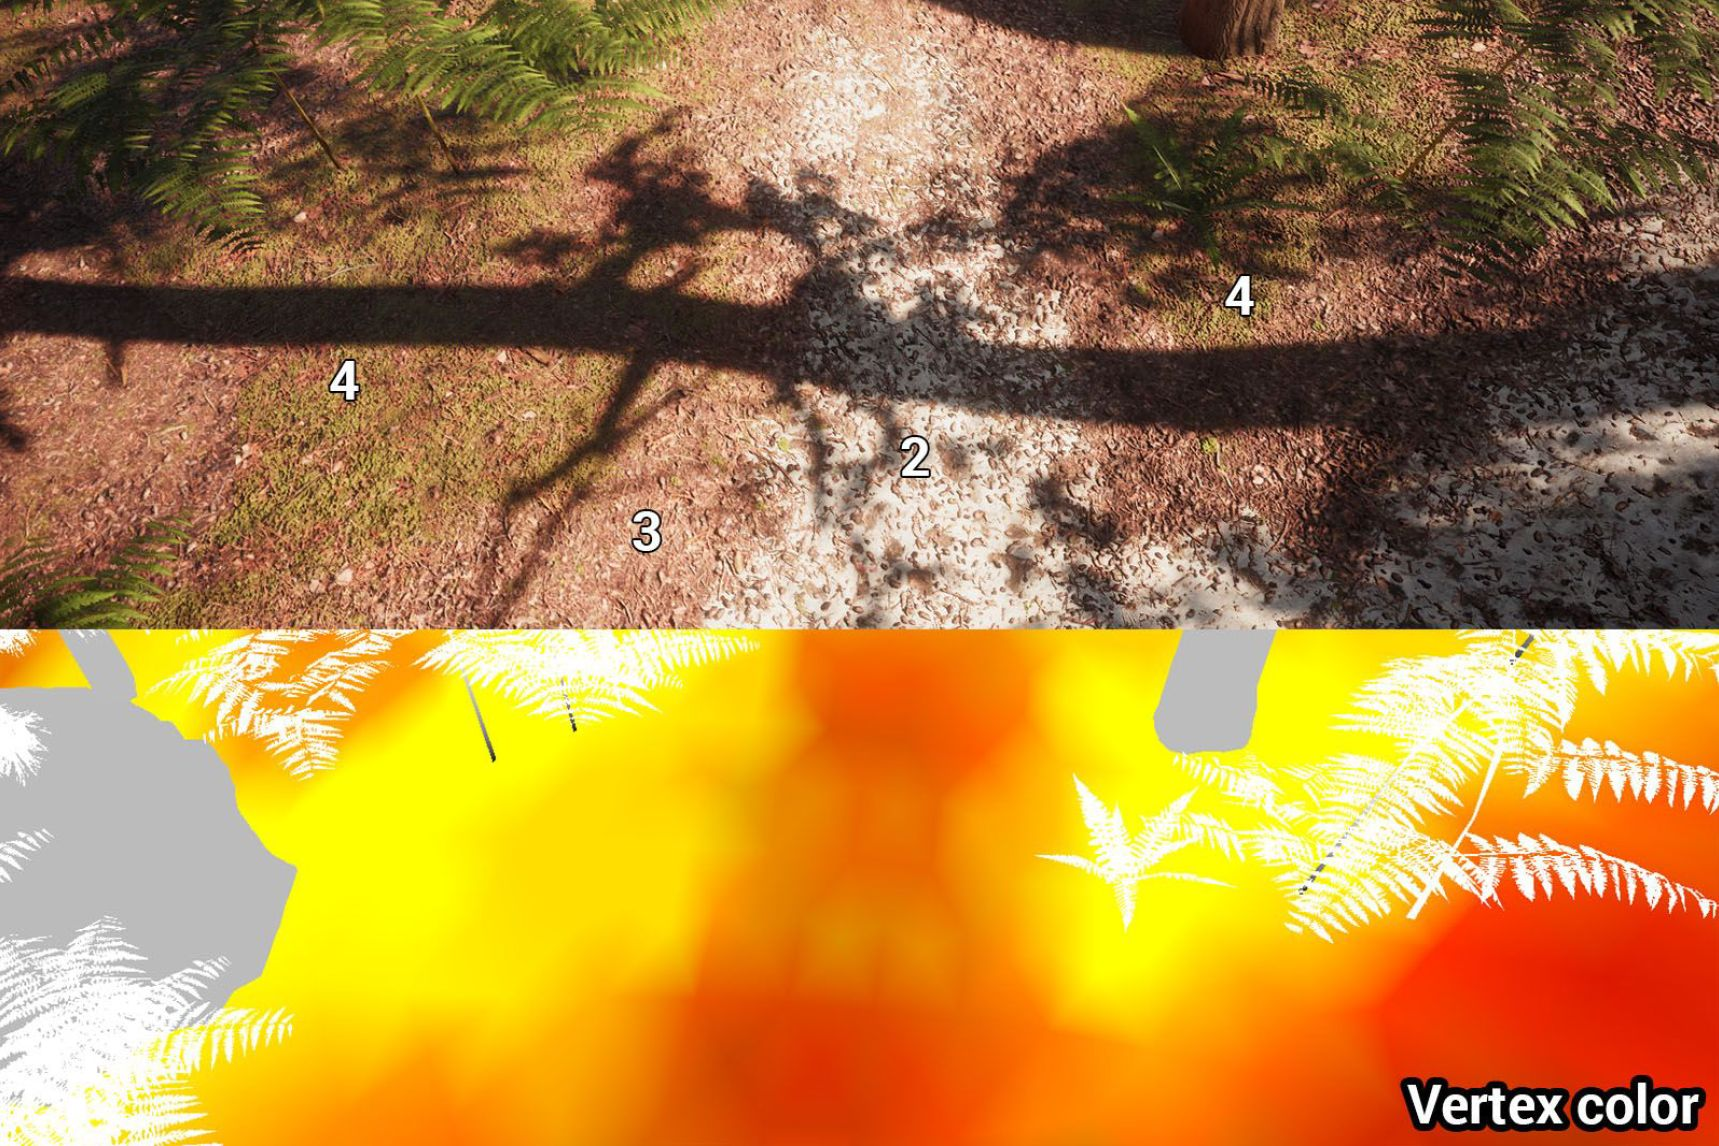
\includegraphics[width=0.75\textwidth]{images/07cha_25_layeredLitUnity_vertex01.jpg}} \\
		\multicolumn{2}{c}{(a)} \\[6pt]	%vertical extra spacing (4 points)
		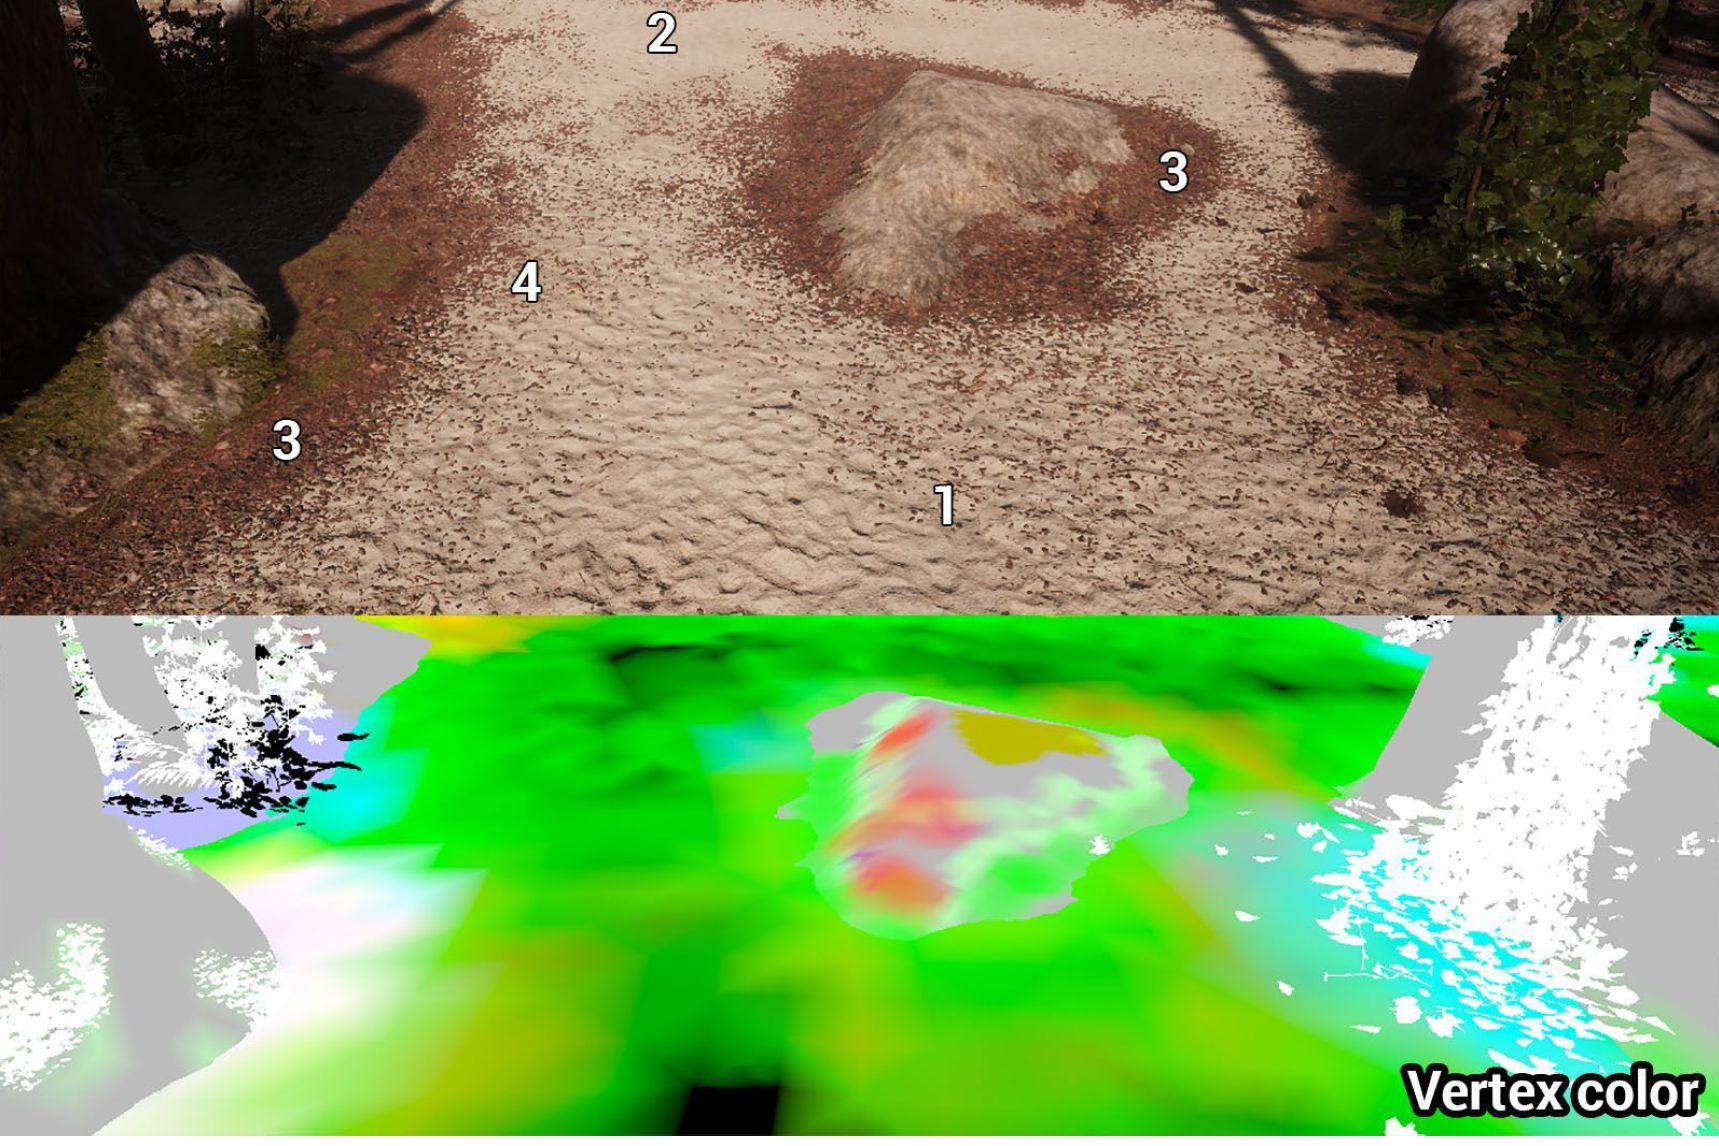
\includegraphics[width=.475\textwidth]{images/07cha_25_layeredLitUnity_vertex02.jpg} &
		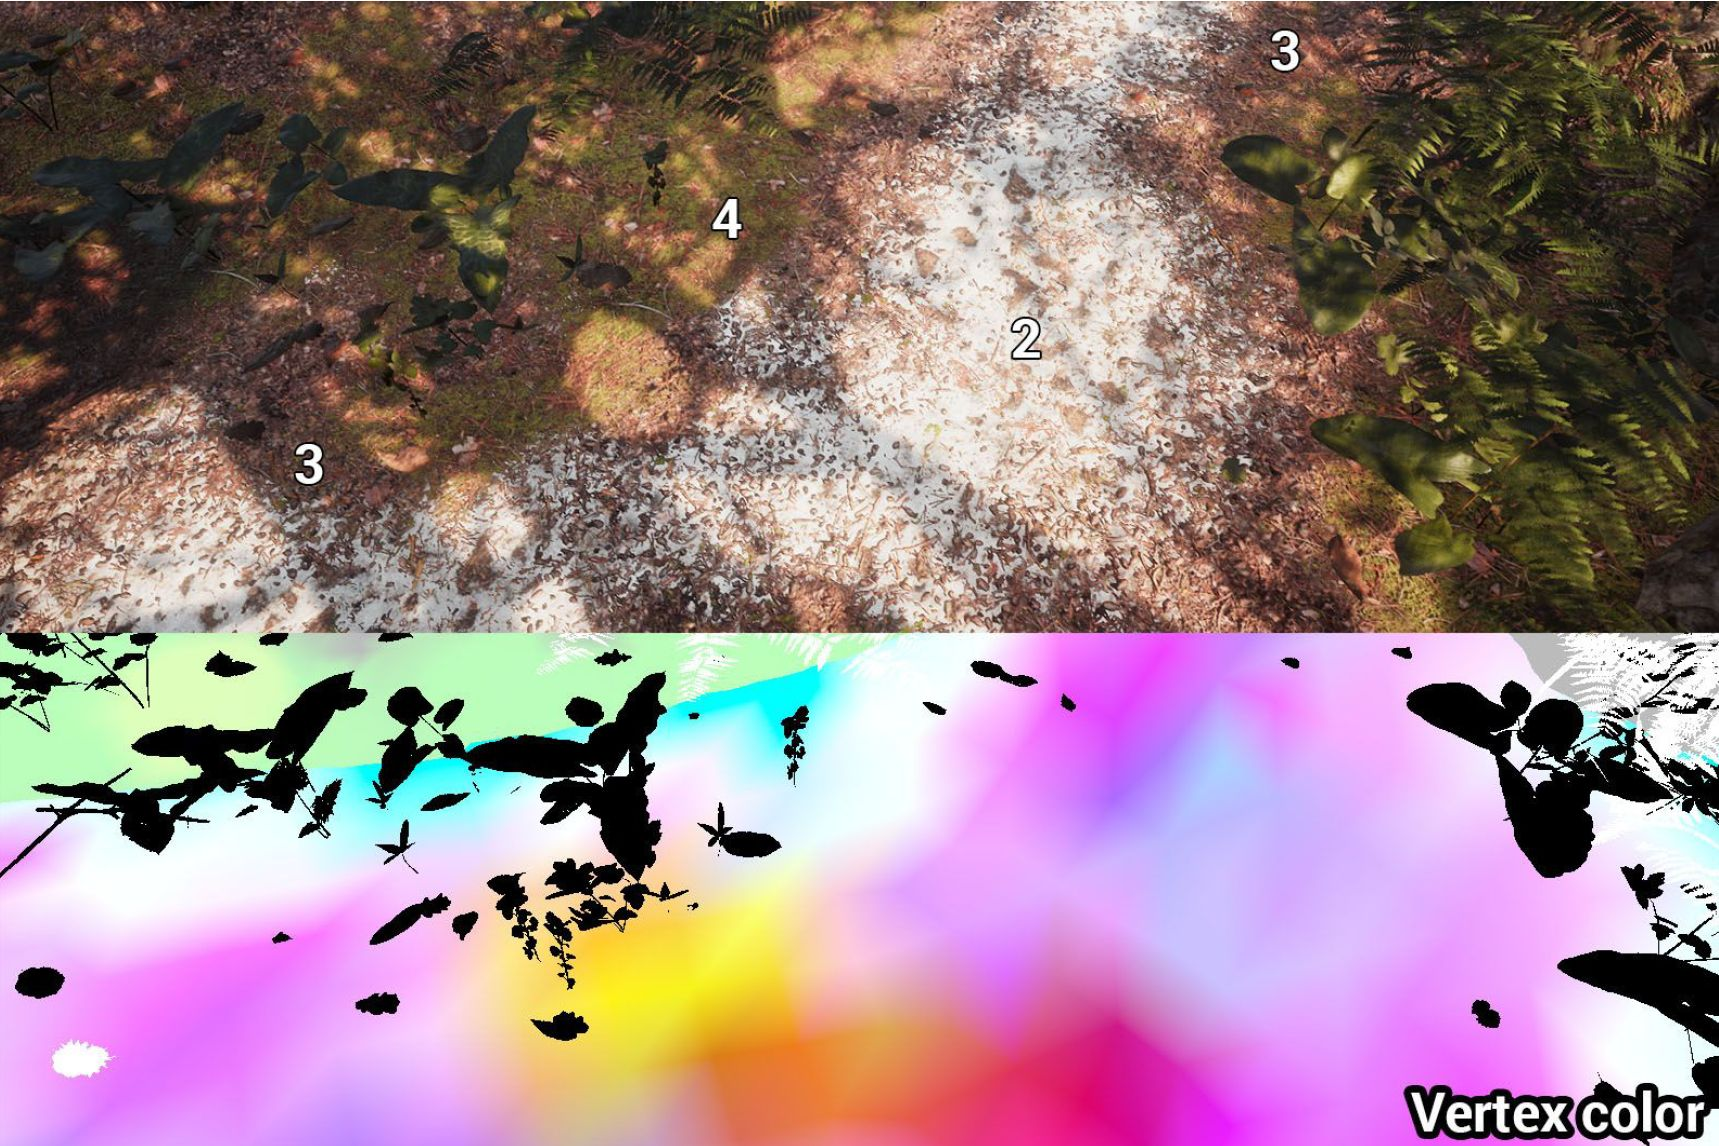
\includegraphics[width=.475\textwidth]{images/07cha_25_layeredLitUnity_vertex03.jpg} 
		\\
		(b) & (c) 
	\end{tabular}
	
	\caption{Using vertex paint to influence the base material blending and create surface variety. Image source: \cite[p.\,31--32]{unity2017photogrammetryLayered}.}
	\label{fig:vertexColor}
\end{figure}

%%%%%%%%%%%%%%%%%%%%%%%%%EXTERNAL INPUTS OBJECT DATA%%%%%%%%%%%%%%%%%%%%%%%%%%%%%%%%%%%%%%%

\subsection{\patCatObjectData}\label{\patCatObjectData}

While inputs connected to the mesh data are independent from other objects and their location within the 3D scene, object specific inputs are influenced by them. Object related values like hierarchy, position, rotation, scale are object data inputs. 

\subsubsection{\patObjectDataVectors}\label{\patObjectDataVectors}
\begin{description}
	\item[\patIntent:]% 
	Use different vectors to manipulate the material based on location, scale and rotation. 
	%\item[\patAlsoKnownAs:]% 
	\item[\patMotivation:]% 
	These vectors can be used to manipulate the other material parameter inputs. They could be used to manipulate an object depending on its position, rotation or scale. One possible use case for this can be to add a pseudo random variation---like random tint---to objects, depending on there position in space. The possible use cases are infinite as these vectors can be used to manipulate any parameter from color, saturation, roughness to UV coordinates. This kind of use does not work with moving object because the values update dynamically at runtime. Changing the translation, rotation or scale would therefore directly affects the material appearance at runtime.
	\item[\patApplicability:]\hfill 
	\begin{itemize}\mynobreakpar
		\item The objects have different location, scale or rotation values to drive procedural functions within the shader. 
		\item The specified vector does not change (e.g., If the random color is linked to the object position, the object should not be movable).
		\item Objects cannot be merged because it would combine them into one single object, with shared location, rotation and scale vectors. Therefore, all variety would be lost. 
	\end{itemize}
	\item[\patImplementation:]% 
	\emph{Unreal Engine 4} allows to access the object position, orientation and bounding box data really easily within the material editor.
	%\item[\patExamples:]% 
	\item[\patConsequences:]\hfill 
		\begin{description}
			\item[\visual:]\hfill
			\begin{itemize}\mynobreakpar
				\item This method provides an easy, fast and cheap way to create pseudo random values. 
			\end{itemize}
			\item[\performance:]\hfill
			\begin{itemize}\mynobreakpar
				\item It is cost efficient as it represents a simple vector based input in the shader graph. 
			\end{itemize}
			\item[\pipeline:]\hfill
			\begin{itemize}\mynobreakpar
				\item It is easy to implement. 
				\item Using different object vectors to drive pseudo random values is unstable. For instance, combining the object does destroy this effect.
				\item Changing the position of an object does change its look, which might be an unintended side effect. 
			\end{itemize}
		\end{description}
	\item[\patRelations:]% 
	This pattern can easily be implemented in an \emph{\patImplementationCustomShader} (section \ref{\patImplementationCustomShader})
\end{description}


\section{Summary}

The patterns presented in this chapter cover huge areas connected to pattern layering. They provide different possibilities on how to incorporate pattern layering into your pipeline and how to structure and organize the single components. Besides, they illustrate what alternatives exist to pattern layering. This chapter provided different solutions on how to implement the individual components: material container, masking container and blending module and how to utilize different input types. The potential for further work in this field will be presented in the next chapter.


